% Options for packages loaded elsewhere
\PassOptionsToPackage{unicode}{hyperref}
\PassOptionsToPackage{hyphens}{url}
%
\documentclass[
  12pt,
  a4paper,
  oneside]{book}
\usepackage{lmodern}
\usepackage{setspace}
\usepackage{amssymb,amsmath}
\usepackage{ifxetex,ifluatex}
\ifnum 0\ifxetex 1\fi\ifluatex 1\fi=0 % if pdftex
  \usepackage[T1]{fontenc}
  \usepackage[utf8]{inputenc}
  \usepackage{textcomp} % provide euro and other symbols
\else % if luatex or xetex
  \usepackage{unicode-math}
  \defaultfontfeatures{Scale=MatchLowercase}
  \defaultfontfeatures[\rmfamily]{Ligatures=TeX,Scale=1}
\fi
% Use upquote if available, for straight quotes in verbatim environments
\IfFileExists{upquote.sty}{\usepackage{upquote}}{}
\IfFileExists{microtype.sty}{% use microtype if available
  \usepackage[]{microtype}
  \UseMicrotypeSet[protrusion]{basicmath} % disable protrusion for tt fonts
}{}
\makeatletter
\@ifundefined{KOMAClassName}{% if non-KOMA class
  \IfFileExists{parskip.sty}{%
    \usepackage{parskip}
  }{% else
    \setlength{\parindent}{0pt}
    \setlength{\parskip}{6pt plus 2pt minus 1pt}}
}{% if KOMA class
  \KOMAoptions{parskip=half}}
\makeatother
\usepackage{xcolor}
\IfFileExists{xurl.sty}{\usepackage{xurl}}{} % add URL line breaks if available
\IfFileExists{bookmark.sty}{\usepackage{bookmark}}{\usepackage{hyperref}}
\hypersetup{
  pdftitle={RESTful Scraping API for Real Estate data, a Spatial Bayesian modeling perspective with INLA},
  pdfauthor={Niccolò Salvini},
  hidelinks,
  pdfcreator={LaTeX via pandoc}}
\urlstyle{same} % disable monospaced font for URLs
\usepackage[left=4cm, right=3cm, top=3cm, bottom=3cm]{geometry}
\usepackage{listings}
\newcommand{\passthrough}[1]{#1}
\lstset{defaultdialect=[5.3]Lua}
\lstset{defaultdialect=[x86masm]Assembler}
\usepackage{longtable,booktabs}
% Correct order of tables after \paragraph or \subparagraph
\usepackage{etoolbox}
\makeatletter
\patchcmd\longtable{\par}{\if@noskipsec\mbox{}\fi\par}{}{}
\makeatother
% Allow footnotes in longtable head/foot
\IfFileExists{footnotehyper.sty}{\usepackage{footnotehyper}}{\usepackage{footnote}}
\makesavenoteenv{longtable}
\usepackage{graphicx,grffile}
\makeatletter
\def\maxwidth{\ifdim\Gin@nat@width>\linewidth\linewidth\else\Gin@nat@width\fi}
\def\maxheight{\ifdim\Gin@nat@height>\textheight\textheight\else\Gin@nat@height\fi}
\makeatother
% Scale images if necessary, so that they will not overflow the page
% margins by default, and it is still possible to overwrite the defaults
% using explicit options in \includegraphics[width, height, ...]{}
\setkeys{Gin}{width=\maxwidth,height=\maxheight,keepaspectratio}
% Set default figure placement to htbp
\makeatletter
\def\fps@figure{htbp}
\makeatother
% Make links footnotes instead of hotlinks:
\DeclareRobustCommand{\href}[2]{#2\footnote{\url{#1}}}
\setlength{\emergencystretch}{3em} % prevent overfull lines
\providecommand{\tightlist}{%
  \setlength{\itemsep}{0pt}\setlength{\parskip}{0pt}}
\setcounter{secnumdepth}{5}
% \usepackage{color}
% \usepackage{fancyvrb}
% \newcommand{\VerbBar}{|}
% \newcommand{\VERB}{\Verb[commandchars=\\\{\}]}
% % Add ',fontsize=\small' for more characters per line
% \DefineVerbatimEnvironment{Highlighting}{Verbatim}{commandchars=\\\{\}}
% \usepackage{framed}
% \definecolor{shadecolor}{RGB}{248,248,248}
% \newenvironment{Shaded}{\begin{snugshade}}{\end{snugshade}}
\usepackage{booktabs}
\usepackage{pdfpages}
\usepackage{amsthm}
\usepackage{tabu}
\usepackage{booktabs}
\usepackage{longtable}
\usepackage{array}
\usepackage{multirow}
\usepackage{wrapfig}
\usepackage{float}
\usepackage{colortbl}
\usepackage{pdflscape}
\usepackage{algorithm2e}
\usepackage{tabu}
\usepackage{threeparttable}
\usepackage{threeparttablex}
\usepackage[normalem]{ulem}
\usepackage{makecell}
\usepackage{xcolor}
\lstset{
  breaklines=true
}
\makeatletter
\def\thm@space@setup{%
  \thm@preskip=8pt plus 2pt minus 4pt
  \thm@postskip=\thm@preskip
}
\makeatother
\let\oldmaketitle\maketitle
\AtBeginDocument{\let\maketitle\relax}
\usepackage{booktabs}
\usepackage{longtable}
\usepackage{array}
\usepackage{multirow}
\usepackage{wrapfig}
\usepackage{float}
\usepackage{colortbl}
\usepackage{pdflscape}
\usepackage{tabu}
\usepackage{threeparttable}
\usepackage{threeparttablex}
\usepackage[normalem]{ulem}
\usepackage{makecell}
\usepackage{xcolor}
\usepackage[]{natbib}
\bibliographystyle{apalike}

\title{RESTful Scraping API for Real Estate data, a Spatial Bayesian modeling perspective with INLA}
\author{\href{https://niccolosalvini.netlify.app/}{Niccolò Salvini}}
\date{Lastest build: 13 gennaio, 2021}

\usepackage{amsthm}
\newtheorem{theorem}{Theorem}[chapter]
\newtheorem{lemma}{Lemma}[chapter]
\newtheorem{corollary}{Corollary}[chapter]
\newtheorem{proposition}{Proposition}[chapter]
\newtheorem{conjecture}{Conjecture}[chapter]
\theoremstyle{definition}
\newtheorem{definition}{Definition}[chapter]
\theoremstyle{definition}
\newtheorem{example}{Example}[chapter]
\theoremstyle{definition}
\newtheorem{exercise}{Exercise}[chapter]
\theoremstyle{remark}
\newtheorem*{remark}{Remark}
\newtheorem*{solution}{Solution}
\begin{document}
\maketitle


\includepdf[pages={1}, scale=1]{cover.pdf}
\newpage

\let\maketitle\oldmaketitle
\maketitle

{
\setcounter{tocdepth}{2}
\tableofcontents
}
\listoftables
\listoffigures
\setstretch{1.5}
\hypertarget{intro}{%
\chapter{Introduction}\label{intro}}

Trento:

\begin{itemize}
\tightlist
\item
  Argomento
\item
  Problema
\item
  Obiettivi
\item
  Metodo
\item
  Struttura della tesi
\end{itemize}

Main themes:

\begin{itemize}
\tightlist
\item
  Research Question
\item
  Milan Real Estate Controversies in relation to research question
\item
  why the API (perchè mi mancano i dati e perchè è il futuro)
\item
  Open Data discussion personal hope of data sharing and benefits from oper source
\item
  Why a Bayesian approach
\item
  Why INLA
\end{itemize}

According to Google research devoted to the analysis of USA real estate
buyers' habits (National Association of Realtors, Google 2012), out of 10 \%
homebuyers use the Internet as one of the primary research tools, and 52 \% of
customers start their search using the Internet. According to the information
presented by Google, the number of real estate searches grows up yearly by 22 \%.
The main reason for customers is to find information which can reduce purchasing
related risks (Peterson \& Merino, 2003).
In Latvia, 79.7 \% of the population now goes online regularly (Latvijas
Interneta Asociācija, 2015). Latvian Internet users have the same habits as the
Internet users of the USA or developed Western countries. 7 out of 10 Internet
users (70 \%) look for information on web pages (CSP, 2015). Real estate buyers
read general information about a real estate object and compare prices of various
real estate objects

As a general discussion technologies implied can be thought as the distance between a service running locally on a laptop and something that it can actually be put into production, shared among company stakeholders, solving business related problems. When such technologies are applied data scientist and interlocutors gradually close the gap. Insights are better communicated, data is up-to-date and automation can save time. Nonetheless when the infrastructure is structured with vision then integrating or substituting existing technologies is not trivial. Anyway technologies can not be always embedded because they might be exclusively designed to work only on certain back ends, therefore some choices are not into discussion. With foresight RStudio by setting future-oriented guidelines has spent a lot of effort giving its users an easy, integrated and interconnected environment. By that it is meant that the RStudio community has tried to either integrate or open the possibility to a number of technologies that fill the blanks in their weaker parts. On top of many, an entire package has been dedicated to democratize REST APIs (Plumber \citep{plumber}). As a further example developers in RStudio have created an entire new paradigm i.e.~Shiny \citep{shiny}, a popular web app development package, that enforces the developer to have front-end and back-end technologies tied up in the same IDE. They also added performance monitoring and optimization packages that are fitted into shiny such as shinytest {[}metti tag{]} and shinyloadtest {[}metti tag{]} to simulate sessions and verify network traffic congestion.

\hypertarget{scraping}{%
\chapter{Web Scraping}\label{scraping}}

The following chapter covers a modern technique and up-to-date libraries for web scraping in R and related challenges with a focus on the immobiliare.it case. The easiest way of collecting information from websites involves inspecting and manipulating URLs. While browsing web pages urls under the hood compose themselves in the navigation bar according to a certain encoded semantic, specifying domain, url paths and url parameters. As a matter of fact websites can be regarded as a complex system of nested folders where urls are the relative file path to access to the content desired. That implies if a function can mimic the url semantic by providing decoded, human-readable arguments, then any content in the website can be filtered and later accessed.
Once urls are reproduced and stored into a variable, scraping function are called on these set of address.
The major time improvement with respect to classical crawlers comes from retrieving a set of urls instead of gathering the entire website sitemap and then searching through keywords.
This is made exploiting a scraping workflow library, namely \passthrough{\lstinline!rvest!} \citet{rvest}, which takes inspiration from the scraping gold standard Python library Beautiful Soup \citet{Beautifulsoup}. A search algorithm strategy, calibrated on the specific scraping context, is nested inside scraping functions whose skeleton is reproduced for all the information demanded. The search strategy exploits different CSS queries that point to different data location within the web page, with the aim to be sure to carry out a comprehensive exploration and to deliver data where available. Functions are then wrapped up around a ``main'' function that simplifies portability and enables parallelization. Both of the search logic flows are fronted presenting their pseudocode.
HTTP protocol communication and related main concepts are introduced with the aim to familiarize with internet communication layers focusing on traffic from web server to web clients and viceversa and principal actors involved.
By doing that some opinionated but highly diffused scraping best practices are incorporated into scraping taking inspiration by a further R library \passthrough{\lstinline!Polite!} \citet{polite}. Revised best practices try to balance scraping efficiency and \emph{web etiquette}. As a result optimization happens both from the \emph{web server} side; this is tackled by kindly asking for permission and sending delayed server requests rate based on Robotstxt file requirements. As well as from the \emph{web client} by preventing scraping discontinuity caused by server blocks thanks to \emph{User Agent} (HTTP request headers) pool \emph{rotation} and \emph{fail dealers}.
\emph{Parallel} computing is carried out due to data obsolescence, since the market on which scraping functions are called is vivid and responsive. At first concepts and are introduced and then main centered on the specific R parallel ecosystem. Then a run time scraping benchmark is presented for two different modern parallel back end options \passthrough{\lstinline!future!} \citet{future} and \passthrough{\lstinline!doParallel!} \citet{doParallel}, along with two parallel looping paradigma, \passthrough{\lstinline!furrr!} \citet{furrr} and \passthrough{\lstinline!foreach!} \citet{foreach}. Both of the two combinations have showed similar results, nevertheless the former offers a more \{Tidiverse\} coherence and a more comfortable debugging experience.
Furthermore an overview of the still unlocked challenges is provided on the open source project and possible improvements, with the sincere hope that the effort put might be extended or integrated. In the end a heuristic overview on the main legal aspect is offered bringing also an orientation inspired by a ``fair balance'' trade off between web scraping practices and the most common claims. Then a court case study about a well known scraping litigation is brought demonstrating how law is not solid in this area and how scrapign market should find its own equilibrium.

\hypertarget{reverse}{%
\section{A Gentle Introduction on Web Scraping}\label{reverse}}

\begin{definition}[Scraping]
\protect\hypertarget{def:scraping}{}{\label{def:scraping} \iffalse (Scraping) \fi{} }Web Scraping is a technique aimed at extracting unstructured data from static or dynamic internet web pages and collecting it in a structured way.
Automated data collection, web extraction, web crawling, or web data mining are often used as synonyms to web scraping.
\end{definition}

The World Wide Web (WWW or just the web") data accessible today is calculated in zettabytes \citep{ciscooutlook} (\(1\) zettabyte = \(10^{21}\) bytes). This huge volume of data provides a wealth of resources for researchers and practitioners to obtain new insights in real time regarding individuals, organizations, or even macro-level socio-technical phenomena \citep{krotovtennyson}. Unsurprisingly, researchers of Information Systems are increasingly turning to the internet for data that can address their research questions \citeyearpar{krotovtennyson}. Taking advantage of the immense web data also requires a programmatic approach and a strong foundation in different web technologies.
Besides the large amount of web access and data to be analyzed, there are three rather common problems related to big web data: variety, velocity, and veracity \citep{LegalityEthicsWS}, each of which exposes a singular aspect of scraping and constitutes some of the challenges fronted in later chapters.
\emph{Variety} mainly accounts the most commonly used mark-up languages on the web used for content creation and organization such as such as HTML \citep{html_2020}, CSS \citep{css_2020}, XML \citep{wiki:XML} and JSON \citep{wiki:JSON}. Sometimes Javascript \citep{wiki:Javascript} components are also embedded into websites. In this cases dedicated parsers are required which would add a further stumbling block. Starting from these points scraping requires at least to know the ropes of these technologies which are also assumed in this analysis. Indeed later a section will be partially dedicated to familiarize with the inner internet mechanism taht manages the exhanges of information, such as HTTP protocols.
\emph{Velocity}: web data are in continuous flow status: it is created in real time, modified and changed continuously. This massively impacts the analysis that relies on those data which, as times passes, becomes obsolete. However it also suggests the speed and pace at which data should be collected. From one hand data should be gathered as quicker as possible so that analysis or softwares are up-to-date, section \ref{parallelscraping}. From the other this should happen in any case by constraining speed to common shared scraping best practices, which require occasional rests in requesting information. The latter issue is faced later in section \ref{best-practices}.
\emph{Veracity}: Internet data quality and usability are still surrounded by confusion. A researcher can never entirely be sure if the data he wants are available on the internet and if the data are sufficiently accurate to be used in analysis. While for the former point data can be, from a theoretical perspective, accurately selected it can not be by any means predicted to exist. This is a crucial aspects of scraping, it should take care of dealing with the possibility to fail, in other words to be lost. The latter point that points to data quality is also crucial and it is assessed by a thoughtful market analysis that mostly assures the importance of immobiliare.it as a top player in italian real estate. As a consequence data coming from reliable source is also assumed to be reliable.
Furthermore web scraping can be mainly applied in two common forms as in \citep{wsstatistics}: the first is browser scraping, where extractions takes place through HTML/XML parser with regular expression matching from the website's source code. The second uses programming interfaces for applications, usually referred to APIs. The main goal of this chapter is to combine the two by shaping a HTML parser and make the code portable into an RESTful API whose software structure is found at \ref{infrastructure}.
Regardless of how difficult it is the process of scraping, the circle introduced in \citet{automateddatacollection} and here revised with respect to the end goal, is almost always the same. Most scraping activities include the following sequence of tasks:

\begin{itemize}
\tightlist
\item
  Identification of data
\item
  Algorithm search Strategy
\item
  Data collection
\item
  Data preprocess
\item
  Data conversion
\item
  Debugging and maintenance
\item
  Portability
\end{itemize}

Scraping essentially is a clever combination and iteration of the previous tasks which should be heavily shaped on the target website or websites.

\hypertarget{anatomy-of-a-url-and-reverse-engineering}{%
\section{Anatomy of a url and reverse engineering}\label{anatomy-of-a-url-and-reverse-engineering}}

Uniform Resource Locators (URLs) \citep{wiki:url}, also known as web addresses, determine the location of websites and other web contents and mechanism to retrieve it.
Each URL begins with a scheme, purple in figure \ref{fig:urlanatomy}, specifying the protocol used to communicate client-application-server contact i.e.~HTTPS. Other schemes, such as ftp (File transmission protocol) or mailto for email addresses correspond to SMTP (Simple Mail Transfer Protocol) standards.

\begin{figure}
\centering
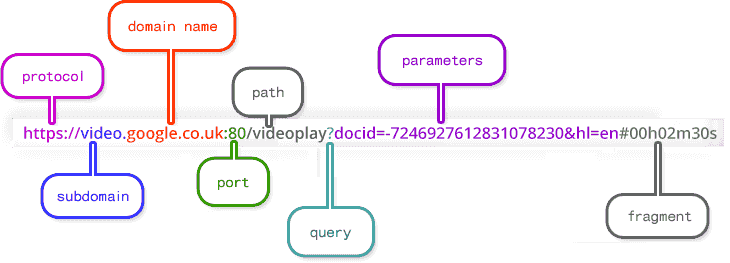
\includegraphics{images/complex_url.png}
\caption{\label{fig:urlanatomy}General url Anatomy, \citet{Anatomyo72} source}
\end{figure}

The \emph{domain name} in red in figure \ref{fig:urlanatomy}, with a specific ID, indicates the server name where the interest resource is stored. The domain name is sometimes accompanied with the \emph{port} whose main role is to point to the open door where data transportation happens. Default port for Transmission Control Protocol ( \emph{TCP} ) is 80. In the following chapter ports will play a crucial role since a compose file wiill instruct containers (\ref{docker}) to open and route communication through these channels and then converge the whole traffic into a secured one \ref{nginx}.
Typically domain name are designed to be human friendly, indeed any domain name has its own proprietary IP and public IP (IPv4 and IPv6) address which is a complex number, e.g.~local machine IP is 95.235.246.91. Here intervenes \emph{DNS} whose function is to redirect domain name to IP and vice versa. The path specifies where the requested resource is located on the server and typically refers to a file or directory. Moving towards folders requires name path locations separated by slashes. In certain scenarios, URLs provide additional \emph{path} information that allows the server to correctly process the request. The URL of a dynamic page (those of who are generated from a data base or user-generated web content) sometimes shows a \emph{query} with one or more parameters followed by a question mark. \emph{Parameters} follow a ``field=value'' scheme each of which is separated by a ``\&'' character for every different parameter field, 6th character from the end in figure \ref{fig:urlanatomy} parameter space. Each further parameter field added is appended at the end of the url string enabling complex and specific search queries.
\emph{Fragments} are an internal page reference often referred to as an anchor. They are typically at the end of a URL, starting with a hash (\#) and pointing to specific part of a HTML document. Note that this is a full browser client-side operation and fragments are used to display only certain parts of already rendered website.
The easiest way of collecting information from websites often involves inspecting and manipulating URLs which refer to the content requested. Therefore urls are the starting point for any scraper and they are also the only functional argument to be feeding to. Url parameters indeed help to route web clients to the requested information and this is done \emph{under the hood} and unconsciously while the user is randomly browsing the web page.
Let us assume to express the necessity to scrape only certain information from a generic website.
Then if this data to be scraped can be circumscribed by properly setting url parameters, under those circumstances it is also demanded a way to consciously compose these urls. In other words a function (or a sevice) needs to mould urls by mimicking their mutations operated by browser while the user is navigating. As a matter of fact as filters (i.e.~parameters) are applied to the initial search page for immobiliare.it then parameters populate the navigation bar. For each of the filters specified a new parameter field and its own selected value are appended to the url string according to the website specific \emph{semantic}. Each website has its own sematic.
As an example are applied directly to the domain name \passthrough{\lstinline!https://www.immobiliare.it/!} the following filters (this is completely done in the dedicated panel):

\begin{itemize}
\tightlist
\item
  rental market (the alternative is selling)
\item
  city is Milan
\item
  bathrooms must be 2
\item
  constrained zones search on ``Cenisio'' and ``Fiera''
\end{itemize}

The resulting url is:

\begin{figure}
\centering
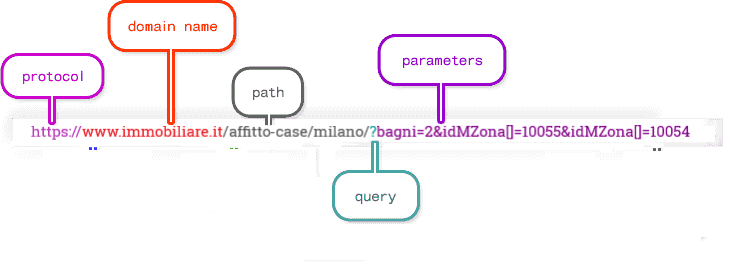
\includegraphics{images/immobiliare_url.png}
\caption{\label{fig:urlanatomy}immobiliare url composed according to some filters, author's source}
\end{figure}

At first glance immobiliare.it does not enact a \emph{clean url} \citep{wiki:cleanurl} structure, which ultimately would simplify a lot the reverse sematic process.
In truth parameters follows a chaotic semantic. While the filter city=``milano'' is located in the url path the remaining are transferred to the url parameters. For some of them the logical trace back from the parameter field-value to their exact meaning is neat, i.e.~bagni=2 and can be said clean. Unfortunately for the others the sematinc is not obvious and requires a further reverse layer to deal with.
In addition to this fact the url in figure \ref{fig:urlanatomy} readdress to the very first page of the search meeting the filter requirements, which groups the first 25 rental advertisements. The following set of 25 items can be reached by relocating the url address to:
\passthrough{\lstinline!https://www.immobiliare.it/affitto-case/milano/?bagni=2\&idMZona[]=10055\&idMZona[]=10054\&pag=2!}. The alteration regards the last part of the url and constitutes a further url parameter field to look for. Note that the first url does not contain ``\&pag=1''. For each page browsed by the user the resulting url happen to be the same plus the prefix ``\&pag='' glued with the correspondent \(n\) page number (from now on referred as \emph{pagination}). This is carried on until pagination reaches either a stopping criteria argument or the last browsable web page (pagination sets as default option 10 pages, which returns a total of 250 rental advertisement).
Therefore for each reversed semantic url are obtainable 25 different links, see figure \ref{fig:nestedstructure} that is where actually are disclosed relevant data and the object of scraping. Links belonging to the 25 items set share the same anatomy: \passthrough{\lstinline!https://www.immobiliare.it/annunci/84172630/!} where the last \emph{path} is associated to a unique
ID, characteristic of the rental property. Unfortunately there is not any available solution to retrieve all the existing ID, therefore links needs to collected directly from ``main'' url in figure \ref{fig:urlanatomy} as an obvious choice.

\begin{figure}
\centering
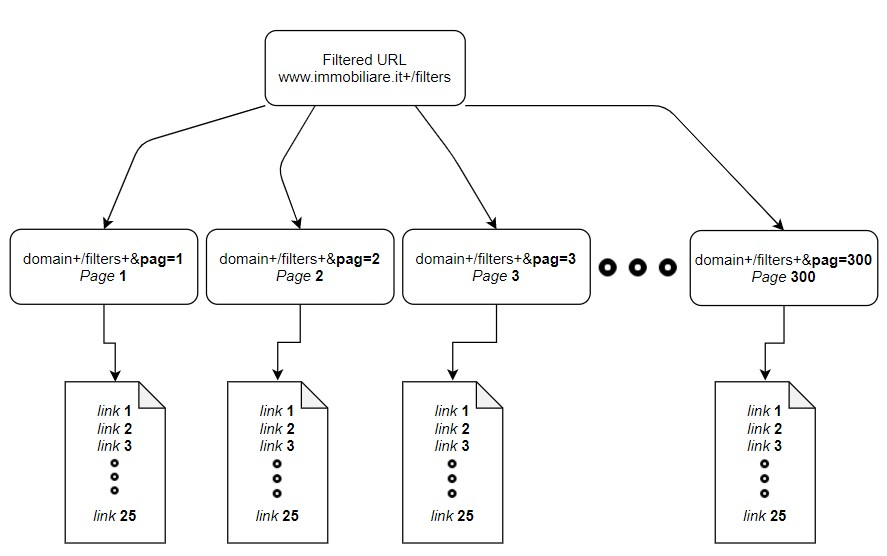
\includegraphics{images/website_tree1.jpg}
\caption{\label{fig:nestedstructure}immobiliare.it website structure, author's source}
\end{figure}

Therefore 4 steps are required to \emph{reverse engineer} the url \citeyearpar{automateddatacollection} and to ultimately make the links access available:

\begin{enumerate}
\def\labelenumi{\arabic{enumi}.}
\tightlist
\item
  Determine how the URL syntactic works for each parameter field
\item
  Build the url based on the reverse engineered sematic:

  \begin{enumerate}
  \def\labelenumii{\alph{enumii}.}
  \tightlist
  \item
    those ones who need an ID parameter value
  \item
    clean ones who need to only explicit the parameter value
  \end{enumerate}
\item
  Pagination is applied to the url until stopping criteria are met
\item
  Obtain the links for each urls previously generated
\end{enumerate}

Once identified the inner composition mechanism by an insistent trial and error then the url restoration could starts. Parameter values for those that requires an ID in figure \ref{fig:urlanatomy} are encoded is a way that each number is associated to its respective zone ID e.g.~as in figure \ref{fig:urlanatomy} ``Fiera'' to 10055 or ``Cenisio'' to 10054. Therefore a decoding function should map the parameter value number back to the correspondent human understandable name e.g from 10055 to ``Fiera'' or 10054 to ``Cenisio'', the exactly opposite logical operation. The decoding function exploits a JSON database file that matches for each ID its respective zone name exploiting suitable JSON properties. The JSON file is previously compounded by generating a number of random url queries and subsequently assigning the query names to their respective ID. As soon as the JSON file is populated the function can take advantage of that database and compose freely urls at need. Pagination generates a set of urls based on the number of pages requested. In the end for each urls belonging to the set of urls, links are collected by a dedicated function and stored into a vector. Furthermore if the user necessitate to directly supply a precomposed url the algorithm overrides the previous object and applies pagination on the provided url. The pseudocode in figure \ref{fig:pseudocode3} paints the logic behid the reverse egineering process.

\begin{figure}
\centering
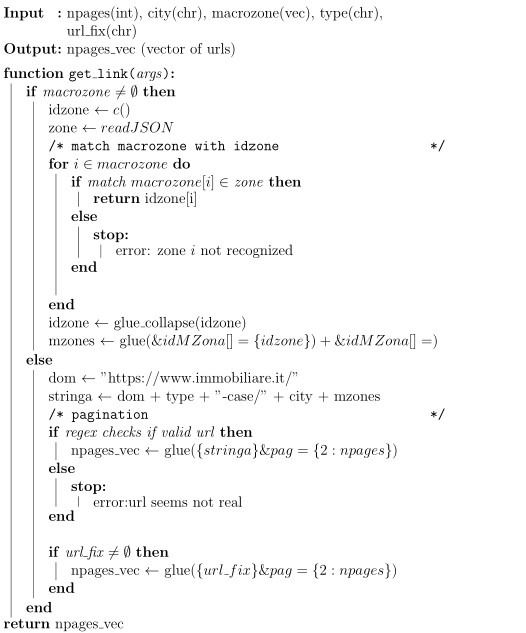
\includegraphics[width=0.7\textwidth,height=\textheight]{images/pseudocode_latex/pseudocode_get_link.jpg}
\caption{\label{fig:pseudocode3}pseudo code algorithm to reverse engineer url, author's source}
\end{figure}

\hypertarget{scraping-with-rvest}{%
\subsection{\texorpdfstring{Scraping with \texttt{rvest}}{Scraping with rvest}}\label{scraping-with-rvest}}

Reverse engineered urls are then feeded to the scraper which arranges the process of scraping according to the flow chart imposed by \passthrough{\lstinline!rvest!} in figure \ref{fig:rvestflowchart}. The sequential path followed is highlighted by the light blue wavy line and offers one solution among all the alternative ways to get to the final content. The left part with respect to the central dashed line of figure \ref{fig:rvestflowchart} takes care of setting up the session and parsing the response. As a consequence at first scraping in consistent way requires to open a session class object with \passthrough{\lstinline!html\_session!}. Session arguments demands both the target url, as built in \ref{fig:pseudocode3} and the request headers that the user may need to send to the web server. Data attached to the web server request will be further explored later in section\ref{spoofing}, tough they are mainly 4: User Agents, emails references, additional info and proxy servers. The session class objects contains a number of useful data regarding either the user log info and the target website such as: the url, the response, cookies, session times etc. Once the connection is established (response 200), functions that come after the opening rely on the object and its response. In other words while the session is happening the user will be authorized with the already provided headers data. As a result jumps from a link to the following within the same session are registered by in the object. Most importantly sessions contain the xml/html content response of the webpage, that is where data needs to be accessed.

\begin{figure}
\centering
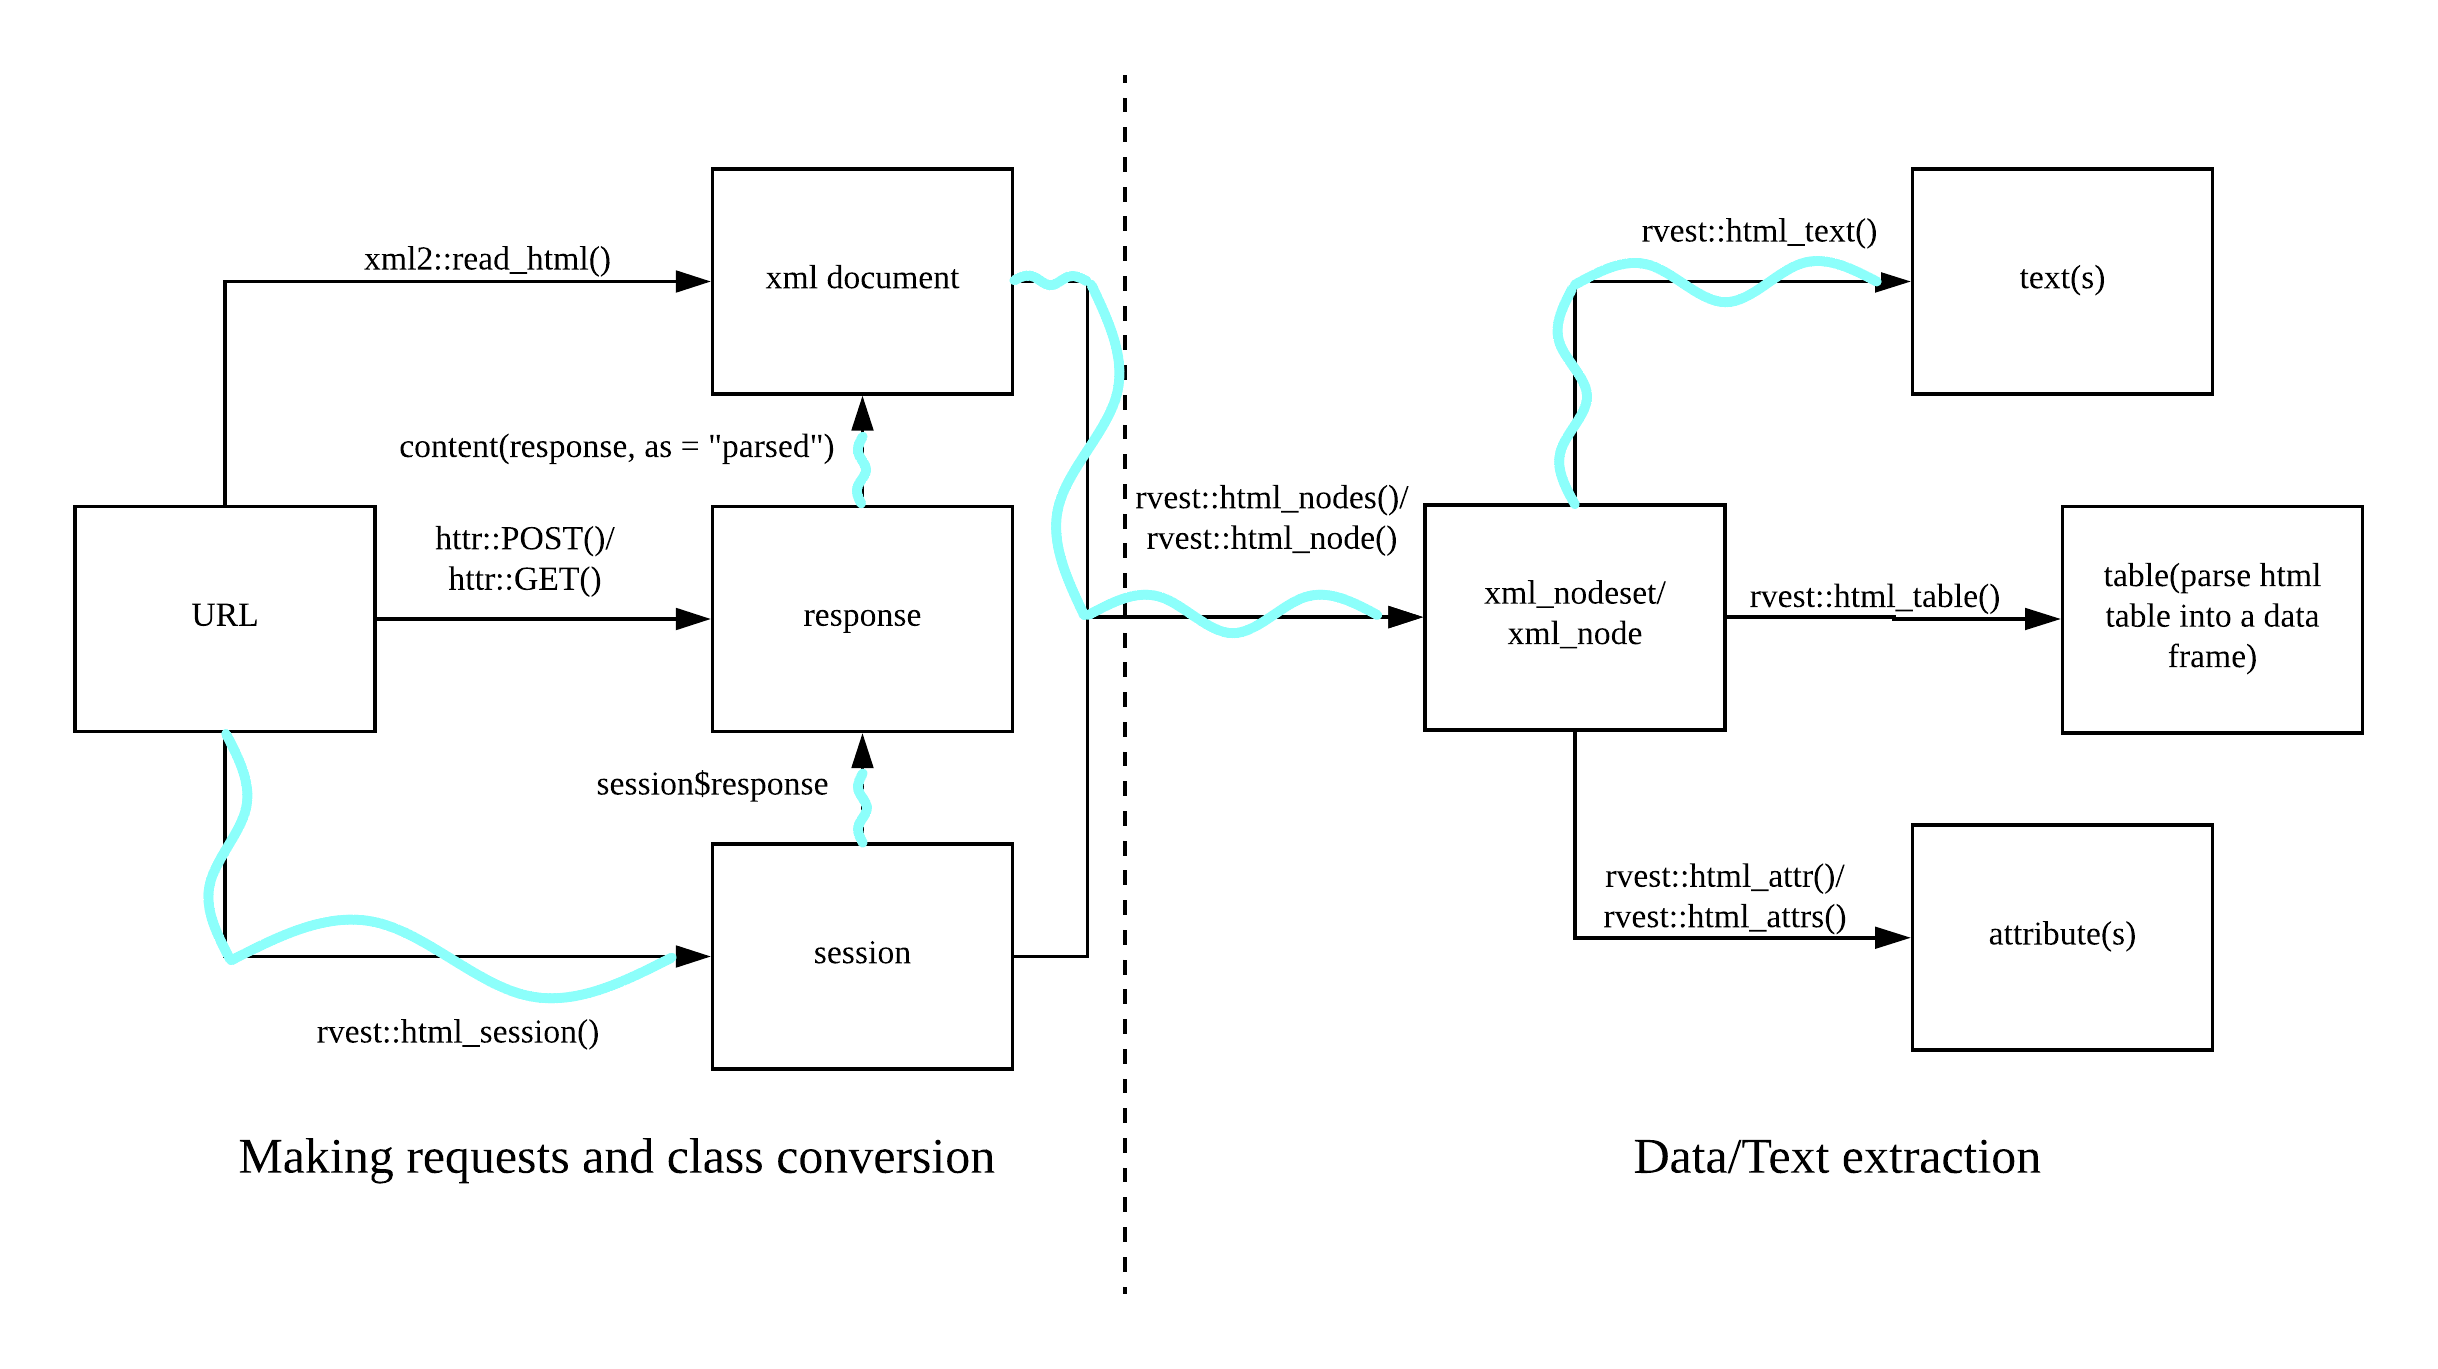
\includegraphics{images/workflow.png}
\caption{\label{fig:rvestflowchart}rvest general flow chart, author's source}
\end{figure}

Indeed at the right of dashed line in \ref{fig:rvestflowchart} are represented the last two steps configured into two \passthrough{\lstinline!rvest!}\citep{rvest} functions that locate the data within the HTML nodes and convert it into a human readble text, i.e.~from HTML/XML to text. The most of the times can be crafty to find the exact HTML node or nodes set that contains the data wanted, expecially when HTML trees are deep nested and dense. html\_node function provides and argument that grants to specify a simple CSS/XPATH selector which may group a set of HTML/XML nodes or a single node. Help comes from an open source library and browser extension technology named SelectorGadget. SelectorGadget \citep{Selectorgadget} which is a JavaScript bookmark that allows to interactively explore which CSS selector is needed to gather desired components from a webpage. Data can be repeated many times into webpages so the same information can be found at multiple CSS queries. This fact highlights one of the priciples embodied in the follwing section \ref{ProperScraping} accroding to which searching methods gravitates. Once the CSS query points address to the desired content then data finally needs to be converted into text. This is what explicitly achieve hmlt\_text.

\hypertarget{ProperScraping}{%
\section{Searching Technique for Scarping}\label{ProperScraping}}

The present algorithm in figure \ref{fig:pseudocode1} imposes a nested sequential search strategy and gravitates around the fact that data within the same webpage is repeated many times, so multiple CSS queries are avaialble for the same information. Furthermore since data is repeated has also less probability to be missed. CSS sequential searches are calibrated from the highest probability of appearance in that CSS selector location to the lowest so that most visited locations are also the the most likely to grab data.
A session object \passthrough{\lstinline!opensess!}, the one seen in \ref{fig:rvestflowchart}), is initialized sending urls built in \ref{fig:pseudocode3}. The object opensess constitutes a check point obj because it is reused more than once along the algorithm flow. The object contains session data as well as HTML/XML content. Immediately after another object \passthrough{\lstinline!price!} parses the sessions and points to a CSS query through a set of HTML nodes. The CSS location \passthrough{\lstinline!.im-mainFeatures\_\_title!} addresses a precise group of data which are found right below the main title. Expectations are that monthly price amount in that location is a single character vector string, containing price along with unnecessary non-UTF characters. Then the algorithm bumps into the first \passthrough{\lstinline!if!} statement. The logical condition checks whether the object \passthrough{\lstinline!price!} first CSS search went lost. If it does not the algorithm directly jumps to the end of the algorithm and returns a preprocessed single quantity. Indeed if it does it considers again the check point \passthrough{\lstinline!opensess!} and hits with a second css query \passthrough{\lstinline!.im-features\_\_value , .im-features\_\_title!}, pointing to a second data location. Note that the whole search is done within the same session (i.e.~reusing the same session object), so no more additional request headers \ref{spoofing} has to be sent). Since the second CSS query points to data sequentially stored into a list object, the newly initialized \passthrough{\lstinline!price2!} is a type list object containing various information. Then the algorithm flows through a second \passthrough{\lstinline!if!} statement that checks whether \passthrough{\lstinline!"prezzo"!} is matched in the list, if it does the algorithm returns the +1 position index element with respect to the ``prezzo'' position. This happens because data in the list are stored by couples sequentially (as a flattened list), e.g.~list(title, ``Appartamento Sempione'', energy class, ``G'', ``prezzo'', 1200/al mese). Then in the end a third CSS query is called and a further nested if statement checks the emptiness of the latest CSS query. \passthrough{\lstinline!price3!} points to a hidden JSON object within the HTML content. If even the last search is lost then the algorithm escapes in the else statement by setting \passthrough{\lstinline!NA\_Character\_!}, ending with any CSS query is able to find price data.
The search skeleton used for price scraping constitutes a standard reusable search method in the analysis for all the scraping functions. However for some of the information not all the CSS location points are available and the algorithm is forced to be rooted to only certain paths, e.g.~``condizionatore'' can not be found under main title and so on.

\begin{figure}
\centering
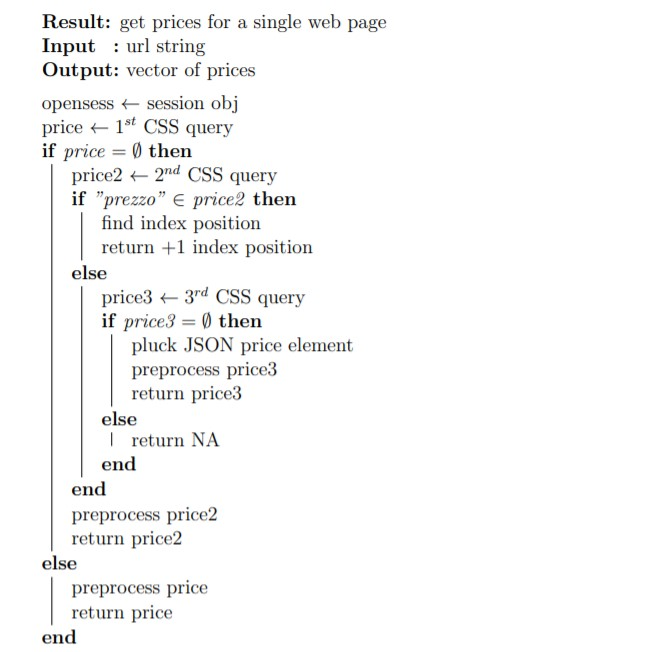
\includegraphics[width=0.7\textwidth,height=\textheight]{images/pseudocode_latex/pseudocode_price.jpg}
\caption{\label{fig:pseudocode1}pseudo code algorithm for price search, author's source}
\end{figure}

Once all the functions have been designed and optimized with respect to their scraping target they need to be grouped into a single ``main'' \emph{fastscrape} function, figure \ref{fig:pseudocode4}. This is accomplished into the API function endpoint addressed in section \ref{plumberapi}, which also applies some sanitization, next chapter section \ref{sanitize}, on users inputs and administers also some security API measures, as in \ref{DoS} outside the main function. Moreover as it will be clear in section \ref{parallelscraping} the parallel back end will be registered outside the scraping function for unexplained inner functioning reasons.

\begin{figure}
\centering
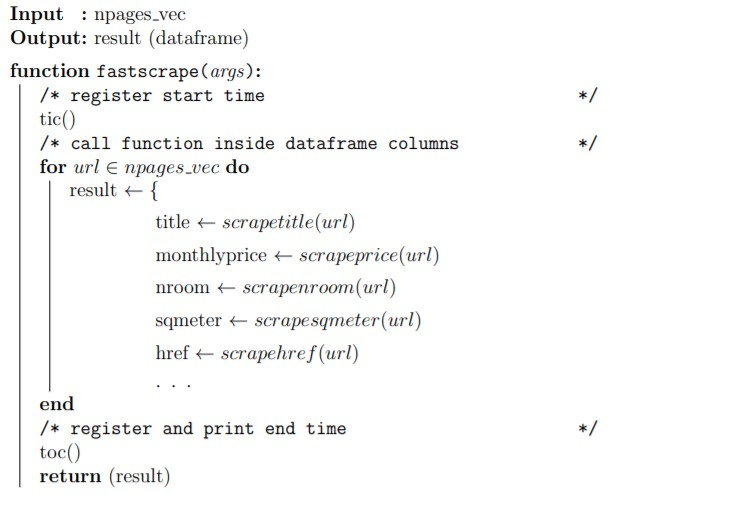
\includegraphics{images/pseudocode_latex/pseudocode_mainjpg.jpg}
\caption{\label{fig:pseudocode4}pseudo code algorithm structure for fatstscrape, author's source}
\end{figure}

\textbf{pseudo code}

\hypertarget{best-practices}{%
\section{Scraping Best Practices and Security provisions}\label{best-practices}}

Web scraping have to naturally interact multiple times with both the \emph{client} and \emph{server side} and as a result many precautions must be seriously taken into consideration. From the server side a scraper can forward as many requests as it could (in the form of sessions opened) which might cause a traffic bottleneck (DOS attack \citet{wiki:DOS}) impacting the overall server capacity. As a further side effect it can confuse the nature of traffic due to fake user agents \ref{spoofing} and proxy servers, consequently analytics reports might be driven off track.
Those are a small portion of the reasons why most of the servers have their dedicated Robots.txt files. Robots.txt \citet{meissner_2020} are a way to kindly ask webbots, spiders, crawlers to access or not access certain parts of a webpage. The de facto ``standard'' never made it beyond a \emph{informal} ``Network Working Group INTERNET DRAFT''. Nonetheless, the use of robots.txt files is widespread due to the vast number of web crawlers (e.g.~\href{https://en.wikipedia.org/robots.txt}{Wikipedia robot}, \href{https://www.google.com/robots.txt}{Google robot}). Bots from the own Google, Yahoo adhere to the rules defined in robots.txt files, although their \emph{interpretation} might differ.

Robots.txt files \citep{robotstxt} essentially are plain text and always found at the root of a website's domain. The syntax of the files follows a field-name value scheme with optional preceding user-agent. Blocks are separated by blank lines and the omission of a user-agent field (which directly corresponds to the HTTP user-agent field, cleared later in \ref{spoofing}) is seen as referring to all bots. The whole set of possible field names are pinpointed in \citet{google:robottxt}, some important are: user-agent, disallow, allow, crawl-delay, sitemap and host. Some common standard interpretations are:

\begin{itemize}
\tightlist
\item
  Finding no robots.txt file at the server (e.g.~HTTP status code 404) implies full permission.
\item
  Sub-domains should have their own robots.txt file, if not it is assumed full permission.
\item
  Redirects from subdomain www to the domain is considered no domain change - so whatever is found at the end of the redirect is considered to be the robots.txt file for the subdomain originally requested.
\end{itemize}

A comprehensive scraping library that observes a web etiquette is the \passthrough{\lstinline!polite!} \citep{polite} package. Polite combines the effects of \passthrough{\lstinline!robotstxt!}, \passthrough{\lstinline!ratelimitr!} \citeyearpar{ratelimitr} to limit sequential session requests together with the \passthrough{\lstinline!memoise!} \citep{memoise} for robotstxt response caching. Even though the solution meets the politeness requirements (from server and client side) ratelimitr is not designed to run in parallel as documented in the vignette \citep{ratelimitr}. This is a strong limitation as a result the library is not applied. However the 3 simple but effective web etiquette principles around, which is the package wrapped up, describe what are the guidelines for a ``polite'' session:

\begin{quote}
The three pillars of a polite session are seeking permission, taking slowly and never asking twice.

\hfill --- Dmytro Perepolkin, polite author
\end{quote}

The three pillars constituting the \emph{Ethical} web scraping manifesto \citep{densmore_2019} are considered as common shared \emph{best practices} that are aimed to self regularize scrapers. In any case these guidelines have to be intended as eventual practices and by no means as required by the law. However many scrapers themselves, as website administrators or analyst, have been fighting for many and almost certainly coming years with bots, spiders and derivatives. As a matter of fact intensive scraping might fake out real client navigation logs and confuse digital footprint, which results in induced distorted analytics. On the other hand if data is not given and APIs are not available, then scraping is sadly no more an option.
Therefore throughout this analysis the goal will be trying to find a well balanced trade-off between interests on the main actors involved.
Newly balanced (with respect to the author thought) guidelines would try to implement at first an obedient check on the validity of the path to be scraped through a cached function. Secondly it will try to limit request rates to a more feasible time delay, by keeping into the equation also the client time constraints. In addition it should also guarantee the continuity in time of scraping not only from the possibility to fail section \ref@(possibly)), but also from servers ``unfair'' denial (in section \ref{spoofing}).
With that said a custom function caches the results of robotstxt into a variable i.e.~\passthrough{\lstinline!polite\_permission!}. Then paths allowed are evaluated prior any scraping function execution. Results should either negate or affirm the contingency to scrape the following url address.

\begin{lstlisting}
## Memoised Function:
## [1] TRUE
\end{lstlisting}

\passthrough{\lstinline!polite\_permission!} is then reused to check, if any, the server suggestion on crawl relay. In this particular context no delays are kindly advised. As a default polite selection delay request rates are set equal to 2.5 seconds. Delayed are managed through the \passthrough{\lstinline!purrr!} stack. At first a \passthrough{\lstinline!rate!} object is initialized based on polite\_permission results, as a consequence a \passthrough{\lstinline!rate\_sleep!} delay is defined and iterated together with any request sent, as in \citet{rate_delay}.

\begin{lstlisting}[language=R]
get_delay = function(memoised_robot, domain) {
    
    message(glue("Refreshing robots.txt data for %s... {domain}"))
    temp = memoised_robot$crawl_delay
    
    if (length(temp) > 0 && !is.na(temp[1, ]$value)) {
        star = dplyr::filter(temp, useragent == "*")
        if (nrow(star) == 0) 
            star = temp[1, ]
        as.numeric(star$value[1])
    } else {
        2.5
    }
    
}
get_delay(rbtxt_memoised, domain = dom)
\end{lstlisting}

\begin{lstlisting}
## [1] 2.5
\end{lstlisting}

\hypertarget{HTTPmethod}{%
\section{HTTP overview}\label{HTTPmethod}}

URLs in browsers as in \ref{reverse} are a way to access to web content whether this accounts for getting from one location to the following, or checking mails, listening to musics or downloading files. However Internet communication is a stratification of layers conceived to make the whole complex system working. In this context URLs are the layer responsible for \emph{user interaction}. The rest of the layers which involve techniques, standards and protocols, are called in ensemble Internet Protocols Suite ( \emph{IPS} ) \citeyearpar{automateddatacollection}. The TCP (Transmission Control Protocol) and IP (Internet Protocol) are two of the most important actors on the IP Suite and their role is to represent the \emph{Internet layer} (IP) and the \emph{transportation layer} (TCP). In addition they also guarantee trusted transmission of data. Inner properties and mechanism are beyond the scope of the analysis, luckily they are not required in this context. Resting on the transportation layer there are specialized message exchange protocols such as the HTTP (Hyper Text Transfer Protocol), FTP (File Transfer Protocol). In addition, there may be also e-mail exchange protocols for transmission, such as Post Office Protocol (POP) for Email Recovery and for storage and retrieval, IMAP (Internet Message Acccess Protocol). The aforementioned protocols describe default vocabulary and procedures to address particular tasks for both clients and servers and they can be ascribed to the transportation layer. HTTP is the most widespread, versatile enough to ask for almost any resource from a server and can also be used to transfer data to the server rather than to recover. In figure \ref{fig:httpschema} is painted a schematized version of a User-Server general HTTP communication/session. If a website e.g.~\href{https://www.immobiliare.it/}{immobiliare.it} is browsed from a web browser e.g.~Chrome (the HTTP client) then the client is interrogating a Domain Name System (DNS) which IP address is associated with the domain part of the URL. When the browser has obtained the IP address as response from the DNS server then connection/session is established with HTTP server via TCP/IP. From a content perspective data is gathered piece-by-piece, if the content is not exclusively HTML then the the browser client renders the content as soon as it receives data.

\begin{figure}
\centering
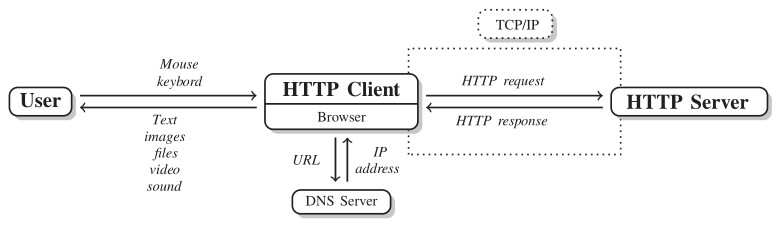
\includegraphics{images/http_schema.jpg}
\caption{\label{fig:httpschema} User-Server communication scheme via HTTP, source \citet{automateddatacollection}}
\end{figure}

Furthermore HTTP should be borne in mind two essential facts.

\begin{itemize}
\tightlist
\item
  HTTP is not only a hypertext protocol, but it is used for all sorts of services (i.e.~APIs)
\item
  HTTP is a \emph{stateless} protocol, which means that response and request and the the resulting interaction between client and server is managed by default as it were the first time they connected.
\end{itemize}

\emph{HTTP messages} consist of three sections -- start line, \emph{headers} and body -- whether client requests or server response messages. The start line of the server response begins with a declaration on the highest HTTP version. The header underneath the start line contains client and server meta data on the preferences for content displaying. Headers are arranged in a collection of name-value pairs.
The body of an HTTP message contains the content of the response and can be either binary or plain text. Predominantly in the context of the analysis are headers which are the fields where lay the definition of the actions to take upon receiving a request or response. For what concerns the analysis the focus is on \emph{identification headers} (both in request and response) whose role is to describe user preferences when sessions are opened i.e.~default language, optimization of content display throughout devices. The exploited ones are:

(metti anche altra roba da altre fonti)

\begin{itemize}
\tightlist
\item
  \emph{Authorization} (request): authentication field allows to insert personal credentials to access to dedicated content (log in to the immobiliare.it account). Credentials in requests are not really encrypted, rather they are encoded with Base64. Therefore they can be easily exposed to security breaches, which it does not happen when using HTTP (HTTP Security) that applies encryption to basic authentication, extensively presented in \ref{HTTPS}.
\item
  \emph{Set-Cookie} (response): Cookies allow the server to keep user identity. They are a method to transform \emph{stateless HTTP} communication (second point in previous ) into a secure discussion in which potential answers rely on past talks.
\item
  \emph{User-Agent} (request), faced in next section \ref{spoofing}.
\end{itemize}

\hypertarget{spoofing}{%
\subsection{User Agent and further Identification Headers Spoofing}\label{spoofing}}

\begin{definition}[User Agents]
\protect\hypertarget{def:useragents}{}{\label{def:useragents} \iffalse (User Agents) \fi{} }The user Agent (from now on refered as UA) ``retrieves, renders and facilitates end-user interaction with Web content'' \citep{UaDef}.
\end{definition}

In the HTTP identification headers the UA string is often considered as \emph{content negotiator} \citep{wiki:UserAgent}. One the basis of the UA, the web server can negotiate different CSS loadings, custom JavaScript delivery or it can automatically translate content on UA language preferences \citep{whoishostingthis.com}.
UA is a dense content string that includes many User details: the user application or software, the operating system (and versions), the web client, the web client's version, as well as the web engine responsible for content displaying (e.g.~AppleWebKit). When the request is sent from an application software as R (no web browser), the default UA is set as:

\begin{lstlisting}
## [1] "libcurl/7.64.1 r-curl/4.3 httr/1.4.2"
\end{lstlisting}

Indeed when a request comes from a web browser a full UA example and further components breakdown is (current machine):

\passthrough{\lstinline!Mozilla/5.0 (Windows NT 6.3; WOW64) AppleWebKit/537.36 (KHTML, like Gecko) Chrome/45.0.2454.85 Safari/537.36!}

\begin{itemize}
\tightlist
\item
  The browser application is Mozilla build version 5.0 (i.e.~`Mozilla-compatible').
\item
  The Operating System is Windows NT 6.3; WOW64, running on Windows.
\item
  The Web Kit provides a set of core classes to display web content in windows \citep{UserAgen23}, build version 537.36.
\item
  The Web Browser is Chrome version 45.0.2454.85.
\item
  The client is based on Safari, build 537.36.
\end{itemize}

The UA string is also one of the main responsible according to which Web crawlers and scrapers through a dedicated name field in robotstxt \ref{best-practices} may be ousted from accessing certain parts of a website. Since many requests are sent the web server may encounter insistently the same UA (since the device from which they are sent is the same) and as consequence it may block requests associated to the own UA. In order to avoid server block the scraping technique adopted in this analysis rotates a pool of UAs. That means each time requests are sent a different set of headers are drawn from the pool and then combined. The more the pool is populated the larger are the UA combinations. The solution proposed tries in addition to automatically and periodically resample the pool as soon as the website from which U agents ID are extracted updates newer UA strings.

\begin{lstlisting}[language=R]
set.seed(27)
url = "https://user-agents.net/"
agents = read_html(url) %>% html_nodes(css = ".agents_list li") %>% html_text()

agents[sample(1)]
\end{lstlisting}

\begin{lstlisting}
## [1] "Mozilla/5.0 (Windows NT 10.0; WOW64; Trident/7.0; rv:11.0) like Gecko/DCPMSY23-57"
\end{lstlisting}

The same procedure has been applied to the From identification header attached to the request. E-mails, that are randomly generated from a website, are scraped and subsequently stored into a variable. A further way to imagine what this is considering low level API calls to dedicated servers nested into a more general higher level API.
However UA field name technology has been recently sentenced as superseded in favor of a newer (2020) proactive content negotiator named \emph{Hints} \citet{wiki:UserAgentHints}.

An even more secure approach may be accomplished rotating proxy servers between the back and forth sending-receiving process.
\begin{definition}[Proxy Server]
\protect\hypertarget{def:proxy}{}{\label{def:proxy} \iffalse (Proxy Server) \fi{} }A proxy server is a gateway between the web user and the web server.
\end{definition}
While the user is exploiting a proxy server, internet traffic in the form of HTTP request, figure \ref{fig:proxycommunication} flows through the proxy server on its way to the HTTP server requested. The request then comes back through that same proxy server and then the proxy server forwards the data received from the website back to the client.
Form a user perspective benefits regards:

\begin{itemize}
\tightlist
\item
  anonymity on the Web
\item
  overcome restriction access to IPs imposed to requests coming from certain locations
\end{itemize}

Many proxy servers are offered as paid version. In this particular case security barrijers are not that high and this suggests to not apply them. As a further disclaimer many online services are providing free proxies server access, but this comes at a personal security cost due to a couple of reasons:

\begin{figure}
\centering
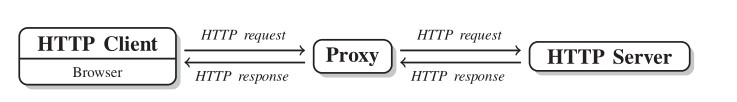
\includegraphics{images/proxy_schema.jpg}
\caption{\label{fig:proxycommunication} proxy middle man,, source \citet{automateddatacollection}}
\end{figure}

\begin{itemize}
\tightlist
\item
  Free plan Proxies are shared among a number of different clients, so as long as someone has used them in the past for illegal purposes the client is indirectly inheriting their legal infringements.
\item
  Very cheap proxies, for sure all of the ones free, have the activity redirected on their servers monitored, profiling in some cases a user privacy violation issue.
\end{itemize}

\hypertarget{possibly}{%
\section{Dealing with failure}\label{possibly}}

During scraping many difficulties coming from different source of problems are met. Some of them may come from the website's layout changes (\ref{ProperScraping}), some of them may regard internet connection, some other may have been caused by security breaches (section \ref{spoofing}).
One of the most inefficient event it can happen is an unexpected error thrown while sending requests that causes all the data acquired and future coming going lost. In this particular context is even more worrying since scraping ``main'' functions is able to call 34 different functions each of which points to a different data location. Within a single function invocation, pagination contributes to initialize 10 pages. Each single page includes 25 different single links (\ref{crawling}) leading to a number of 8500 single data pieces. Unfortunately the probability given 8500 associated to one piece being lost, unparsed is frankly high.
For all the reasons said scraping functions needs to deal with the possibility to fail. This is carried out by the implementation of \passthrough{\lstinline!purrr!} vectorization function \passthrough{\lstinline!map!} (and its derivatives) and the adverb \passthrough{\lstinline!possibly!} \citet{possibly}. \emph{Possibly} takes as argument a function (map iteration over a list) and returns a modified version. In this case, the modified function returns an empty dataframe regardless of the error thrown. The approach is strongly encouraged when functions need to be mapped over large objects and time consuming processes as outlined in \citet{Rdatascience} section 21.6. Moreover vecrotizaion is not only applied to a vector of urls, but also to a set of functions defined in the environemnt.

\begin{figure}
\centering
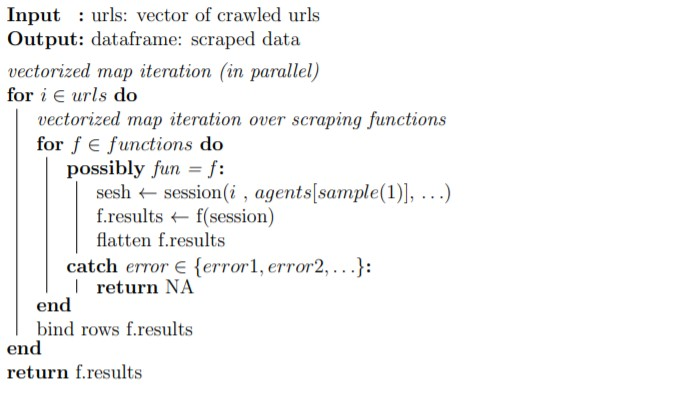
\includegraphics[width=0.7\textwidth,height=\textheight]{images/pseudocode_latex/pseudocode_possibly.jpg}
\caption{\label{fig:pseudocode2}pseudo code for a generic set of functions applied with possibly fail dealers , author's source}
\end{figure}

\hypertarget{parallelscraping}{%
\section{Parallel Scraping}\label{parallelscraping}}

Scraping run time is crucial when dealing with dynamic web pages. This assumption is stronger in Real Estate rental markets where time to market is a massive competitive advantage.
From a run time perspective the dimension of the problem requires as many html session opened as single links crawled (refer to previous section \ref{possibly}). As a result computation needs to be \emph{parallelized} in order to be feasible.
The extraordinary amount of time taken in a non-parallel environment is caused by R executing scraping on a single processor \emph{sequentially} url-by-url in a queue, left part of figure \ref{fig:singlethreaded} (i.e.~single threaded computing).

\begin{definition}[parallel]
\protect\hypertarget{def:parallel}{}{\label{def:parallel} \iffalse (parallel) \fi{} }\emph{Parallel execution} is characterized as multiple operations taking place over overlapping time periods. \citep{eddelbuettel2020parallel}
\end{definition}

This requires multiple execution units and modern processors architecture provide multiple cores on a single processor and a way to redistribute computation (i.e.~multi threaded computing). As a result tasks can be split into smaller chunks over processors and then multiple cores for each processor, right part of figure \ref{fig:singlethreaded}.
Therefore Parallel scraping (sometimes improperly called \href{https://medium.com/@cummingsi1993/the-difference-between-asynchronous-and-parallel-6400729fa897}{asynchronous}) functions are proposed, so that computation do not employ vast cpu time (i.e.~cpu-bound) and space.

\begin{figure}
\centering
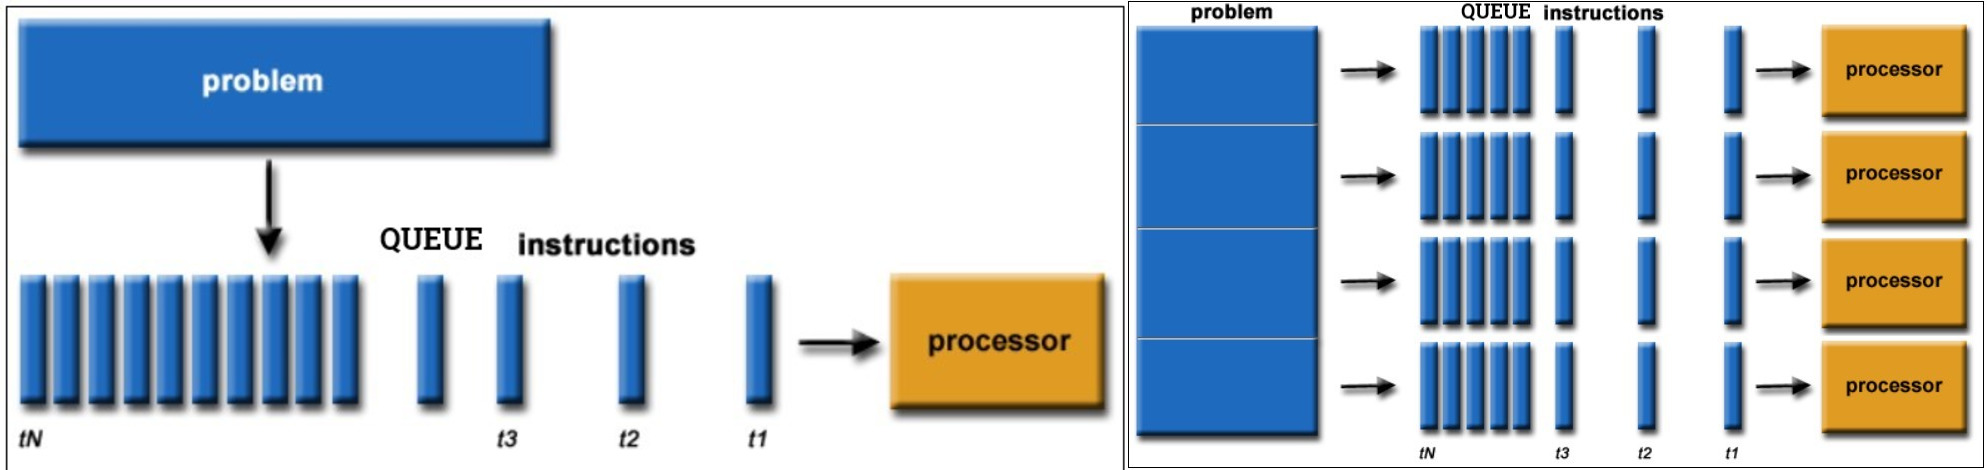
\includegraphics{images/parallel_problem.jpg}
\caption{\label{fig:singlethreaded}single threaded computing vs parallel computing, \citet{barney} source}
\end{figure}

Parallel execution heavily depends on hardware and software choice. Linux environments offers multi-core computation through \emph{forking} \citep{wiki:forking} (only on Linux) so that global variables are directly inherited by child processes. As a matter of fact when computation are split over cores they need to import whatever it takes to be carried out, such as libraries, variables, functions. From a certain angle they need to be treated as a containerized stand-alone environments. This can not happen in Windows (local machine) since it does not support multicore.

\begin{lstlisting}[language=R]
future::supportsMulticore()
\end{lstlisting}

\begin{lstlisting}
## [1] FALSE
\end{lstlisting}

\emph{Cluster processing} is an alternative to multi-core processing, where parallelization takes place through a collection of separate processes running in the background. The parent R session instructs the dependencies that needs to be sent to the children sessions.
This is done by registering the parallel back end. Arguments to be supplied mainly regards the strategy (i.e.~multi-core cluster, also said multisession) and the \emph{working group}. The working group is a software concept \citep{parallelr}, that points out the number of processes and their relative computing power/memory allocation according to which the task is going to be split. Moreover from a strictly theoretic perspective the \emph{workers} (i.e.~working group single units) can be greater than the number of physical cores detected. Although parallel libraries as a default choice (and choice for this analysis) initializes \emph{as many workers as} physical HT (i.e.~Hyper Threaded) \emph{cores}.
Parallel looping constructor libraries generally pops up as a direct cause of new parallel packages. The latest research activity by Bengtsson \citet{doFuture} indeed tries to unify all the previous back ends under the same umbrella of \passthrough{\lstinline!doFuture!}. The latter library allows to register many back ends for the most popular parallel looping options solving both the dependency inheritance problem and the OS agnostic challenge.
The two alternatives proposed for going parallel are \passthrough{\lstinline!Future!} \citet{future} with \passthrough{\lstinline!furrr!} \citet{furrr} and \passthrough{\lstinline!doFuture!} \citeyearpar{doFuture} along with the \passthrough{\lstinline!foreach!} \citet{foreach} loop constructor. The former is a generic, low-level API for parallel processing as in \citet{bengtsson_2017}. The latter takes inspiration by the previous work and it provides a back-end agnostic version of \passthrough{\lstinline!doParallel!} \citet{doParallel}.
Further concepts on parallel computing are beyond the scope of the analysis. However they can be explored in \citet{barney}, which may offers a comprehensive perspective on Parallel theory both on hardware and software. Indeed for a full reference on the R parallel ecosystem, run time simulations and advanced algorithm back end design strategies, the authorities are \citet{parallelr}. If the interest is to cut short theory and directly put existing R code into parallel, a valuable resource is covered in \href{https://nceas.github.io/oss-lessons/parallel-computing-in-r/parallel-computing-in-r.html}{blog}, which also investigate the main debugging aspects.

\hypertarget{parallel-furrrfuture}{%
\subsection{Parallel furrr+future}\label{parallel-furrrfuture}}

\textbf{cerca di centrare di più su scraping}

Simulations are conducted on a not-rate-delayed (section \ref{best-practices}) and restricted set of functions which may be considered as a ``lightweight'' version of the final API scraping endpoint.
As a disclaimer run time simulations may not be really representative to the problem since they are performed on a windows 10, Intel(R) Core(TM) i7-8750H 12 cores RAM 16.0 GB local machine. Indeed the API is served on a Linux Ubuntu distro t3.micro 2 cores RAM 1.0 GB server which may adopt forking. Simulations for the reasons said can only offer a run time performance approximation for both of the parallel + looping constructor combinations.

The first simulation considers \passthrough{\lstinline!furrr!} which enables mapping (i.e.~vectorization with \passthrough{\lstinline!map!}) through a list of urls with \passthrough{\lstinline!purrr!} and parallelization with \passthrough{\lstinline!Future!}. Future gravitates around a programming concept called ``future'', initially introduced in late 70's by Baker \citep{BakerFuture}. Futures are abstractions for values that may be available at a certain time point later \citeyearpar{future}.
These values are result of an evaluated expression, this allows to actually divide the assignment operation from the proper result computation. Futures have two stages \emph{unresolved} or \emph{resolved}. If the value is queried while the future is still unresolved, the current process is blocked until the stage is resolved. The time and the way futures are resolved massively relies on which strategy is used to evaluate them. For instance, a future can be resolved using a \emph{sequential} strategy, which means it is resolved in the current R session. Other strategies registered with \passthrough{\lstinline!plan()!}, such as \emph{multi-core} (on Linux) and \emph{multisession}, may resolve futures in parallel, as already pointed out, by evaluating expressions on the current machine in forked processes or concurrently on a cluster of R background sessions.
With parallel futures the current/main R process does not get ``bottlenecked'', which means it is available for further processing while the futures are being resolved in separate processes running in the background. Therefore with a ``multisession'' plan are opened as many R background sessions as workers/cores on which chunks of futures (urls) are split and resolved in parallel. From an algorithmic point of view It can be compared to \emph{a divide and conquer} strategy where the target urls are at first redistributed among workers/cores (unresolved) through background sessions and then are scraped in equally distributed chunks (resolved).
Furthermore furrr has also a convenient tuning option which can interfere with the redistribution scheduling of urls' chunks over workers. The argument scheduling can adjust the average number of chunks per worker. Setting it equal to 2 brings \emph{dinamicity} \citeyearpar{furrr} to the scheduling so that if at some point a worker is busier then chunks are sent to the more free ones.

(migliore rappresentazione)

\begin{figure}
\centering
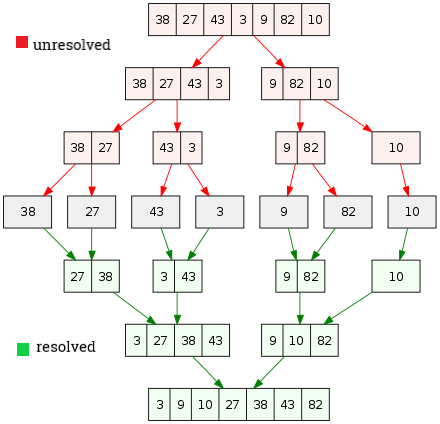
\includegraphics{images/divideconquer.png}
\caption{\label{fig:divideconquer}futures reimagined as divide and conquer, author's source}
\end{figure}

The upper plot in figure \ref{fig:furrrfuture} are 20 simulations of 100 url (2500 data points) performed by the lightweight scraping. On the x-axis are plotted the 20 simulations and on the y-axis are represented the respective elapsed times. One major point to breakdown is the first simulation run time measurement which is considerably higher with respect to the others i.e.~15 sec vs mean 7.72 sec.~Empirical demonstrations traces this behavior back to the opening time for all the background sessions. As a result the more are the back ground sessions/workers, the more it would be the time occupied to pop up all the sessions. As opposite whence many sessions are opened the mean execution time for each simulation is slightly less.
The lower plot in in figure \ref{fig:furrrfuture} tries to capture the run time slope behavior of the scraping function when urls (1 to 80) are cumulated one by one. The first iteration scrapes 1 single url, the second iteration 2, the third 3 etc. Three replications of the experiment has been made, evidenced by three colours. The former urls are more time consuming confirming the hypothesis casted before. Variability within the first 40 urls for the three repetitions does not show diversion. However It slightly increases when the 40 threshold is trespassed. Two outliers in the yellow line are visible in the nearby of 50 and 60. It can be assumed that workers in that urls neighbor may be overloaded but no evidences are witnessed on cores activity as in plot \ref{fig:cpumonitor}. The measured computational complexity of scraping when \(n\) is number of urls seems to be much more less than linear \(\mathcal{O}(0.06n)\).

\begin{figure}
\centering
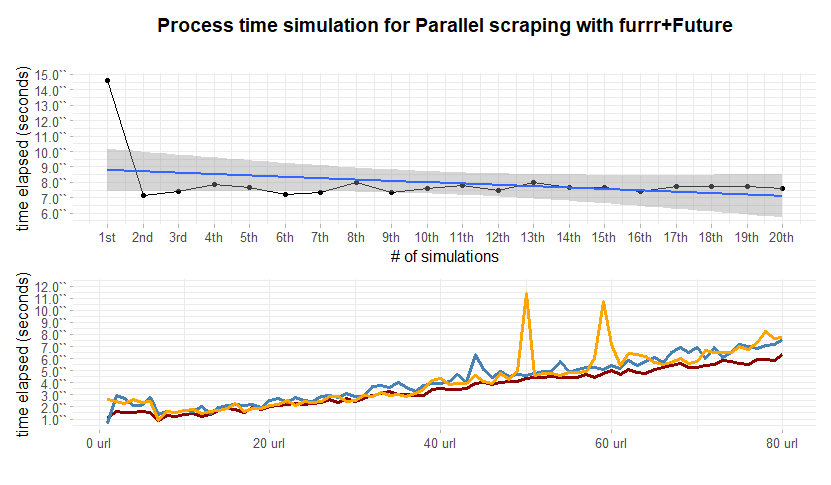
\includegraphics{images/simulations/final_furrr_future.png}
\caption{\label{fig:furrrfuture}computational complexity analysis with Furrr}
\end{figure}

\begin{figure}
\centering
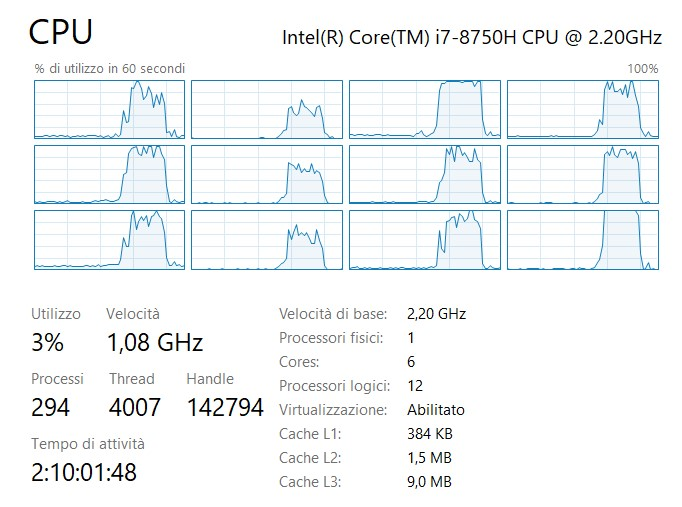
\includegraphics{images/parallel_computing.jpg}
\caption{\label{fig:cpumonitor}local machine monitoring of cores during parallel scraping}
\end{figure}

\hypertarget{parallel-foreachdofuture}{%
\subsection{Parallel foreach+doFuture}\label{parallel-foreachdofuture}}

A second attempt tries to encapsulate \passthrough{\lstinline!foreach!} \citep{foreach} originally developed by Microsoft R, being a very fast loop alternative, parallelized with \passthrough{\lstinline!doFuture!}. The package registered with older back ends required rigorous effort to specify exact dependencies for child process inside foreach arguments \passthrough{\lstinline!.export!}. From a certain angle the approach could led to an indirect benefit from memory optimization. If global variables needs to be stated than the developer might be forced to focus on limiting packages exporting. Indeed since doFuture implements optimized auto dependency search this problem may be considered solved as in \citet{doFuture}. Two major looping related speed improvements may come from \passthrough{\lstinline!.inorder!} and \passthrough{\lstinline!.multicombine!} arguments which both take advantage of parallel split disorder a subsequent recombination of results. In the context where data collection order matters this is extremely wrong, but since in this case order is defined through url composition based on criteria expressed inside nodes contents this can be totally applied. A drawback of enabling .multicombine is a worst debugging experience since errors are thrown at the end when results are reunited and no traceback of the error is given.

The upper part in \ref{fig:foreachdofuture} displays lower initialization lag from R sessions opening and parallel execution that also lead to a lower mean execution time of 6.42 seconds. No other interesting behavior are detected.
THe lower plot displays high similarities with the curves in \ref{fig:furrrfuture} highlighting an outlier in the same proximities of 45/50 urls. The blue simulation repetition shows an uncommon pattern that is not seen in the other plot. Segmented variability from 40 to 80 suggests a higher value which may be addressed do instability. As a result the approach is discarded in favor of furrr + future which also offers both a comfortable \{Tidyverse\} oriented framework and offers and easy debugging experience.

\begin{figure}
\centering
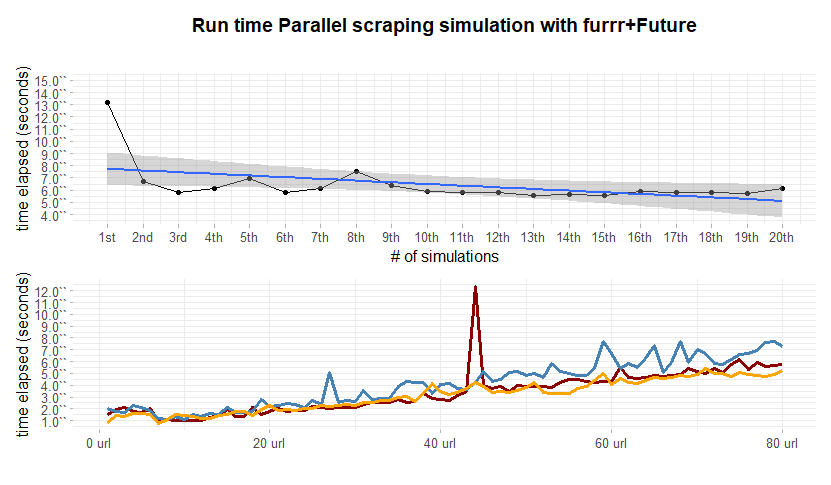
\includegraphics{images/simulations/final_foreach_dofuture.png}
\caption{\label{fig:foreachdofuture}computational complexity analysis with Furrr}
\end{figure}

\hypertarget{challenges}{%
\section{Open Challenges and Further Improvemements}\label{challenges}}

Although results are quite encouraging still one of the main challenges remains unsolved. In fact optimization has involved each scraping layer but scraping function must be continuously kept up with the immobiliare.it changes, particularly the crawling part. Indeed the proper scraping part, with some further adjustments can take care of auto-search for exact information within the web page even if the design changes. This idea is massively applied in the package Rcrawler \citet{Rcrawler}, which doesn't apply segmentation in crawling, instead it downloads the entire website and then inspects targeted keywords. The major benefit relies in crawling HTML/XML that are agreed to be generally lightweight in this way the process does not weigh down the run time.
Whence all files are saved locally the algorithm applies search methodologies within the HTML files. Run time performance with algorithm of this kind with respect to the amount of data gathered are very efficient, nevertheless results are not always effective due to keywords disambiguation.
Afterall a way safer and time saving approach to general scraping may be including complex theme specific regular expressions on the HTML text which univocally identify CSS data location. With that said the idea would be an unsupervised algorithm that combines the traditional browser search + a selector gadget for CSS conversion.
As a disclaimer Rcrawler is designed to be flexible to scrape a vast number of websites. As opposite the scraping functions here presented are exclusively built on top of immobiliare.it, even though they can be extended with a small effort to other category related website \ref{webstructure}.
On the parallel computing side a further boosts might be added with parallel distributed processing through HPC (high-performance computing) clusters by \passthrough{\lstinline!future.batchtools!} \citet{futurebatchtools}. The package implements a generic future wrapper around batchtools with job scheduler like Torque, Slurm, Sge and many more. A higher level API built on top of the Future framework that exploits \href{https://cloudyr.github.io/googleComputeEngineR/articles/massive-parallel.html}{Google Cloud Engine Clusters} i.e.\passthrough{\lstinline!cloudyR!} allows to distribute computation on Google machines.

\hypertarget{legal-profiles}{%
\section{Legal Profiles}\label{legal-profiles}}

There is a legitimate \emph{gray} web scrapers area, not only creating possible new uses for the data collected, but also potentially damaging the host website \citep{WhatCour57}. Online platforms and the hunger for new data insights are increasingly seeking to defend their information from web scrapers. Online platforms are unfortunately not always successful distinguishing users between polite, impolite and criminals, risking new ones Valid competition and creativity. A minimal but effective self limitation can really be
The courts have fought hard to achieve clear judgments Cases for web scraping. The crucial obstacle is a coherent verdicts to ascertain ``Kitchen Sink'' \citep{Kitchens81}, the standard web claim discontroversy on scraping. Kitchen Sink main arguments are:

\begin{itemize}
\tightlist
\item
  Legal lawsuits under the Computer Fraud and Abuse Act (CFAA) allegation that the defendant ``overtook'' allowed access \emph{miss lit}
\item
  Copyright infringement charges under the Digital Millennium Act or federal copyright law Copyright laws \emph{miss lit}
\item
  ``state trespass to chattels claims'' \emph{miss lit}
\item
  Contract agreements terms violation claims
\end{itemize}

A second challenge to clear verdicts is that there are several purposes for which a business model operates in a continuum of social acceptability hiring web scrapers \citep{ADetaile90}. As an example Googlebot ranks, sorts and indexes search results for Google users, without which the search would not optimized and business would not profit from this fact. A more coherent case is represented by the exploitation of scraping on online Real Estate advertiser whose importance is ascertained by the fact that they are the fist house purchase media 52\% (USA survey) and searches are expected to be growing by 22\% per yeay \citep{peterson2003consumer}. On the other hand it is estimated that the 20\% of crawlers are actually DoSsing scrapers \citep{TheInter5} causing an economic damage, as in \ref{DoS}. Unfortunately the majority of web scraping services fall between these two extremes \citeyearpar{WhatCour57}.
The most discussed and observed case regards Linkedin Corp.~``Linkedin'' vs hiQ Labs Inc.~(``hiQ'') whose claim argues the exploitation of the former personal profile data to offer a series of HR services. The litigation started by accusing hiQ with ``using processes to improperly, and without authorization, access and copy data from LinkedIn's website'' \citep{Letterfr71}. As reinforcement to their arguments they presented also a citation directly form their terms raising the point on copying, web scarping prohibition without their explicit consent. Furthermore Linkedin noted that technical barriers were taken into existence to restrict the access of hiQ to the platform and warned of a breach of state and federal law by ignoring such barriers \citeyearpar{WhatCour57}. As a response Hiq submitted a temporary restricting order to prevent LinkedIn from denying the access to their platform, focusing on the aspect that the motivation was led by an anticompetitive intent. Linkedin's response brought into the litigation CFAA which actually pollutes argumentation since Court evidences that CFAA is ambiguous whether it is granting or restringing the access to public available website \citep{hiQLabsI66}. In other words CFAA intent was to protect user data when they are authenticated with passwords, and in no case out of these borders. In the end the litigation moved to the Ninth Circuit where in 2019 it uphelds the preliminary injunction to prohibit LinkedIn from continuing to provide access to publicly accessible LinkedIn member profiles to the claimant hiQ Labs \citep{wiki:HiQvsLinkedIn}.
Immobiliare.it expressed similarly to linkedin in their terms \citep{immobiliareterms} the prohibition to reproduce any form of intellectual property in their web pages. This once again does not imply the inaccessibility to scraping their content and should not in any case prevent the usage of an open sourced tool inspired by research grounds and efficient market choices.

\hypertarget{Infrastructure}{%
\chapter{API Technology Stack}\label{Infrastructure}}

The previous chapter has encapsulated the main concepts behind the design of consistent, secure, and fast scraping functions with R. In truth challenges not only regard scraping per se, but also the way and how many times the service has to interact with different clients. Indeed the fact that functions are compressed into scripts does not imply that are shareable and portable. As a consequence when they are executed they also need to be at first understood and secondly loaded into a dedicated R environment (higher and lower dependecies). Moreover results are actually computed, whether in parallel or not, with local machines resources that are limited in many sense. In the end exposing the service traffic to the public or internally to a network of servers requires authentication and precautions from both malicious attack and privacy dangers. Actually from a restricted personal usage perspective what has been done since now is totally feasible. But in a large-scale orientation where different stakeholders should gather massive amount of data, then a unsuitable service may cause an enormous waste of time.
The following chapter tries to capture the essence and its specific context usage of each technology involved that address each aforementioned issues raised. In parallel it highlights the \emph{fil rouge} that ties together the chronological order according to which the stack has been developed.

The recipe proposed serves a REST Plumber API (an R framework) with 2 endpoints each of which calls Parallel scraping functions accomodated in section \ref{scraping}. Precautions regards sanitization of user inputs, anti-Dossing strategies and log monitoring. The software enviroment is containerized in a Docker container and \emph{Composed} with a further container housing NGINX proxy server. Orchestration is managed with docker compose. NGINX with SSL certificates bring HTTPS communication and authentication. An AWS free tier EC2 server hosts the orchestation of containers and the IP is made Elastic. Furthermore the software development is made automatic with a straightforward composition of cloud services that ignites sequential building when local changes are pushed to cloud repository.

Technology stack:

\begin{itemize}
\tightlist
\item
  GitHub version control and CI
\item
  Plumber REST API, section \ref{plumberapi}
\item
  Docker containers and compose, section \ref{docker}
\item
  NGINX reverse proxy, section \ref{nginx}
\item
  HTTPS and SSL certificates \ref{HTTPS}
\item
  AWS EC2 \ref{aws}
\end{itemize}

\textbf{immagine infrastruttura da rivedere}

\begin{figure}
\centering
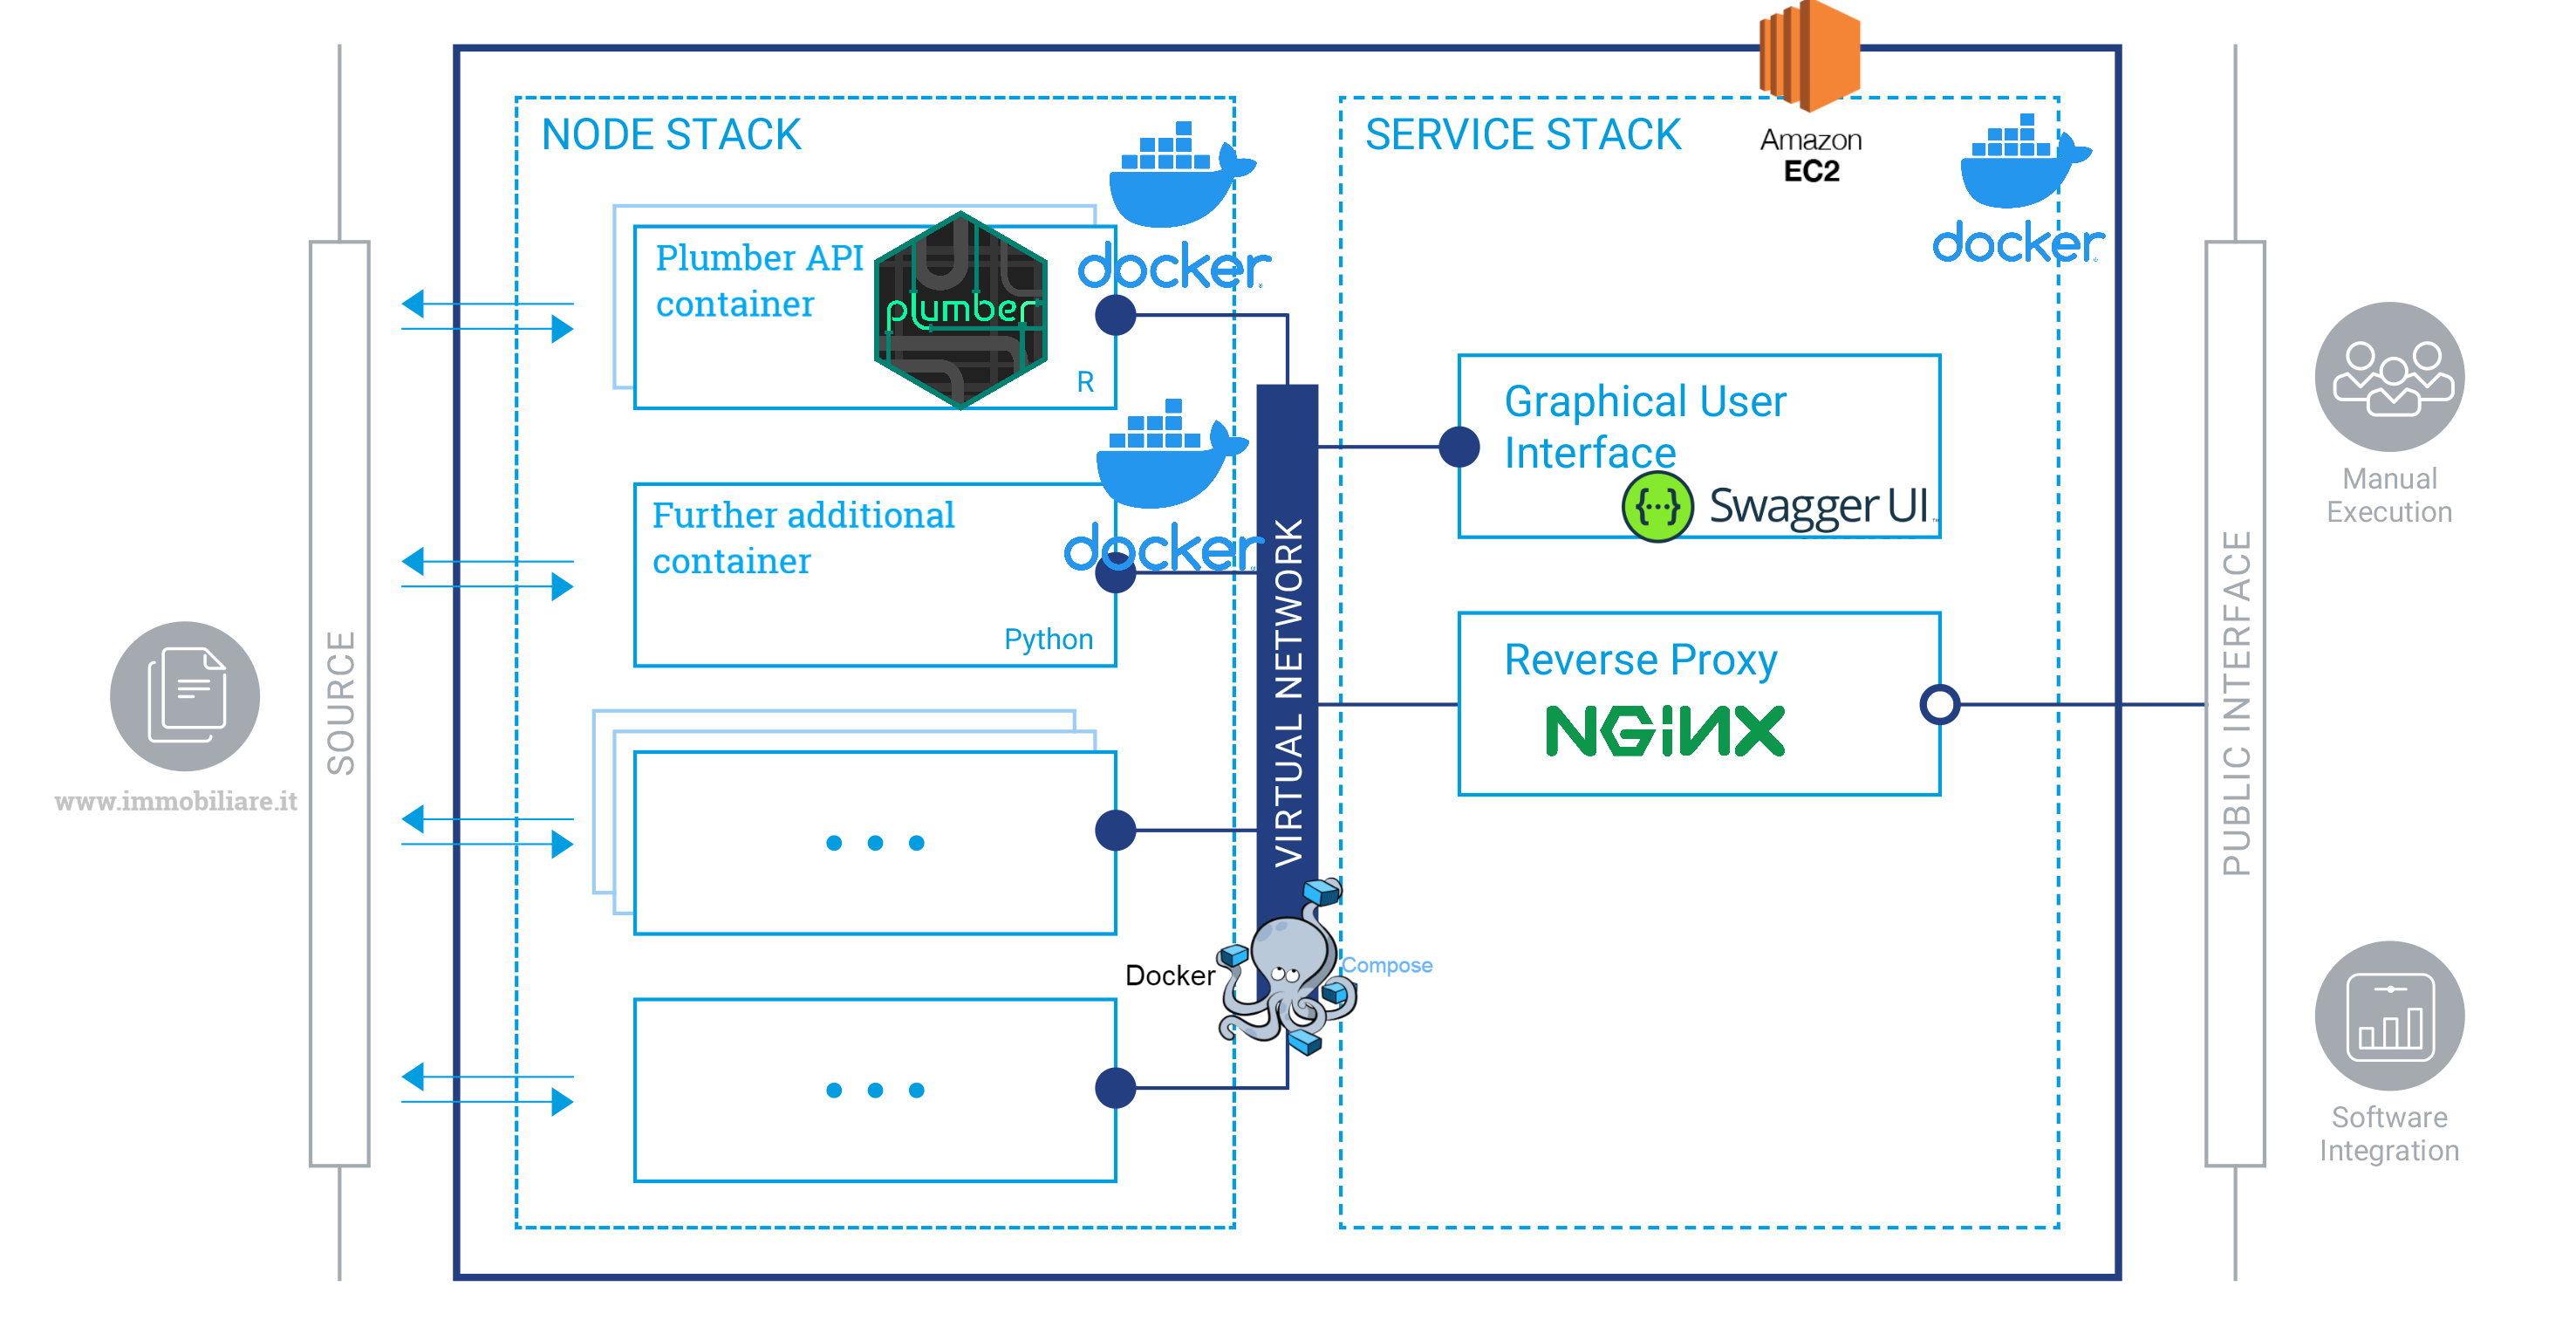
\includegraphics{images/software_arch.jpg.png}
\caption{\label{fig:CompleteStructure}complete infrastructure, author's source}
\end{figure}

As a further note each single part of this thesis is comprised according to the service inspiring criteria of portability and self containerization. RMarkdown \citep{rmarkdown1} documents (book's chapters) are knitted and then rendered as .html files extension through Bookdown \citep{bookdown2}. The resulting .html documents are instructed by a .yml file and then are rendered as Gitbook format. Gitbooks are interactive online documentation that are employed to build books, technical documentation as well as research papers. That makes thesis' graphs and codes interactive. Moreover Gitbooks enables custom buttons to directly create a push request on documents from source, which may be convenient for continous review. It is able to directly share documents on social media, as well as to change the the documents' style, such as fonts and background color.\\
Files are ultimately pushed into a \href{https://github.com/NiccoloSalvini/thesis}{Github repository}, that enables thesis version controlling. By a simple trick with GH pages a new branch is opened. .html files are displayed into a sub domain repository hosted at \href{https://niccolosalvini.github.io/thesis/}{link}, as a consequence thesis is also linked online. Moreover the Gitbook is able to produce also a .pdf version output through a Xelatex engine. Xelatex compiles .Rmd documents according to formatting rules contained in both a .tex template and a further .ylm and produces the final .pdf paper output.

\hypertarget{restful-api}{%
\section{RESTful API}\label{restful-api}}

\begin{definition}[API]
\protect\hypertarget{def:api}{}{\label{def:api} \iffalse (API) \fi{} }API stands for application programming interface and it is a set of definitions and protocols for building and integrating application software. Most importantly APIs let a product or a service communicate with other products and services without having to know how they're implemented.
\end{definition}
API may be considered as a mediator between users or clients sending a request, left part figure \ref{fig:apigenstru} and the web resource or services they want (returning back a response) middle part figure \ref{fig:apigenstru}. It also acts as means of exchanging resources and knowledge with an entity, as databases left part figure \ref{fig:apigenstru} preserving protection, control and authentication, such as who gets access to what.
There are many types of APIs that exploit different media and architectures to communicate with apps or services.
\begin{definition}[REST]
\protect\hypertarget{def:rest}{}{\label{def:rest} \iffalse (REST) \fi{} }The specification REST stands for \textbf{RE}presentational \textbf{S}tate \textbf{T}ransfer and is a set of \emph{architectural principles}.
\end{definition}

If a client request is made using a REST API, a representation of the resource state is passed to a requestor or \emph{endpoint} \citep{what_is_a_rest_api}. This information is returned in one of the formats of multiple formats using \emph{HTTP}: JSON, HTML, XLT, Python, PHP or simple text. JSON is the most common programming language to use because it is language agnostic \citeyearpar{what_is_a_rest_api} and easy to interpretable both for people and machines.
REST architecture depends upon HTTP, as a matter of fact REST API inherits from HTTP the stateless property, second pillar in \ref{HTTPmethod}. Calling a REST API (producing a request) demands composing a well defined URL lower part in figure \ref{fig:apigenstru}, whose semantic is able to uniquely identify the resource or a group of resources (sending back a response) along with the most common HTTP methods, as GET, PUT, POST, DELETE.

\begin{figure}
\centering
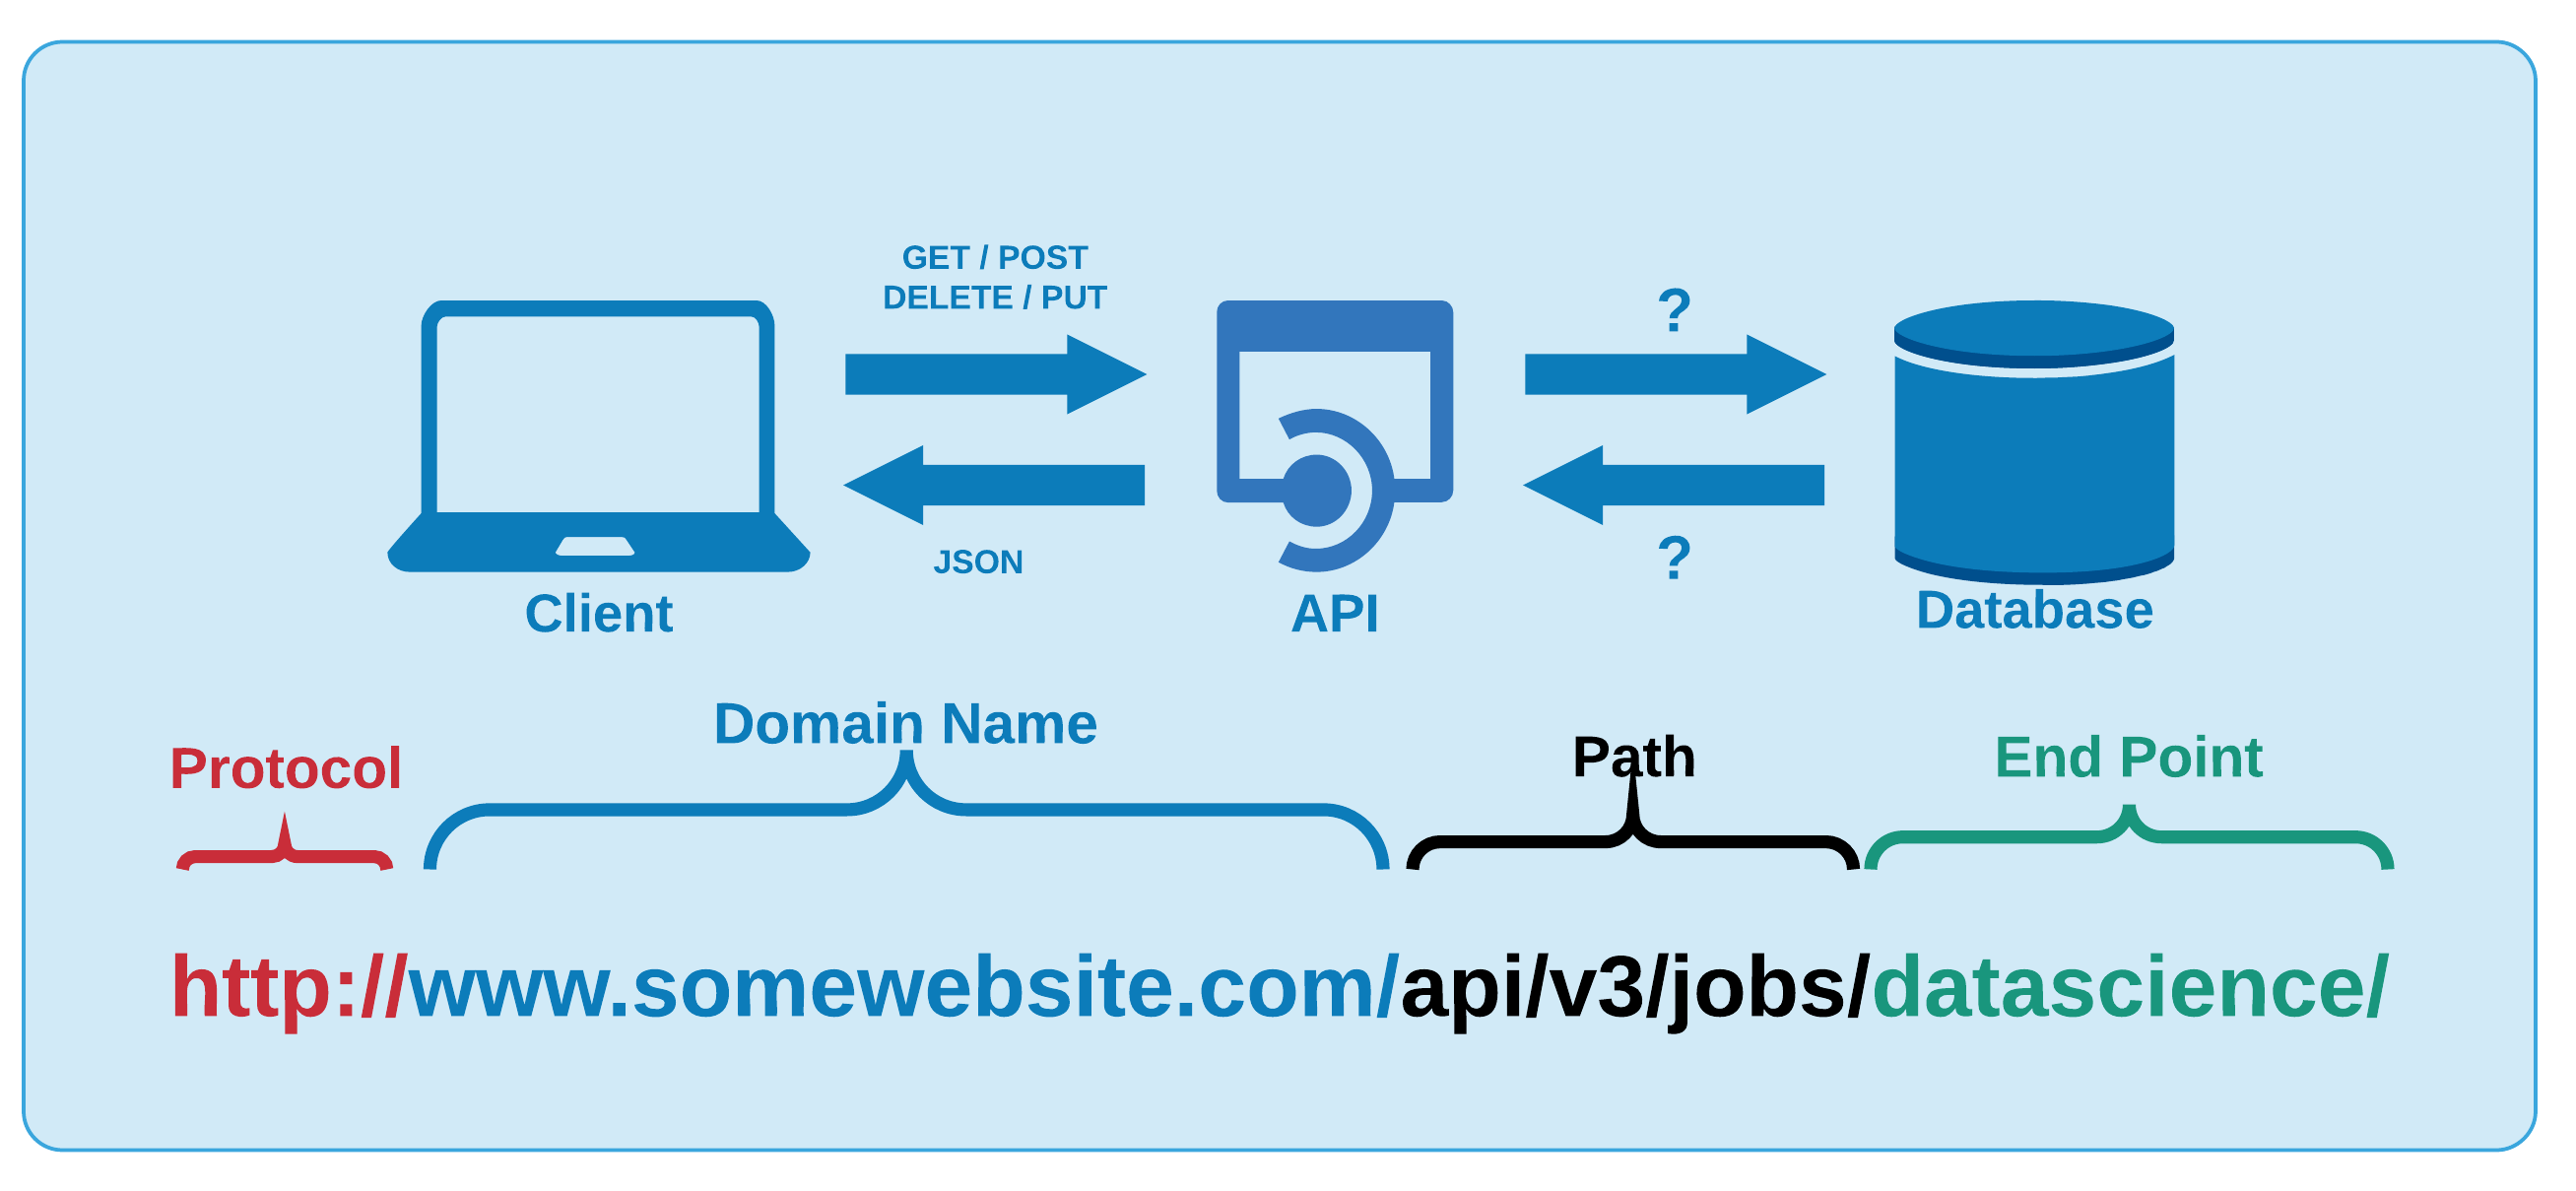
\includegraphics{images/api_stru.png}
\caption{\label{fig:apigenstru}API general functioning, unknown source}
\end{figure}

When an API adheres to REST \ref{def:rest} principles is said RESTful. Principles are:

\begin{itemize}
\tightlist
\item
  A client-server architecture made up of clients, servers, and resources, with requests managed through HTTP method.
\item
  Stateless client-server communication, meaning no client information is stored between requests and each request is separate and disconnected.
\item
  Cacheable data that streamlines client-server interactions.
\item
  A uniform interface between components so that information is transferred in a standard form. This requires that:

  \begin{itemize}
  \tightlist
  \item
    resources requested are identifiable and separate from the representations sent to the client.
  \item
    resources can be manipulated by the client via the representation they receive because the representation contains enough information to do so.
  \item
    self-descriptive messages returned to the client have enough information to describe how the client should process it.
  \end{itemize}
\item
  A layered system that organizes each type of server (those responsible for security, load-balancing, etc.) involved the retrieval of requested information into hierarchies, invisible to the client.
\end{itemize}

RESTful APIs receives HTTP request inputs and elaborates them through endpoints. Endpoints are the final step in the process of submitting an API request and they can interpreted as the responsibles for generating a response \citeyearpar{plumber}. Further documentation and differences between HTTP and REST API can be found to this \href{https://docs.aws.amazon.com/it_it/apigateway/latest/developerguide/http-api-vs-rest.html}{reference}.
Open and popular RESTful API examples are:

\begin{itemize}
\tightlist
\item
  BigQuery API: A data platform for customers to create, manage, share and query data.
\item
  YouTube Data API v3: The YouTube Data API v3 is an API that provides access to YouTube data, such as videos, playlists, and channels.
\item
  Skyscanner Flight Search API: The Skyscanner API lets you search for flights \& get flight prices from Skyscanner's database of prices, as well as get live quotes directly from ticketing agencies.
\item
  Openweathermap API: current weather data for any location on Earth including over 200,000 cities.
\end{itemize}

\hypertarget{plumberapi}{%
\subsection{Plumber HTTP API}\label{plumberapi}}

Plumber is a R framework \citep{an_api_generator_for_r}, allowing users to construct HTTP APIs simply by adding decoration comment to the existing R code, in this context to scraping code. Decorations are a special type of comments that suggests to Plumber where and when the API specifications start. Below is reported a toy API with 3 endpoints inspired by the original documentation. Endpoints in the following code chunk are identifiable by the three distinguishing comment blocks, separated by the aforementioned decorations. http API specifications require the user to set the endpoint description (first comment), to specify the parameters role and input type (second), and the http method i.e.~GET, POST followed by the endpoints invokation verb e.g.~echo, plot, sum (third).

\begin{lstlisting}[language=R]
# plumber.R

#* Echo back the input
#* @param msg The message to echo
#* @get /echo
function(msg="") {
  list(msg = paste0("The message is: '", msg, "'"))
}

#* Plot a histogram
#* @param n the number of samples
#* @serializer png
#* @get /plot
function(n = 10) {
  rand = rnorm(n = n)
  hist(rand)
}

#* Return the sum of two numbers
#* @param a The first number to add
#* @param b The second number to add
#* @post /sum
function(a, b) {
  as.numeric(a) + as.numeric(b)
}
\end{lstlisting}

Once HTTP api calls are sent to machines belonging to a single server or a network of servers, whether it is public or private they converge through endpoints. Endpoints execute functions involving the parameters specified through the call and by default response is JSON type. The first endpoint ``echo'' invocation simply \emph{echoes} back the text that it was sent. The second endpoints generates a histogram \emph{plot} i.e.~.png file based on a Normally distributed sample whose observation number are ``n''. The third endpoint calculates the \emph{sum} of a couple of number attached to the call. Scraping function are then implemented within the API framework and arguments becomes parameters for an incoming request. Many more options may induce plumber endpoints to respond in the preferred fashion, in any case are beyond the scope of the analysis.
Exposing APIs on a private network or on a public server security is a major issue. Concerns and thought process therefore must adapt accordingly. There are several variables and consequent attacks that should be considered while creating Plumber APIs, but the focus will differ depending on the API audience. For example if APIs are offered without authentication on the Internet, potential vulnerabilities should seriously convince the api maintainer to properly account each of them. Three in the context of the analysis are critical:

\begin{itemize}
\tightlist
\item
  Sanitization
\item
  Denial Of Service (DoS)
\item
  Logging
\end{itemize}

\hypertarget{sanitize}{%
\subsection{Sanitization}\label{sanitize}}

Whenever APIs accept input from a random user this is directly injected into functions through endpoints, therefore the worst case scenario should be prepared. In the context of the analysis users are required to specify to the endpoints arguments such as cities, zones, number of pages and many others. Chances are that users might either misspell inputs or use different encoding (accents) or rather use capital letters when functions are capital sensitive. Endpoints should take account of the behavior by sanitizing whatever it comes into the function. The process at first requires an intense and creative investigation on what it can be misused and how. Then Secondly new functional inputs are defined so that they take the user generated input and give back a sanitized version inside the function. In the code chunk below are shown a couple of examples of sanitization of inputs:

\begin{lstlisting}[language=R]
tipo = tolower(type) %>% str_trim()
citta = tolower(city) %>% iconv(to = "ASCII//TRANSLIT") %>% str_trim()
macroozone = tolower(macrozone) %>% iconv(to = "ASCII//TRANSLIT") %>% str_trim()
\end{lstlisting}

Inputs make their entrance into functions through arguments ``type'', ``city'' and ``macrozone'' and are immediately preprocessed. They are in sequence converted to lower cases, then extra spaces are trimmed, in the end accents are flattened.

\hypertarget{DoS}{%
\subsection{Denial Of Service (DoS)}\label{DoS}}

Denial-of-service attacks (DoS) are used to temporarily shut down a server or service through traffic congestion. A DoS scenario could be triggered accidentally by a malicious user requesting the server for an infinite looping task. Other scenarios might depict a malicious hacker who uses a large number of machines to repeatedly make time consuming requests to occupy the server, this is the case of DDoS (Distributed Denial of Service). DoS or DDoS attacks may also induce anomalies and deprives system resources, which in the context of hosting services may result in astronomical fees charged. Dos attack as a conseuquence may also induce distorted website/API logs analytics, leading to distorted reports.
A simple but effective approach tries to limit and stop the number of request sent:

\begin{lstlisting}[language=R]
 if (npages > 300 & npages > 0){
                        msg = "Don't DoS me!"
                        res$status = 500 # code num: Bad request
                        stop(list(error=jsonlite::unbox(msg)))     
            }
\end{lstlisting}

The code chunk above intercepts DoS attacks by limiting to 300 the number of pages to be server to the API. Furthermore it converts outputs error messages printed on console into JSON format and then pass them as output. This simplify distinguishing malicious attacks from a type errors. DDoS attacks are secured by SSL certificates and Authentication covered later in the chapter.

\hypertarget{logging}{%
\subsection{Logging}\label{logging}}

Plumber uses ``filters'' that can be resorted to describe a ``pipeline'' for processing incoming request. This enables API maintainers to separate complex logic into discrete, comprehensible steps. Usually, before trying to find an endpoint that satisfies a request, Plumber passes the request through the \emph{filters}. When APIs are called, requests pass through filters one at a time and Plumber forwards i.e.~\passthrough{\lstinline!forward()!} the request to the next filter untill the endpoints. Filters applications ranges from excluding client request based on request parameters or may offer also a thin layer of authentication. Filters might also be used as a logging for requests where logging, i.e.~the act of keeping a log \citep{wiki:logging}, is recording events in an operating system or running software from other users of communication software, or messages among different subjects.
A request log filter might have this appearance:

\begin{lstlisting}[language=R]
#* Log information
#* @filter logging
function(req){
            cat(as.character(Sys.time()), "-",
                req$HTTP_USER_AGENT, "@", 
                req$REMOTE_ADDR, "\n",
                req$QUERY_STRING, "\n")
            plumber::forward()
}
\end{lstlisting}

The above filter parses the request through the default request argument \passthrough{\lstinline!req!}, then it prints out messages about the incoming User Agent (i.e.~\passthrough{\lstinline!HTTP\_USER\_AGENT!}) (section \ref{spoofing}), the \passthrough{\lstinline!REMOTE\_ADDR!} which is the IP address of the client making the request \citeyearpar{plumber} and the \passthrough{\lstinline!QUERY\_STRING!} that records the parameters directly sent the endpoint. This helps to traceback clients activity on the API as well as detecting misuse.

\hypertarget{docs}{%
\subsection{RESTful API documentation}\label{docs}}

The service disposes of 2 endpoints \emph{/fastscrape} , \emph{/completescrape}. Parameters are the same for both of the endpoints since they rely on the same reverse engineering url algorithm \ref{fig:pseudocode3}, in section \ref{reverse}. Moreover Plumber APIs are natively wrapped up around Swagger UI helping development team or end users to imagine and communicate with the resources of the API without any discharge logic \citep{swaggerUI}. The OpenAPI (formerly referred to as Swagger), with the visual documentation facilitates backend implementation and client side consumption, as well as being automatically created by the APIs specification (parameters, endpoints\ldots). Some of the major assets in Swagger UI are: The user interface works in any environment, whether locally or web and it is suited for all main browsers.

\begin{figure}
\centering
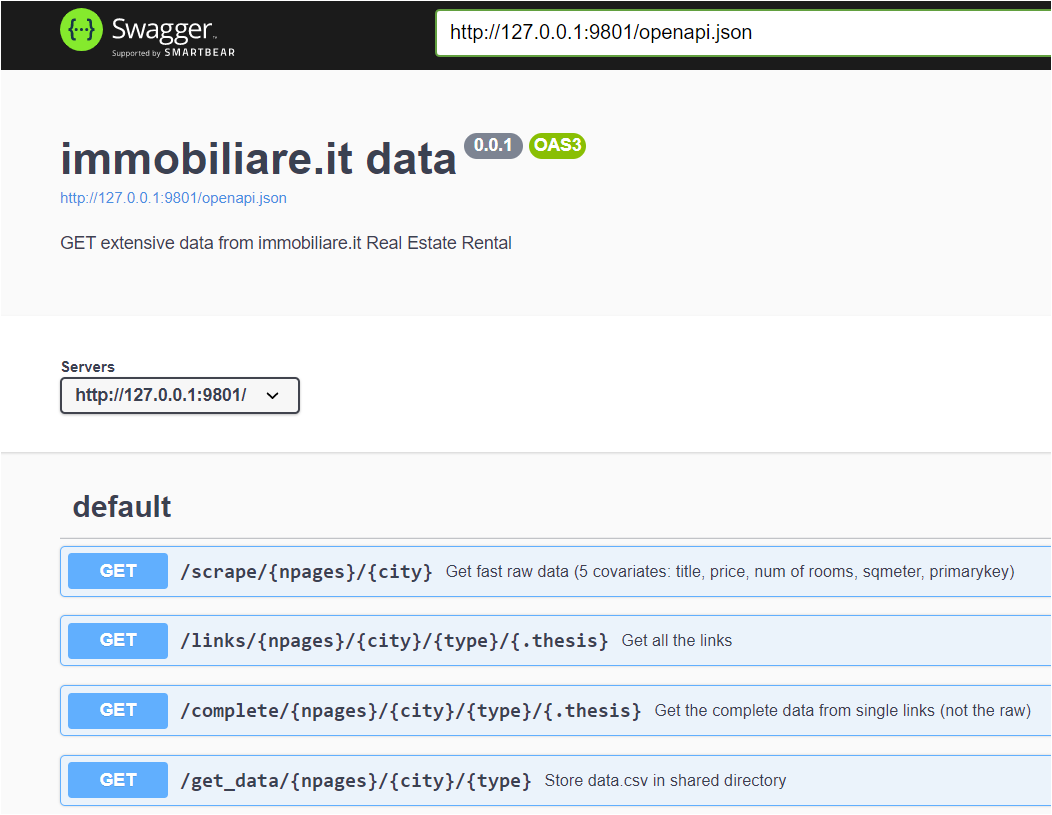
\includegraphics{images/swagger.PNG}
\caption{\label{fig:swagger}Swagger UI in localhost on port 8000, author's source}
\end{figure}

\hypertarget{docker}{%
\section{Docker}\label{docker}}

The API up to this point needs a dedicated lightweight software environment that minimizes dependencies both improving performances and enabling \emph{cloud computing} coverage. A fast growing technology known as \emph{Docker} might extend these capabilities.
\begin{definition}[Docker and Containers]
\protect\hypertarget{def:docker}{}{\label{def:docker} \iffalse (Docker and Containers) \fi{} }\emph{Docker} \citep{docker} is a software technology to create and deploy applications using containers.
\emph{Docker containers} are a standard unit of software (i.e.~software boxes) where everything needed for applications, such as libraries or dependencies can be run reliably and quickly. Containers are also portable, in the sense that they can be taken from one computing environment to the following without further adaptations.
\end{definition}
Containers can be thought as a software abstraction that groups code and dependencies together. One critical advantage of containers is that multiple containers can run on the same machine with the same OS along with their specific dependencies (docker compose). Each container can run its own isolated process in the user space, so that each task/application is exhaustively and complementary to the other. The fact that containers are treated singularly enables a collaborative framework that it also simplifies bugs isolation.

Actually \emph{Docker containers} are the build stage of \emph{Docker Images}. Docker images therefore are the starting point to containerize a software environment. They are built up from a series of software layers each of which represents an instruction in the image's \emph{Dockerfile} \citeyearpar{docker_documentation_2020} . In addition images can be open sourced and reused through Docker Hub.
\emph{Docker Hub} is a web service provided by Docker for searching and sharing container images with other teams or developers in the community. Docker Hub can authorize third party applications as GitHub entailing an collaborative image version control, this would be critical for software development as disguised in section (\ref{sdwf}).

\hypertarget{dockerfile}{%
\subsection{REST-API container}\label{dockerfile}}

Docker can build containers from images by reading instructions from a Dockerfile. A Dockerfile is a text document that contains the commands/rules a generic user could call on the CLI to assemble an image. Executing the command \passthrough{\lstinline!docker build!} from working directory the user can trigger the build. Building consists of executing sequentially several command-line instructions that specifies the software environment. As a matter of fact the concept of containers takes inspiration by the fact that many single software layers are stacked up over at the following. An open source project named \href{https://www.rocker-project.org/images/}{rocker} already disposes of a group of pre-set task-specific image configurations from which further custom dockerfile can be built on top of.
Therefore images are overwritten with higher level dependencies i.e.~package libraries, since lower levels Linux dependencies are already partially handled. Indeed as in \ref{sdwf} an automatic development workflow is proposed that triggers the building of the image when changes are pushed to github.

The custom Dockerfile in figure \ref{fig:dockerfile}) is able to build the rest-api container:

\begin{figure}
\centering
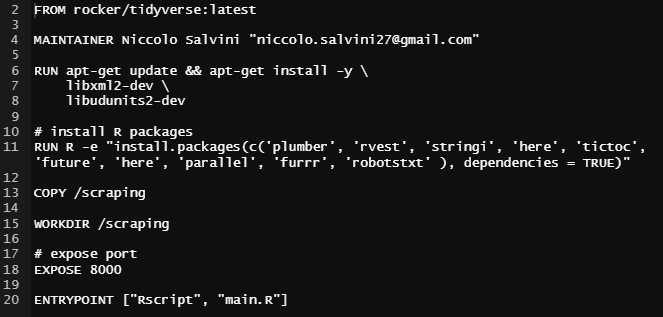
\includegraphics{images/dockerfile2.PNG.jpg}
\caption{\label{fig:dockerfile}Custom Dockerfile from salvini/api-immobiliare Docker Hub repository, author's source}
\end{figure}

Each line from the Dockerfile has its own specific role:

\begin{itemize}
\item
  \passthrough{\lstinline!FROM rocker/tidyverse:latest!} : The command imports from rocker project a pre set config guration containing the latest version of base-R along with the tidyverse \citep{tidyverse} R packages collection.
\item
  \passthrough{\lstinline!MAINTAINER Niccolo Salvini "niccolo.salvini27@gmail.com"!} : The command tags the maintainer and its e-mail contact information.
\item
  \passthrough{\lstinline!RUN apt-get update \&\& apt-get install -y \\ libxml2-dev \\ libudunits2-dev!} : The command update and install remaining ``lower'' Linux dependencies required to run Plumber and rvest.
\item
  \passthrough{\lstinline!RUN R -e "install.packages(c('tictoc','here','...',dependencies=TRUE)!} : The command install all the further lower level libraries required to execute the files. Since some packages have inner dependencies the option \passthrough{\lstinline!dependencies=TRUE!} is necessary.
\item
  \passthrough{\lstinline!COPY /scraping!} : The command tells Docker to copy into the container files in /scraping folder (where API specs are)
\item
  \passthrough{\lstinline!WORKDIR /scraping!} : The command tells Docker to set /scraping as working directory
\item
  \passthrough{\lstinline!EXPOSE 8000!} : The commands instructs Docker engine that the container listens on the specified network ports 8000 at runtime. Default \emph{transportation} layer is TCP.
\item
  \passthrough{\lstinline!ENTRYPOINT ["Rscript", "main.R"]!} : the command tells docker engine to execute the file main.R where are contained the Plumber router options (i.e.~host and port specifications).
\end{itemize}

\hypertarget{nginx}{%
\section{NGINX reverse Proxy Server and Authorization}\label{nginx}}

Proxy server in this context offers the opposite angle for the exact same security problem. As a matter of fact the downside is that they can be exploited for the same reason for which they have been criticized at the end of section (\ref{spoofing}). Reverse Proxy server are a special type of gateway \ref{def:proxy} that is usually located behind a private network firewall to route client requests to the corresponding backend server \citep{nginxDocs}. An reverse proxy offers an extra abstraction and control level to ensure that network traffic flows smoothly between clients and servers. NGINX as it can be inferred by its official documentation empowers traffic flows by:

\begin{itemize}
\item
  \emph{Load balancing}: A reverse proxy server will stand guard inf front of back end servers and redirect requests across a group of servers in a way that maximizes speed and capacity usage as well as not overloading the server. When a server crashes, the load balancer redirects traffic to the other online servers (note required since traffic is not expected to be enormous).
\item
  \emph{Web acceleration}: A reverse proxies can condense input and output data by caching frequently requested information. This assists traffic between clients and servers avoiding to request data more than once. They can also apply SSL encryption, which improves their performance by eliminating loads form web servers.
\item
  \emph{Security and anonymity}: A reverse proxy server protects identities and serves as an additional protection against security threats seen in sub-sections (\ref{sanitize}, \ref{Dos}) by intercepting requests before they reach end server.
\end{itemize}

When a user calls the API, NGINX acts as a gateway asking for credentials and registering log data (HTTP identification headers). If the request has already been asked then cached response is returned. If it does not then the request is routed to the endpoint, service A and B in figure \ref{fig:nginxfun}. Endpoints elaborate the request into the response, which flows back at first to the gateway and then finally to the client. Logging data can be feeded to a dashboard monitoring traffic and API exposure.

\begin{figure}
\centering
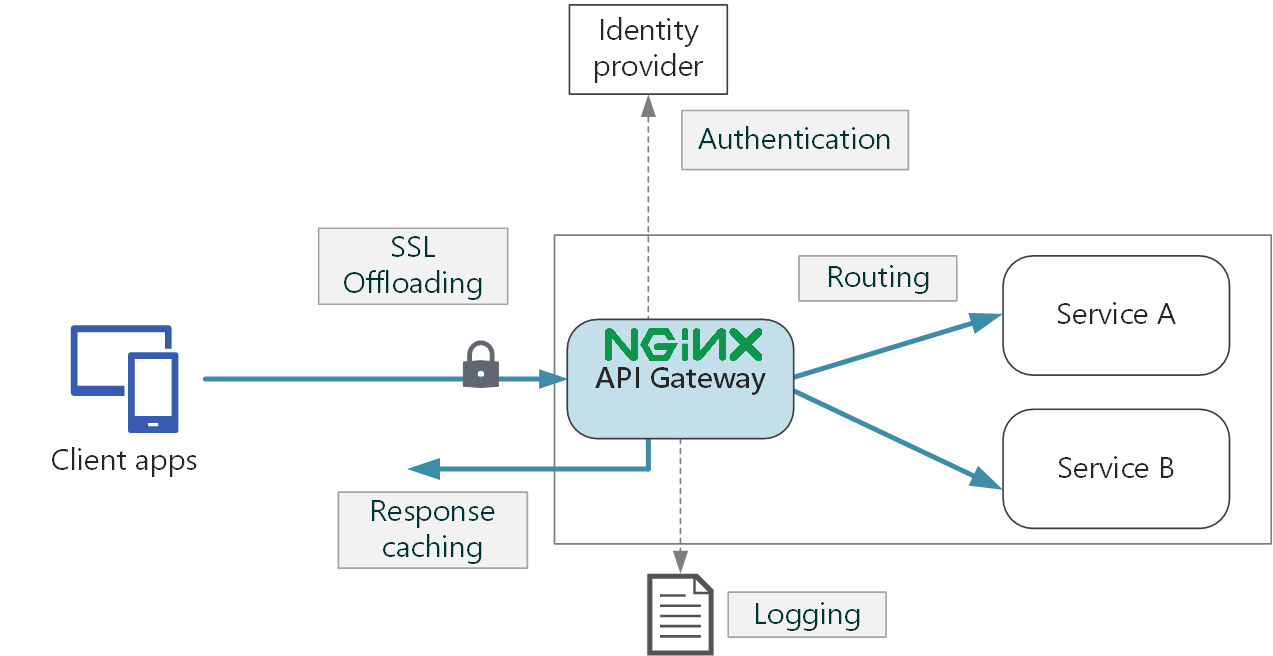
\includegraphics{images/nginx_gateway.png}
\caption{\label{fig:nginxfun}NGINX gateway redirecting an incoming request, source \citet{azureNGINX}}
\end{figure}

Then without any further software installation, the developer can simply make use of the latest NGINX open sourced image to build the NGINX proxy server within the same image. A further configuration file should manage NGINX inner settings that links volumes, ports and IPs, but details are beyond the scope of the analysis.

\hypertarget{docker-compose}{%
\section{Docker-Compose}\label{docker-compose}}

Compose is a multi-container Docker framework to define and run complex application and services, that means isolated stand alone containers can communicate one to each other. The orchestration of containers is managed through a .yaml file docker-compose.yml that configures the whole set of facilities designed for the services. Services are then build with a single docker command \passthrough{\lstinline!docker-compose up!} on the basis of the instruction yaml file. Compose also enables \emph{Volumes}, which are used in Docker for \textbf{data persistence} \citep{dockervolumes}. VOlumes allows to keep data secured from docker stop or delete containers. Docker Volumes ina nutshell works as the linkage between a physical file system path (folders, directories) plugged/\textbf{mounted} into the virtual container file system path.
The main properties for Composition as in documentation \citep{docker_documentation_2020} regards:

\begin{itemize}
\tightlist
\item
  \emph{A central host in multiple isolated environments}: Compose provides a label for a project to distinguish environments. The default project name is the directory path.
\item
  \emph{Preserve data volumes (which are the preferred Docker mechanism to consume data generated and used by containers) when building containers}: Compose maintains all of the services' Volumes. When Docker-compose is running, it transfers the Volumes from the old container into the new container when it detects containers from previous runs. This method guarantees that no Volume data produced is lost.
\item
  \emph{Only recreate containers that have changed}: Compose caches the configuration and re-use the same containers when it reboot a service which hasn't changed. Re-use containers means it provides really fast improvements to the environment when developing complex services.
\item
  \emph{Variables and moving a composition between environments}: Compose supports file variables which might be used to adjust any composition to various environments or users.
\end{itemize}

\begin{figure}
\centering
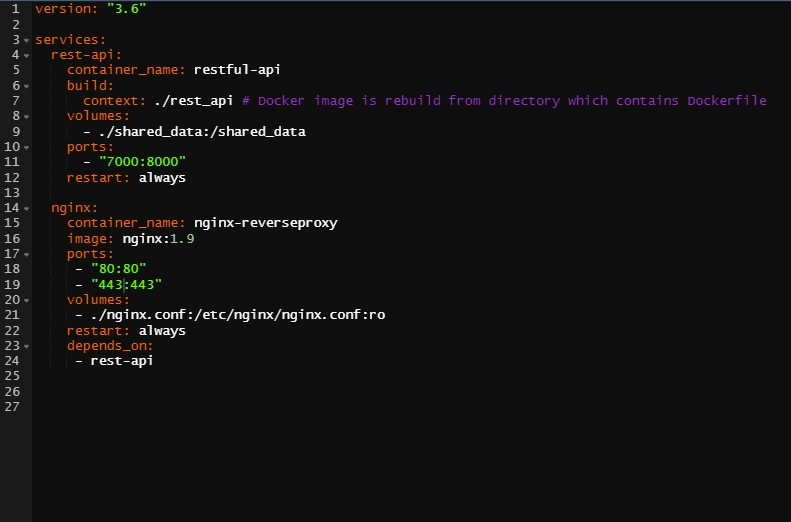
\includegraphics{images/docker-compose.jpg}
\caption{\label{fig:Compose}Docker Compose YAML file orchestration for NGINX container and RESTful API, author's source}
\end{figure}

The first line defines the versions according to which Compose orchestrates containers. Services are two, the rest-api and NGINX. The former whose name is restful-api builds the container starting from the Dockerfile contained into the rest\_api path specified as in \ref{dockerfile}. The first service also mounts Volumes from shared\_data to itself in the virtual container file path. Port 8000 opened (\ref{dockerfile}) is linked to the 7000 one. Restarting set to ``always'' secures the latest container version.
The latter service is NGINX \ref{nginx} which proxies traffic from 80 and 443 based on .conf file whose specifications are beyond the scope of the analysis. Volumes makes sure that specifications are arranged in the default path choice. The option depends\_on defines the chrono-logical condition accroding to which containers should be run and then composed.

\hypertarget{HTTPS}{%
\section{HTTPS(ecure) and SSL certificates}\label{HTTPS}}

Communication even though properly secured and distributed with NGINX is still not encrypted so sensitive data are still being exposed. HTTP Secured (HTTPS) is a product of HTTP combined with SSL/TLS (Secure Sockets Layer/Transportation Security Layer) protocol rather than a protocol itself. HTTPS is strictly appropriate when transmitting sensitive data such as banking or on-line buying. Its importance is highlighted by the fact that nowadays is rather more common to find HTTPS than HTTP. The Secured method encrypts all contacts between the client and the server, figure \ref{fig:httpsmeth}. The HTTPS scheme in actual is ``HTTPS'' and its default port is 443 (that should be exposed too in the dockerfile). SSL runs as a sublayer of the \emph{application} layer (a further internet layer, refer to section \ref{HTTPmethod}), this ensures that HTTP messages are encrypted prior being transmitted to the server (SSL Offloading box in figure \ref{fig:nginxfun}) whether it is a proxy server or directly a web server.

\begin{figure}
\centering
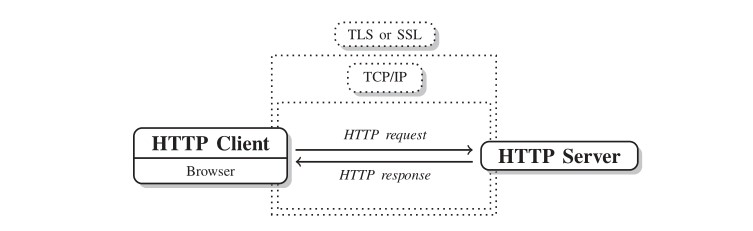
\includegraphics{images/https_method.jpg}
\caption{\label{fig:httpsmeth}HTTPS encryption with SSL certificates, source \citet{automateddatacollection}}
\end{figure}

From a port communication point of view at first NGINX container listens to on port 80 and that it is where all requests should relay to IP\_macchine\_address:8000. As a result the RESTful API is published on Port 80 instead of 8000. Secondly it listens on the SSL port 443 and points to the key and certificate files that have been created in the Dockerfile.

\hypertarget{aws}{%
\section{AWS EC2 instance}\label{aws}}

From henceforth the software container environment can be reproduced regardless of the mounted OS. Scalability and accessibility is worked out by exporting orchestrated containers on a web server. There are many hosting services options that varies primary on the budget and consequently on the API audience. A flexible cloud provider combined with NGINX load balancing \emph{ceteris paribus} may offer a stable and reliable service for a reasonable price, even considering a bad-case scenario where requests are many and insistent.
\begin{definition}[AWS EC2]
\protect\hypertarget{def:aws}{}{\label{def:aws} \iffalse (AWS EC2) \fi{} }Amazon Elastic Compute Cloud (EC2) is a web service that contributes to a secure, flexible computing capacity in the AWS cloud. EC2 allows to rent as many virtual servers as needed with customized capacity, security and storage.
\end{definition}

AWS EC2 represents a popular hosting option, most importantly this path is already narrowed by many open source contributors. The selected target is a AWS free tier t3.micro whose specifications are: 2 vCPU (Virtual CPU), 1 GB memory and a mounted Ubuntu distribution OS. Moreover T3 instances are known to provide device, memory, and network resource balance and have been developed for applications that experience transient spikes in use with modest CPU use. They are designed especially to serve low-latency interactive applications, small and medium databases, virtual desktops, development environments, code repositories, and business-critical applications, therefore they suit the needs.
Prior any new instance initialization AWS offers to tune servers' set up options. Networking and VPC are chosen to be left as is since they can always be updated at need. Storage is increased to 30 GB which represents the free tier eligibility upper limit. Tags are not required. Indeed security at first needs to account for a SSH connection that allows communication with the server i.e.~open port 22. Secondly it should account for port openings accordingly to NGINX configuration file and rest-api dockerfile (\ref{dockerfile}), port 80 (default for TCP) and 443 (HTTPS default) are opened. Once the instance is running the server can be accessed through SSH (Putty or Bash depending on the OS) behind authentication.

\hypertarget{sdwf}{%
\section{Software CI/CD Workflow}\label{sdwf}}

Software changes can happen quite often due to the dynamic nature of the RESTful API's target website. This requires a modern stack of cloud technologies to update, revert and quickly deoply software versions, or even adapt software architecture. As a consequence the software CI/CD manages minor changes with local commits to the project, which are then directly pushed through git into a GitHub repository, upper left quadrant \ref{fig:sfmap}. The repository directly communicates with an open DockerHub repository that sequentially triggers the compose-up command of the compose.yml file, and through that the docker images whenever any changes are pushed, upper right quadrant \ref{fig:sfmap}. Images are tagged and cached so that versions are controlled and Software build avoids to rerun containers that have not suffered any change. Debugging stage is constrained by logs generated by docker engine. Furthermore the build stage in R since 2019 required long time due to package compiling, but since the appearance of Rstudio \href{https://packagemanager.rstudio.com/client/\#/}{package manager} which includes beta support for pre-compiled R packages they can be installed 3 times faster \citep{nolispmanager}.
When newer images are available they can be pulled from the EC2 server and rerun in detached mode. Massive software changes are managed through GitHub branches, even though it must be kept in mind to swith lautomatic building brench. The Ec2 server is associated to an Elastic IPs address allowing to reuse the address for external databases connections and DNS services as Cloudflare (for SSL certificates). Moreover elastic IPs are effective when the EC2 server stands in need of upgrading or downgrading or when the server may fail, thus restoring and apply the IP address for a new server.

\begin{figure}
\centering
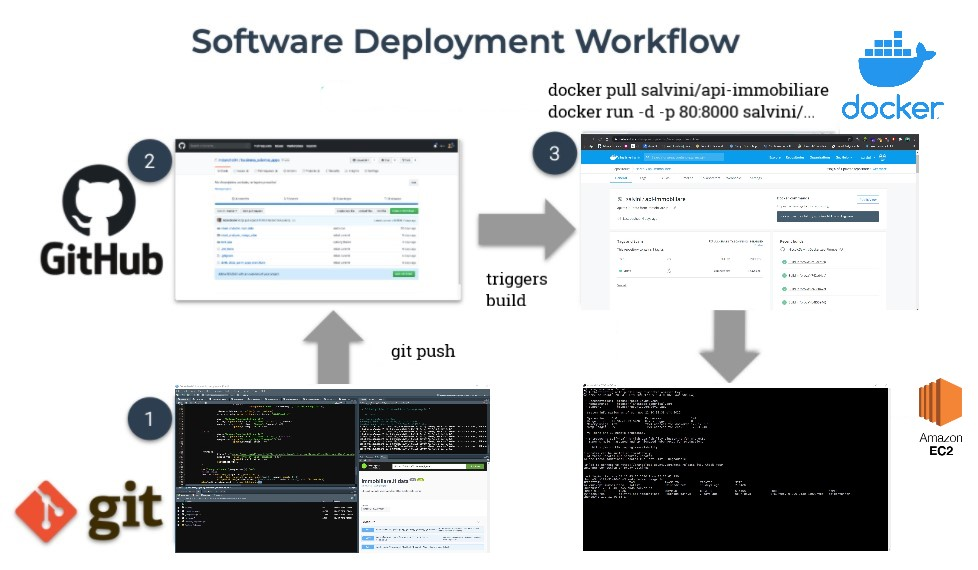
\includegraphics{images/SoftwareDevWF.jpg}
\caption{\label{fig:sfmap}Sofwtare development workflow, author's source}
\end{figure}

\hypertarget{further-sf-integrations}{%
\section{Further SF Integrations}\label{further-sf-integrations}}

A more robust code can be obtained embedding recent R software development frameworks as \passthrough{\lstinline!Golem!} \citet{colin_fay_2020} into the existing structure, anyway this will require a complete restyle of the existing code structure. The framework stimulates the usage of \emph{modules} to enhance reusable codes. In addition for the way it is done it forces through automatic actions, articulated into a sequence of steps, to organize code and dependencies aimed at saving time to DevOps teams. It has also a convenient function to build custom dockerfiles based on the dependecies stated throughout the building framework.
This is also truer according to the latest API literature which suggests (Shiny services as well) to wrap up code into R packages as in \citet{plungr}, Which wraps around the aforementioned concepts to the specific API Plumber \citet{plumber} framework. This is extensively treated in section 4.2 \citet{colin_fay_2020} and in the \href{https://deanattali.com/2015/04/21/r-package-shiny-app/}{comment} by Dean Attali, as a matter of fact Golem is built upon the idea of package portability. Thanks to packages \textbf{TDD} (i.e.Test-Driven Development \citet{TDD_2004}) through the library \citet{testthat} can make software more reliable, and production grade. Moreover Loadtest \citet{loadtest} can help figure out the traffic congestions visualizing sessions and enabling monitoring dashboards.
A popular API development integration service and automate testing tool \href{https://www.postman.com/}{Postman}, which does its best when POST requests endpoints are served, since for the moment they are not required it is not used.
Pins is an r packages \href{https://rstudio.com/resources/rstudioconf-2020/deploying-end-to-end-data-science-with-shiny-plumber-and-pins/?mkt_tok=eyJpIjoiTmprNU1USXhPVEprWXpNMSIsInQiOiJtTUhKVzlvSjVIV2hKc0NRNVU1NTRQYSsrRGd5MWMyemlTazQ5b1lHRGJXNVBLcnpScjZRaWVcL2JGUjBPNGIwV3pwY1dKTW45cnhcL2JzZUlGWndtSFNJZVNaOUcyc1ZXcEJOcnppSVJXSGZRSVU1ZUY1YUU2NWdDamoxZG5VMHZcLyJ9}{this link}
software development framework and tools for testing \href{https://github.com/isteves/plumbplumb}{this work}

\hypertarget{inla}{%
\chapter{INLA computation}\label{inla}}

Due to convergence issues and heavy calculations, Bayesian Inference - by MCMC \citep{mcmc} and MC techniques - may be a challenge in terms of computational burdens, this is also more critical for spatial and spatio-temporal model settings \citep{Cameletti2012}. The computational aspect refers in particular to the ineffectiveness of linear algebra operations with large dense covariance matrices which are common into the aforementioned settings.
INLA \citep{Rue2009} stands for Integrated Nested Laplace Approximation and constitutes a computational alternative to traditional Baeysian Inference estimation methods focused on a special type of gaussian spatial processes Gaussian Markov Random Field (GMRF) \citep{GMRFRue}. INLA zoom in models that can be expressed as Latent GMRF which are special types of spatial processes shaping spatial data dependence observed on areal units as regular grid, lattice or geospatial data.
This turns out to cause a computational gain reducing time of model fitting \citep{Bayesian_INLA_Rubio} since matrices in this context are very sparse. Furthermore, INLA approximates the posterior marginal distributions of the model parameters with Laplace approximation which results in a considerably high accuracy.
Other benefits of using INLA algorithm are capitalized by Rue in \citep{YT:Rue}:

\begin{itemize}
\tightlist
\item
  Can define very complex/nested parameters models within that framework.
\item
  Most important statistical models are actually LGM.
\item
  Very good support for spatial models.
\item
  Extension to spatio-temporal model
\end{itemize}

The chronological steps followed in the arguments presentation retraces the one from Blangiardo and Cameletti \citep{Blangiardo-Cameletti} and Rubio \citep{Bayesian_INLA_Rubio}, which is also the default option for all the main authorities in the field. The choice is also to overlook mathematical dense details and directly jump on the statistical intuition and the practical application of the algorithm.

In the end it is presented the R-INLA project and the package which are found in last section focusing on the core functions and main arguments.
Notation is inherited by \citet{Blangiardo-Cameletti} because it is more straightforward, neverthelesss it differs from the original paper by Rue, Chopin and Martino \citeyearpar{Rue2009}. As further remarks, bold symbols are intended as vectors, so each time they occur they have to be considered like the \emph{ensamble} of their values. The notation \(\pi(\cdot)\) is a generic notation for the density of its arguments.

\hypertarget{LGM}{%
\section{The class of Latent Gaussian Models LGM}\label{LGM}}

Given some observations \(y_{i \ldots n}\), the goal is to set up a Latent Gaussian Model LGM. As a first step it is convenient (even though not strictly necessary as in \citeyearpar{Bayesian_INLA_Rubio}) to specify an \emph{exponential family} distribution function characterized by some parameters \(\phi_{i}\) (usually expressed by the mean \(\left.E\left(y_{i}\right)\right)\)) and other hyper-parameters \(\psi_{k} ,\forall k \in \ 1\ldots K\). . Furthermore, these observations will have an associated likelihood \citeyearpar{Bayesian_INLA_Rubio}. The parameter \(\phi_{i}\) can be defined as an additive \emph{latent linear predictor} \(\eta_{i}\), as in Krainski and Rubio (\citeyearpar{Krainski-Rubio}), through a \emph{link function} \(g(\cdot)\), i.e.~\(g\left(\phi_{i}\right)=\eta_{i}\). A comprehensive expression of the linear predictor takes into account all the possible effects on covariates:

\[
\eta_{i}=\beta_{0}+\sum_{m=1}^{M} \beta_{m} x_{m i}+\sum_{l=1}^{L} f_{l}\left(z_{l i}\right)
\]

where \(\beta_{0}\) is the intercept, \(\boldsymbol{\beta}=\left\{\beta_{1}, \ldots, \beta_{M}\right\}\) are the coefficients that quantifies the linear effects of covariates \(\boldsymbol{x}=\left({x}_{1}, \ldots, {x}_{M}\right)\) and \(f_{l}(\cdot), \forall l \in 1 \ldots L\) are a set of random effects defined in terms of a \(\boldsymbol{z}\) set of covariates \(\boldsymbol{z}=\left(z_{1}, \ldots, z_{L}\right)\) (e.g.~rw, ar1) \citep{Blangiardo-Cameletti}. As a consequence of the extended possibilities of combining mixed effects into LGMs, they contain a wide range of models e.g.~GLM, GAM, GLMM, linear models and spatio-temporal models. This constitutes one of the main advantages of INLA algorithm, since it can fit many different models and integrate older ones with newer parameters. Furthermore INLA contributors recently are extending the methodology to many different areas of application and integrating the LG class with many other random effects \emph{miss lit Martins et al., 2013 }.
With that said all the latent field components can be grouped into a variable denoted with \(\boldsymbol{\theta}\) such that: \(\boldsymbol{\theta}=\left\{\beta_{0}, \boldsymbol{\beta}, f\right\}\) whose distribution depends on the hyper-paramenter \(\boldsymbol{\psi}\). The analogue can be repeated for hyper-parameters obtaining \(\boldsymbol{\psi} = \left\{\psi_{1}, \ldots, \psi_{K}\right\}\).
Then the probability distribution function conditioned to both parameters and hyper parameters is:

\[
y_{i} \mid \boldsymbol{\theta}, \boldsymbol{\psi} \sim \pi\left(y_{i} \mid \boldsymbol{\theta},\boldsymbol{\psi}\right)
\]

Since data \(\left(y_{1}, \ldots, y_{n}\right)\) is drawn by the same distribution family but it is also conditioned to parameters which are said \emph{conditional independent} \citep{GMRFRue} (i.e.~\(\pi\left(\theta_{i}, \theta_{j} \mid \theta_{-i, j}\right)=\pi\left(\theta_{i} \mid \theta_{-i, j}\right) \pi\left(\theta_{j} \mid \theta_{-i, j}\right)\)) , then the joint distribution is given by the product of all the independent parameters i.e.~the likelihood. Note that the product index \(i\) ranges from 1 to \(n\), i.e.~\(\mathbf{I} = \left\{1 \ldots n \right\}\).
In the case when an observation is missing, i.e.~\(i \notin \mathbf{I}\), INLA automatically discards missing values from the model estimation \citeyearpar{Bayesian_INLA_Rubio}, this would be critical during missing values imputation \ref{missassimp}.
The likelihood expression is, where \(\boldsymbol\theta^{\prime}\) is the transposed version of \(\boldsymbol\theta\) and the \(|\cdot|\) is the determinant:

\begin{equation}
\pi(\boldsymbol{y} \mid \boldsymbol{\theta}, \boldsymbol{\psi})=\prod_{i \in \mathbb{I}} \pi\left(y_{i} \mid \theta^{\prime}_{i}, \boldsymbol{\psi}\right)
\label{eq:likelihood}
\end{equation}

Each data point is connected to a single combination \(\theta_{i}\) in the \(\boldsymbol{\theta}\) \emph{latent field}. In fact the latent aspect of the field regards the undergoing existence of many parameter combination. Furthermore hyper-parameters are by definition independent, in other words \(\boldsymbol{\psi}\) is the product of many univariate priors \citep{Bayesian_INLA_Rubio}. A Multivariate Normal distribution prior is imposed on the latent field \(\boldsymbol{\theta}\) such that it is centered in 0 with precision matrix \(\boldsymbol{Q(\psi)}\) (the inverse of the covariance matrix \(\boldsymbol{Q}^{-1}(\boldsymbol{\psi})\)) depending only on \(\boldsymbol{\psi}\) hyper-parameter vector i.e., \(\boldsymbol{\theta} \sim \operatorname{Normal}\left(\mathbf{0}, \boldsymbol{Q}^{-1}(\boldsymbol{\psi})\right)\). As a notation remark some authors choose to keep the covariance matrix expression as \(\boldsymbol{Q}\) and its inverse precision matrix as \(\boldsymbol{Q}^{-1}\), equation \eqref{eq:gmrf}. Using the covariance instead of precision is strongly not encouraged essentially for two reasons: the first is a practical one and regards the default hyper-paramater argument option in R INLA library, which adopts precision matrix notation. While the second accounts \citep{GMRFRue} the relationship between conditional independence and the
zero structure of the precision matrix, left in figure \ref{fig:precvscov}, that is dense in the covariance matrix, right in figure \ref{fig:precvscov} notation case.

\begin{figure}
\centering
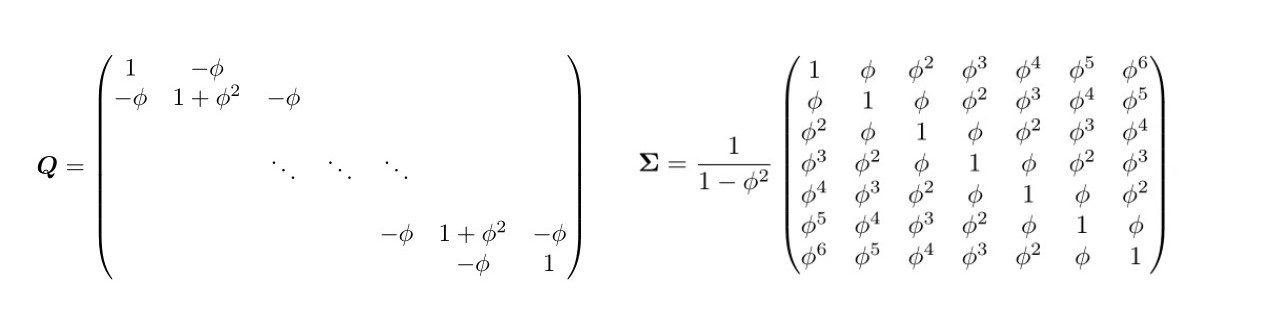
\includegraphics{images/precvscov.jpg}
\caption{\label{fig:precvscov}Precision Matrix in GMRF vs the Covariance matrix, source \citet{GMRFRue}}
\end{figure}

The exponential family density function can be rewritten as:

\begin{equation}
\pi(\boldsymbol{\theta} \mid \boldsymbol{\psi})=(2 \pi)^{-n / 2}| \boldsymbol{Q(\psi)}|^{1 / 2} \exp \left(-\frac{1}{2} \boldsymbol{\theta} \boldsymbol{Q(\psi)} \boldsymbol{\theta}\right)
\label{eq:gmrf}
\end{equation}

The conditional independence assumption on each \(\theta_i\) element of the latent field \(\boldsymbol{\theta}\) leads \(\boldsymbol{Q^{-1}(\psi)}\) to be a sparse precision matrix since for a general pair of combinations \(\theta_{i}\) and \(\theta_{j}\), when \$ i \neq j\$, the resulting element in the precision matrix is 0 i.e.~\(\theta_{i} \perp \theta_{j} \mid \theta_{-i, j} \Longleftrightarrow Q_{i j}(\boldsymbol{\psi})=0\) \citeyearpar{Blangiardo-Cameletti}, where the notation \(x_{-i}\) denotes all elements in \(\boldsymbol{x}\) but \(x_{-i}\).
A probability distribution whose characteristics are the aforementioned is named \emph{Gaussian Markov random field} (\textbf{GMRF}). GMRF as a matter of fact are Gaussian Variables with \emph{Markov properties} encoded in the precision matrix \(\boldsymbol{Q}\) \citep{Rue2009}. The computational gain of doing inference with a GMRF is directly related to the sparse precision matrix \(\boldsymbol{Q}\) structure. In fact, it can be done using numerical methods for the sparse matrices in linear algebras, leading to a substantial computational benefit \citep{Cameletti2012}, \citep{GMRFRue}, for the specific algorithms.
Once priors distributions are specified both for\(\boldsymbol{\theta}\) and \(\boldsymbol{\psi}\), then the joint posterior distribution is obtained by the product of the \emph{GMRF} \eqref{eq:gmrf} density, the \emph{likelihood} \eqref{eq:likelihood} and the hyper-parameter prior distribution:

\[
\pi(\boldsymbol{\theta}, \boldsymbol{\psi} \mid y)\propto  \underbrace{\pi(\boldsymbol{\psi})}_{\text {prior }} \times \underbrace{\pi(\theta \mid \psi)}_{\text {GMRF }} \times \underbrace{\prod_{i=1}^{n} \pi\left(y_{i} \mid \theta_{i}, \boldsymbol{\psi}\right)}_{\text {likelihood }}
\]
Which can be further rewritten as in \citep{Blangiardo-Cameletti} as:

\[
\begin{aligned}
\pi(\boldsymbol{\theta}, \boldsymbol{\psi} \mid y) & \propto \pi(\boldsymbol{\psi}) \times \pi(\boldsymbol{\theta} \mid \boldsymbol{\psi}) \times \pi(y \mid \boldsymbol{\theta}, \boldsymbol{\psi}) \\
& \propto \pi(\boldsymbol{\psi}) \times \pi(\boldsymbol{\theta} \mid \boldsymbol{\psi}) \times \prod_{i=1}^{n} \pi\left(y_{i} \mid \theta_{i}, \boldsymbol{\psi}\right) \\
& \propto \pi(\boldsymbol{\psi}) \times|\boldsymbol{Q}(\boldsymbol{\psi})|^{1 / 2} \exp \left(-\frac{1}{2} \boldsymbol{\theta}^{\prime} \boldsymbol{Q}(\boldsymbol{\psi}) \boldsymbol{\theta}\right) \times \prod_{i}^{n} \exp \left(\log \left(\pi\left(y_{i} \mid \theta_{i}, \boldsymbol{\psi}\right)\right)\right)
\end{aligned}
\]

In the end joining exponents by their multiplicative property

\begin{equation}
\pi(\boldsymbol{\theta}, \boldsymbol{\psi} \mid y) \propto \pi(\psi) \times|\boldsymbol{Q}(\boldsymbol{\psi})|^{1 / 2} \exp \left(-\frac{1}{2} \boldsymbol{\theta}^{\prime} \boldsymbol{Q}(\boldsymbol{\psi}) \boldsymbol{\theta}+\sum^{n} \log \left(\pi\left(y_{i} \mid \theta_{i}, \boldsymbol{\psi}\right)\right)\right)
\label{eq:jointpostdistr}
\end{equation}

\hypertarget{approx}{%
\section{INLA Approximate Inference setting}\label{approx}}

INLA is not going to try to estimate the whole joint posterior distribution from expression \eqref{eq:jointpostdistr}. Instead it will try to estimate the posterior marginal distribution for each \(\theta_{i}\) combination in the latent parameter \(\boldsymbol{\theta}\), given the hyper parameter priors specification \(\psi_{k}\). Proper estimation methodsa through Laplace Approximation however are beyond the scope of the analysis, further excellent references focused on the task are Rubio \citeyearpar{Bayesian_INLA_Rubio} in section 2.2.2 and Blangiardo \& Cameletti \citeyearpar{Blangiardo-Cameletti} in section 4.7.2.
The final goal of Bayesian Inference is to compute marginal posterior distribution function for each latent parameter element \(\theta_{i}\) in \(\boldsymbol\theta\)

\begin{equation}
  \pi(\theta_{i} \mid \boldsymbol{y})=\int \pi(\boldsymbol{\theta}, \boldsymbol{\psi} \mid \mathbf{y}) \pi(\boldsymbol{\psi} \mid \mathbf{y}) d \psi
\label{eq:latentparam}
\end{equation}

As well as the marginal posterior distribution for each hyper-parameter \(\psi_{k} \in \boldsymbol\psi\),

\begin{equation}
  \pi\left(\psi_{k} \mid y\right)=\int \pi(\boldsymbol{\psi} \mid y) d \psi_{-k}
  \label{eq:hyperparam}
\end{equation}

Both of the integrals in \eqref{eq:hyperparam} and \eqref{eq:latentparam} are integrated over the \(\boldsymbol\psi\), as a result am approximation of the joint posterior distribution is desired \citep{Krainski2018}. Following the notation by Rue \citeyearpar{Rue2009} the integral approximations for hyper-parameters are \(\tilde\pi\left(\boldsymbol{\psi} \mid \boldsymbol{y}\right)\) and are plugged in \eqref{eq:latentparam} to obtain the approximation for the posterior marginal of the latent parameter.

\[
\tilde{\pi}\left(\theta_{i} \mid y\right) \approx \sum_{j} \tilde{\pi}\left(\theta_{i} \mid \boldsymbol{\psi}^{(j)}, y\right) \tilde{\pi}\left(\boldsymbol{\psi}^{(j)} \mid y\right) \Delta_{j}
\]
where \(\Delta_{j}\) are the weights associated with a set of \(\psi_{k}\) in a grid \citep{Krainski2018}. The estimate of \(\tilde\pi\left(\boldsymbol{\psi} \mid \boldsymbol{y}\right)\) can be determined in various ways. In order to minimize numerical error \citet{Rue2009} also addresses how this approximation should be.

\hypertarget{inlahier}{%
\section{INLA as a Hierarchical Model}\label{inlahier}}

INLA setting presented in section \ref{approx} can be reorganized following a \emph{Hierarchical structure} which allows to handle different level parameters in a more compact and coherent way.
Since each of the element of the latent field \(\boldsymbol{\theta}\) defined in section \ref{LGM}, which groups all the latent components, is assumed to be similar to each of the other. And since each element comes from a distribution \(\pi\left(\theta_{j} \mid \psi\right)\) sampled with the same hyper parameters, \(\boldsymbol \psi\). Then there are at least two different levels of the analysis. One lower that regards the \(\theta_j\) depending on the one higher the \(\boldsymbol\psi\).
The fact that \(\theta_j\) are generated by the same distribution authorizes each \(\theta_j\) and \(\theta_i\) (\(i \neq j\)) to \emph{exchange} information, which it is totally different from model settings seen before since they were totally independent. As an example under the frequentist assumption of iid samples the joint prior distribution for \(\boldsymbol\theta\) can be rewritten in terms of the product of the each marginal distributions, i.e \emph{likelihood}:

\[
\pi\left(\theta_{1}, \ldots, \theta_{J}\right)=\prod_{j=1}^{J} \pi\left(\theta_{j}\right)=\pi(\theta)^{J}
\]
Indeed when a hierarchical structure is imposed on the parameters \(\boldsymbol\theta\) each single one is said \emph{Exchangeable} to the other with respect to the same random generating process. All the \(\theta_j\) share the same distribution characterized by the hyper-parameters \(\boldsymbol\psi\).

\begin{equation}
  \pi\left(\theta_{1}, \ldots, \theta_{J} \mid \psi\right)=\int \prod_{j=1}^{J} \pi\left(\theta_{j} \mid \psi\right) \pi(\psi) \mathrm{d} \psi
\label{eq:exchange}
\end{equation}

One of the major benefits of expressing hierarchy through integral in \eqref{eq:exchange} is the fact that levels can be extended to more than, say 3 (spatio-temporal models \citep{PACI2017149}).
Then when a Hierarchical structure is imposed on INLA at first, following \ref{LGM}, it is required to specify a probability distribution for \(\boldsymbol{y} = \left(y\left(s_{1}\right), \ldots, y\left(s_{n}\right)\right)=\left(y_{1}, \ldots, y_{n}\right)\). A Gaussian distribution for simplicity is chosen.

As a \emph{first level} parameters are picked up an \textbf{exponential family} sampling distribution (i.e.~Normally distributed, Gamma one other choice), which is \emph{exchangeable} with respect to the \(\boldsymbol{\theta}=\left\{\beta_{0}, \boldsymbol{\beta}, f\right\}\) \emph{latent field} and hyper parameters \(\boldsymbol{\psi_{1}}\), which includes also the ones coming from the latent Matérn GP process \(w_{i}\). The Spatial Guassian Process is centered in 0 and with Matérn covariance function as \(\tau^2\). \(w_{i}\) addresses the spatial autocorrelation between observation through a Matérn covariance function \(\mathcal{C}(\cdot | \boldsymbol\psi_{1})\) which in turn is tuned by hyper param included in \(\boldsymbol{\psi_1}\). Moreover the \(w_{i}\) surface has to be passed in the formula method definition \ref{example} via the \passthrough{\lstinline!f()!} function, so that INLA takes into cosideration the spatial component.

\[
\boldsymbol{y} \mid \boldsymbol{\theta}, \boldsymbol{\psi}_{1} \sim \mathrm{N}\left(\beta_{0}+ (\mathbf{X}_{i})^{\prime}\boldsymbol{\beta} + w_{i} ,  \tau^2 I_{n}\right)=\prod_{i=1}^{n} \mathrm{N}\left(y_{i} \mid \theta_{i}, \psi_{1}\right)
\]

Then at the \emph{second level} the latent field \(\boldsymbol{\theta}\) is characterized by a Normal distribution given the remaining hyper parameters \(\boldsymbol{\psi}_2\), recall the covariance matrix \(\boldsymbol{Q}^{-1}(\boldsymbol{\psi_{2}})\), depending on \(\boldsymbol{\psi_{2}}\) hyperparameters, is handled now by a Matérn covariace function depeding on its hyperparamter. This is done in order to map the GP spatial surface into a GMRF by SPDE solutions.

\[
\boldsymbol{\theta} \mid \boldsymbol{\psi}_{2} \sim \mathrm{N}\left(\boldsymbol{0}, \mathcal{C}( \cdot , \cdot  \mid \boldsymbol{\psi}_{2})\right)
\]

In the end hyper parameters \(\boldsymbol{\psi}=\left\{\boldsymbol{\psi_{1}}, \boldsymbol{\psi}_{2}\right\}\) having some specified prior distribution i.e.~\(\boldsymbol{\psi} \sim \pi(\boldsymbol{\psi})\),

\hypertarget{rinla}{%
\section{R-INLA package in Bayesian Regression}\label{rinla}}

INLA library and algoririthm is developed by the R-INLA project whose package is available on their website at their \href{http://www.r-inla.org}{source} repository. Users can also enjoy on INLA website a forum where daily discussion group are opened and an active community is keen to answer. Moreover It also contains a number of reference books, among which some of them are fully open sourced.
The core function of the package is \passthrough{\lstinline!inla()!}and it works as many other regression functions like \passthrough{\lstinline!glm()!}, \passthrough{\lstinline!lm()!} or \passthrough{\lstinline!gam()!}. Inla function takes as arguments the formula (where are response and linear predictor), the data (expects a data.frame obj) on which estimation is desired together with the distribution of the data. Many other methods inside the function can be added through lists, such as \passthrough{\lstinline!control.family!} and \passthrough{\lstinline!control.fixed!} which let the analyst specifying priors distribution both for \(\boldsymbol{\theta}\) parameters, \(\boldsymbol{\psi}\) hyper parameters and the outcome precision \(\tau\), default values are non-informative.
\passthrough{\lstinline!control.fixed!} as said regulates prior specification through a plain list when there only a single fixed effect, instead it does it with nested lists when fixed effects are greater than 2, a guided example might better display the behaviour:
\passthrough{\lstinline!control.fixed = list(mean = list(a = 1, b = 2, default = 0))!}
In the chuck above it is assigned prior mean equal to 1 for fixed effect ``a'' and equal 2 for ``b''; the rest of the prior means are set equal to 0.
Inla objects are inla.dataframe summary-type lists containing the results from model fitting. Objects contained in the \passthrough{\lstinline!inla()!} output function are summarized in \ref{fig:summartable}. Following Krainski \& Rubio \citeyearpar{Krainski-Rubio} data \(y(s_{1}), \ldots, y(s_{n})\) a taken from a generated toydataset and a hierarchical bayesian linear regression is fitted.

\begin{figure}
\centering
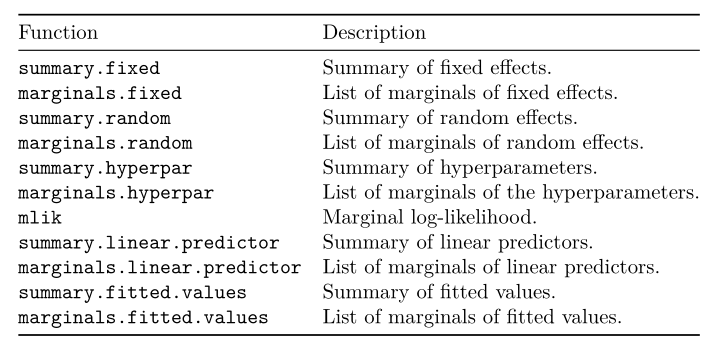
\includegraphics{images/summarytable.PNG}
\caption{\label{fig:summartable}summary table list object, source: \citet{Krainski-Rubio}}
\end{figure}

SPDEtoy dataset, that has a spatial component, and is generated from a \(y_{i}\) Gaussian variable; its moments are \(\mu_{i}\) and precision \(\tau\).

\begin{figure}
\centering
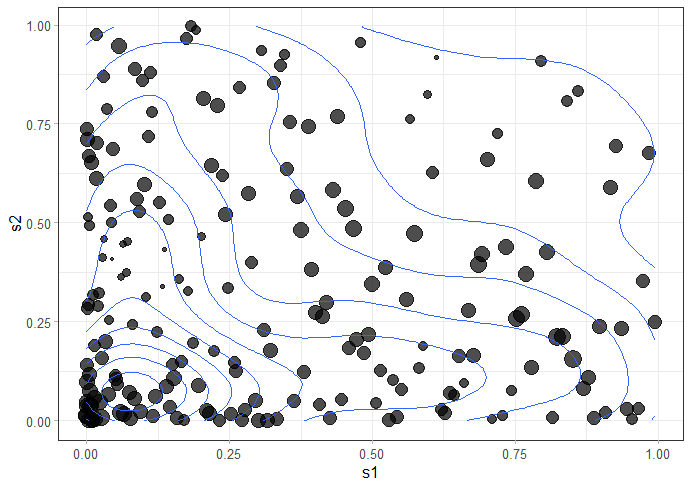
\includegraphics{images/cotour_toy.png}
\caption{\label{fig:SPDEplot}SPDEtoy plot, author's source}
\end{figure}

The mean moment in the Gaussian distribution \(\mu_{i}\) is expressed as the \emph{linear predictor} \(\eta_{i}\) (i.e.~\(E\left(y_{i} \mid \beta_{0}, \ldots, \beta_{M}, x_{i 1}, \ldots, x_{i M}\right) = \eta_{i}\) ). The function that maps the linear predictor into the parameter space is identity i.e.~\(\eta_{i}=\beta_{0}+\sum_{m=1}^{M} \beta_{m} x_{m i}+\sum_{l=1}^{L} f_{l}\left(z_{l i}\right)\).
After including in the model formula \(s_{1}\) and \(s_{2}\) spatial coordintates the linear predictor takes the following form: \(\eta_{i}=\beta_{0}+\beta_{1} s_{1 i}+\beta_{2} s_{2 i}\), where once again \(\beta_{0}\) is the fixed effect i.e.~intercept and the \(\beta_{j}\) are the linear effect on covariates. INLA allows also to include non-linear effects with the \passthrough{\lstinline!f()!} method inside the formula. \passthrough{\lstinline!f!} are pivotal in the follwing chpater \ref{prdm} since it incorporates the spatial component in the model through the Matérn covariance function,\ref{Matern}
As the last step prior distributions has to be chosen. The intercept prior is a uniform. Indeed Priors for Gaussian latent parameters are chosen to be vagues and they are set as 0 mean and 0.001 precision. In the end prior for the precision \(\tau\) is Gamma with parameters 1 and 0.00005. Models are sensitive to prior choices, as a consequence they are later revised at need.

The summary of the model specifications are:

\[
\begin{aligned}
y_{i} & \sim N\left(\mu_{i}, \tau^{-1}\right), i=1, \ldots, 200 \\
\mu_{i} &=\beta_{0}+\beta_{1} s_{1 i}+\beta_{2} s_{2 i} \\
\beta_{0} & \sim \text { Uniform } \\
\beta_{j} & \sim N\left(0,0.001^{-1}\right), j=1,2 \\
\tau & \sim G a(1,0.00005)
\end{aligned}
\]

\begin{lstlisting}[language=R]
data("SPDEtoy")
formula = y ~ s1 + s2
m0 = inla(formula, data = SPDEtoy)
\end{lstlisting}

\begin{tabular}{lrrrrrrr}
\toprule
  & mean & sd & 0.025quant & 0.5quant & 0.975quant & mode & kld\\
\midrule
(Intercept) & 10.1321487 & 0.2422118 & 9.6561033 & 10.1321422 & 10.6077866 & 10.1321497 & 7e-07\\
s1 & 0.7624296 & 0.4293757 & -0.0814701 & 0.7624179 & 1.6056053 & 0.7624315 & 7e-07\\
s2 & -1.5836768 & 0.4293757 & -2.4275704 & -1.5836906 & -0.7404955 & -1.5836811 & 7e-07\\
\bottomrule
\end{tabular}

The table in @ref(tab:table\_INLA) offers summary of the posterior marginal values for intercept and covariates' coefficients, as well as precision. Marginals distributions both for parameters and hyper-parameters can be conveniently plotted as in figure \ref{fig:marginalsplot}. From the table it can also be seen that the mean for s2 is negative, so the more is the value of the y-coordinate, the more the response decreases. That is factual looking at the SPDEtoy cotour plot in figure\ref{fig:SPDEplot}.

\begin{figure}
\centering
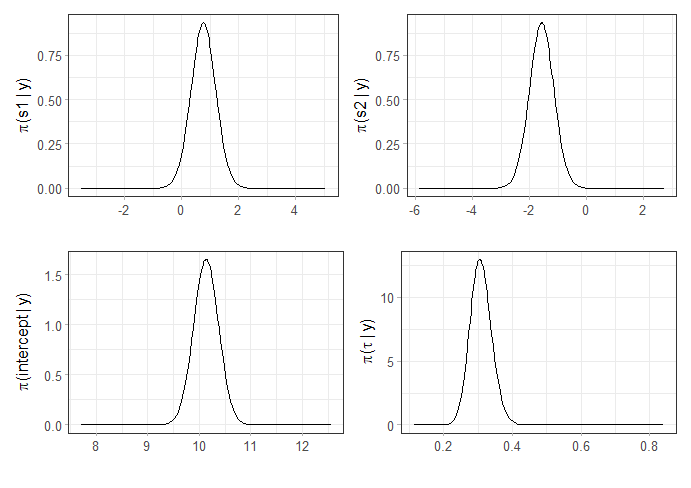
\includegraphics{images/marginal_distr.png}
\caption{\label{fig:marginalsplot}Linear predictor marginals, plot recoded in \passthrough{\lstinline!ggplot2!}, author's source}
\end{figure}

R-INLA enables also r-base style function to compute statistics on marginal posterior distributions for the density, distribution as well as the quantile function respectively with \passthrough{\lstinline!inla.dmarginal!}, \passthrough{\lstinline!inla.pmarginal!} and \passthrough{\lstinline!inla.qmarginal!}. One option which, packed into a dedicated function, computes the higher posterior density credibility interval \passthrough{\lstinline!inla.hpdmarginal!} for a given covariate's coefficient, such that \(\int_{q_{1}}^{q_{2}} \tilde{\pi}\left(\beta_{2} \mid \boldsymbol{y}\right) \mathrm{d} \beta_{2}=0.90\) with .1 Confidence Level, whose result is in table @ref(tab:higer\_posterior).

\begin{tabular}{lrr}
\toprule
  & low & high\\
\midrule
level:0.9 & -2.291268 & -0.879445\\
\bottomrule
\end{tabular}

Note that the interpretation is different from the traditional frequentist approach: in Bayesian statistics \(\beta_{j}\) comes from probability distribution, while frequenstists considers \(\beta_{j}\) as fixed unknown quantity whose estimator (random variable conditioned to data) is used to infer the value \citeyearpar{Blangiardo-Cameletti}.

\hypertarget{prdm}{%
\chapter{Point Referenced Data Modeling}\label{prdm}}

Geostatistical data are a collection of samples of geo type data indexed by coordinate Reference Systems (CRS), projected (e.g.~Eastings and Northings) or unprojected (e.g.~Latitude and Longitude), that originates from a spatially continuous phenomenon \citep{Moraga2019}. Data as such can monitor a vast range of phenomena, e.g.~disease cancer detection \citep{Bell2006} at several sites, COVID19 spread in China \citep{Li_Li_Ding_Hu_Chen_Wang_Peng_Shen_2020}, PM pollution concentration in a North-Italian region Piemonte \citep{Cameletti2012}. Moreover house prices variation, as observed in \citet{Bayesian_INLA_Rubio}, where house prices smoothly vary between closer neighborhoods. All the Examples taken before might document a spatial nature of data according to which closer observations can display similar values, this phenomenon is named spatial autocorrelation. Spatial autocorrelation conceptually stems from geographer Waldo Tobler whose famous quote, known as first law of geography, inspires geostatisticians:

\begin{quote}
``Everything is related to everything else,
but near things are more related than distant things''

\hfill --- Waldo R. Tobler
\end{quote}

Spatial models are explicitly designed to take into account this behavior and can separate spatial patterns from simply random spatial variance.
Spatial data can be partitioned into three spatial data type whose modeling tools are specific to their respective category.

\begin{itemize}
\tightlist
\item
  Areal Data
\item
  \textbf{Point Referenced Data}
\item
  Point Pattern Data
\end{itemize}

\begin{figure}
\centering
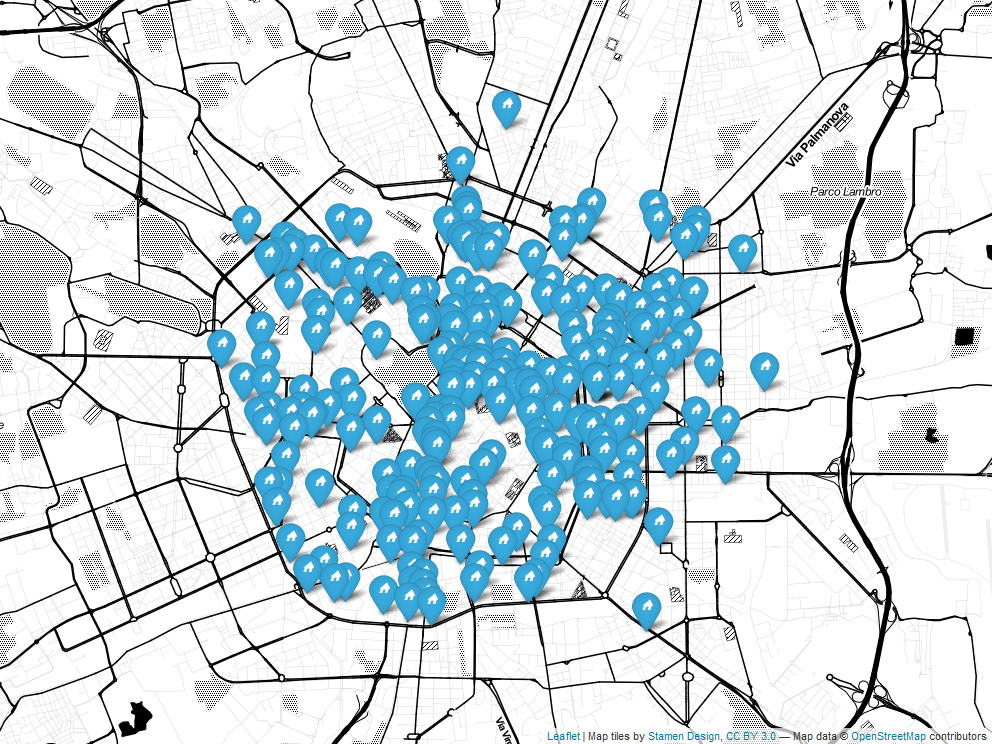
\includegraphics{images/map.png}
\caption{\label{fig:prdmap}Point Referenced Data map plot (\passthrough{\lstinline!Leaflet!} \citet{leaflet}) of a RESTful API call on Milan Rental Real Estate 20-11-2019, Author's Source}
\end{figure}

RESTful scraping API designed in chapter \ref{Infrastructure} extracts point referenced covariates in the form of Latitude and Longitude nested in a hidden source code JSON object. Observations are then plotted in figure \ref{fig:prdmap} obtaining a scattered map of houses with their respective geo-coordinates. Modeling methodologies described in this analysis will exclusively take into account point referenced techniques.
Then in order to extend data from discrete measurements (i.e.~point referenced) to a continuous spatial surface a stochastic process, namely Gaussian Process, has to be introduced and constrained to Stationarity and Isotropy. GP is then evaluated with a convenient covariance function, i.e.~Matèrn. The reason why Matérn is selected as candidate for covariance function relies in its flexibility and the fact that GP represented with Matérn covariance are able to determine a GMRF \ref{LGM} through the Stochastic Partial Differential Equations (SPDE) approach \citep{Cameletti2012}. The main benefit proceeding from a GF to a GMRF arises from the good computational properties that the latter appreciate.
Hedonic Price Models brings to the present analysis the theoretical foundation according to which covariates are added to the model.
Spatial kriging is essential to predict the process at new locations given the continuous spatial surface.
In the end models have to be checked and verified with resampling schemes which are once again specific to the data type and the scope of the analysis.

\hypertarget{GP}{%
\section{Gaussian Process (GP)}\label{GP}}

Point referenced data are defined as realizations of a stochastic process indexed by space.

\[
Y(s) \equiv\{y(s), s \in \mathscr{D}\}
\]
where \(\mathscr{D}\) is a (fixed) subset of \(\mathbb{R}^{d}\) (in the present work \emph{Latitude} and \emph{Longitude}, i.e.~\(d=2\)). The actual data can be then represented by a collection of observations \(\boldsymbol{y}=\left\{y\left(s_{1}\right), \ldots, y\left(s_{n}\right)\right\}\) (recall INLA notation in section \ref{LGM}) where the set \(\left(s_{1}, \ldots, s_{n}\right)\) points to the spatial location where data has been considered. For example, as in \citet{Cameletti2012}, assume to have collection of samples from air pollutant measurements obtained by observing a set of monitoring stations. Then The stochastic process \(Y(s)\) is observed in a fixed set of spatial indexes corresponding to the station locations (upwords arrows left in figure \ref{fig:prdproc}). This information is essential to interpolate points and build a spatially continuous surface (right panel in figure \ref{fig:prdproc}) over the y-studied variable domain in order to predict the phenomenon at locations not yet observed. \citep{LecturePaci}.

\begin{figure}
\centering
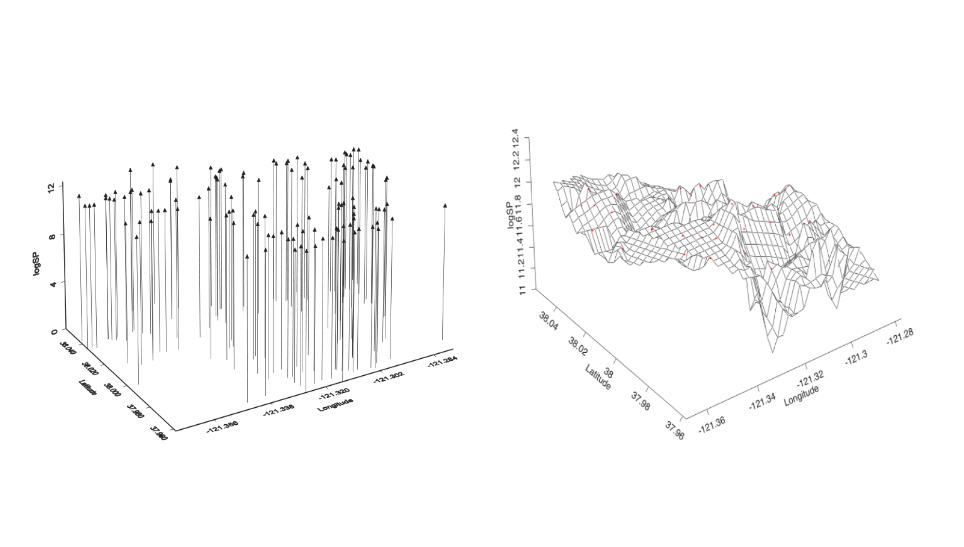
\includegraphics{images/prdprocess.png}
\caption{\label{fig:prdproc}Stockton data, Left: Spatial Lat and Long points pojected into the \(3^{rd}\) dim \(\log(Price)\), Right: spatial interpolation of points, source \citet{Blangiardo-Cameletti}}
\end{figure}

The first step in defining a spatial model within the Bayesian framework is to identify a probability distribution for the observed data. Usually are drawn distributions from the \emph{Exponential family}, indexed by a set of parameters \(\boldsymbol\theta\) as in \ref{LGM}, accounting for the spatial correlation --- note that for the sake of simplicity we slightly abuse the notation and index the generic spatial point or area by using just the subscript \(i\), rather than the indicator \(s_i\), in the following.
In the case of geostatistical data, the model parameters \(\boldsymbol\theta\), folllwing notation imposed in chapter \ref{inla} are defined as a latent stationary Gaussian Process (GP). The GP theoretical foundations and the spatial intuition are offered as a companion in the appendix \ref{gpbasics}.

\begin{definition}[GP definition]
\protect\hypertarget{def:GP}{}{\label{def:GP} \iffalse (GP definition) \fi{} }A collection of \(n\) random variables, such as \(Y(s_{1}), Y(s_{2}) , \ldots, Y(s_{n})\) that are \emph{valid} and \emph{finite} stochastic processes are said to be a \textbf{GP} if for any set of spatial index \(n\) and for each set of corresponding locations \(\left\{y\left(s_{1}\right), \ldots, y\left(s_{n}\right)\right\}\) follows a \emph{multivariate Gaussian} distribution with mean \(\boldsymbol{\mu}=\left\{\mu\left(s_{1}\right), \ldots, \mu\left(s_{n}\right)\right\}\) and covariance matrix \(\mathbf{Q}^{-1}_{i,j}, \forall i \neq j\) defined then by a covariance function \(\mathscr{\cdot, \cdot}\)
\end{definition}

The latent GP are in function of some hyper-parameters \(\boldsymbol\psi\) and their respective prior \(\pi(\boldsymbol\psi)\). Moreover a GP is completely characterized by a mean \(\boldsymbol{\mu}=\left(\mu_{1}, \ldots, \mu_{n}\right)^{\prime}\) and a spatially structured covariance matrix \(\boldsymbol{Q^{-1}}\) as multivariate Normal distribution, whose generic element is \(\boldsymbol{Q^{-1}}_{i j}=\operatorname{Cov}(\theta_{i}, \theta_{j})=\sigma^2_{\mathscr{C}} \mathscr{C}(\Delta_{i j})\), where \(\sigma_{\mathscr{C}}^{2}\) is the variance component and for \(i, j = 1, \ldots, n\). \(\mathscr{C}\left( \cdot, \cdot \right)\) function generally ensures that all the values that are close together in input space will produce output values that are close together, by inheriting the \emph{validity} and \emph{positive definitness} characteristics from the GP. Given the nature of spatial process, the covariance function has to satisfy the property of \textbf{Isotropy}.
A process is said to be \textbf{Isotropic} if the covariance function depends only on the between-points distance \(\Delta_{i j}=\left\|s_{i}-s_{j}\right\|\) (in this context \emph{Euclidean}), so it is invariant under \emph{rotation} \citeyearpar{Krainski-Rubio}. A further way of seeing this property is that Isotropy implies concentric decaying contours \citep{LecturePaci}, green in \ref{fig:isoovsanis}, that implies the vanishing of spatial dependence \citep{Blangiardo-Cameletti}, and so for covariance values.

\begin{figure}
\centering
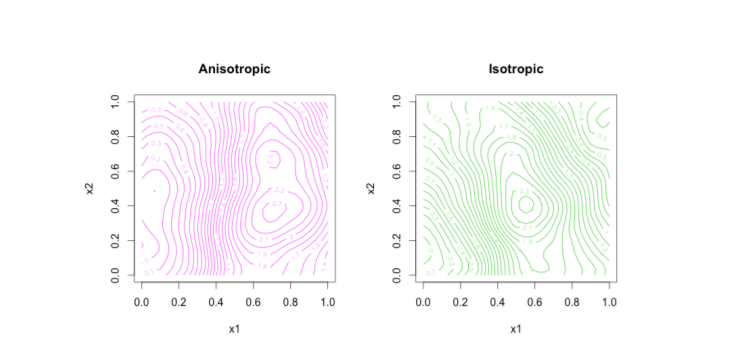
\includegraphics{images/isotropyVSanisotropy.png}
\caption{\label{fig:isoovsanis}Left: isotropy concentric decaying contours, Right: anisotropy concentric decaying contours, source \citet{blanchetscalliet}}
\end{figure}

In spatial statistics the assumption of isotropy is very frequent despite being restrictive for describing the rich variety of interactions that can characterize spatial processes. Anyway assuming the property it offers a wide range of underlying functions that can model spatial dependence for which three are the most common ones \citep{Krainski2018}, where all the parameters below are special quantities derived from the emphirical covariance function. \emph{(qui puoi aggingere le grandezze delle robe sotto)}

\[
\begin{aligned}
&\text { Exponential } \quad \mathscr{C}(\mathbf{ \Delta_{i j}})=\left\{\begin{array}{cl}
\tau^{2}_{\mathscr{C}}+\sigma^{2}_{\mathscr{C}} & \text { if }  \Delta_{i j}=0 \\
\sigma^{2}_{\mathscr{C}} \exp (-\phi_{\mathscr{C}} \Delta_{i j}) & \text { if } \Delta_{i j}>0 
\end{array}\right.\\
&\text { Gaussian } \quad \mathscr{C}(\mathbf{ \Delta_{i j}})=\left\{\begin{array}{cl}
\tau^{2}_{\mathscr{C}}+\sigma^{2}_{\mathscr{C}} & \text { if } \Delta_{i j}=0 \\
\sigma^{2}_{\mathscr{C}} \exp \left(-\phi^{2}_{\mathscr{C}}  \Delta_{i j}^{2}\right) & \text { if } \Delta_{i j}>0 
\end{array}\right. \\
&\text { Matérn } \quad \mathscr{C}(\mathbf{ \Delta_{i j}})=\left\{\begin{array}{cl}
\tau^{2}_{\mathscr{C}}+\sigma^{2}_{\mathscr{C}} & \text { if } \Delta_{i j}=0 \\
\frac{\sigma^{2}_{\mathscr{C}}}{2^{\nu-1} \Gamma(\nu)}(\phi_{\mathscr{C}}  \Delta_{i j})^{\nu} K_{\nu}(\phi_{\mathscr{C}}  \Delta_{i j}) & \text { if } \Delta_{i j}>0
\end{array}\right.
\end{aligned}
\]

In particular the focus is on the \emph{Matérn} -- as it is required by the SPDE approach in Section \ref{spdeapproach} -- and this should not be intended as a restriction. In fact, as described in Guttorp and Gneiting (2006) \emph{miss lit}, the Matèrn family is a very flexible class. Matérn is tuned mainly by two hyper-parameters, a scaling one \(\kappa>0\), usually set equal to the range \(\sigma_{\mathscr{C}}^{2}\) i.e.~the distance at which the spatial dependece becomes negligible, by the relation \(\sigma_{\mathscr{C}}^{2}=\frac{\sqrt{8 \lambda}}{\kappa}\)), and a smoothing one \(\nu>0\). A \emph{isotropic} Matérn covariance expression is obtained by isoltating the \(\sigma_{\mathscr{C}}^{2}\), the variance component \citep{Cressie_2015}:

\[
\mathscr{C}\left(\Delta_{i j}\right)=\frac{1}{\Gamma(\lambda) 2^{\lambda-1}}\left(\kappa \Delta_{i j}\right)^{\lambda} K_{\lambda}\left(\kappa \Delta_{i j}\right)
\]
\(\Gamma(\nu)\) is a Gamma function depending on \(\nu\) values, \(K_{\nu}(\cdot)\) is a modified Bessel function of second kind. The smoothness parameter \(\nu\) in figure \ref{fig:matern} takes 4 different values showing the flexibility of Matérn to relate distances acording to varyinn parameters. When \(\nu = 1\) \ldots{} When \(\nu = 1/2\) it becomes the exponential covariance function, When \(\nu = 3/2\) it uncovers a convenient closed form \citep{LecturePaci}, when \(\nu \approx \infty\), e.g.~for graphical constraints \(\nu = 80\), it becomes Gaussian covariance function. In the the case shown in section \ref{spdeapproach} \(\sigma_{\mathscr{C}}^{2}\) range is set equal to the distance at which dependence vanishes below .1, for any \(\lambda\).

\begin{figure}
\centering
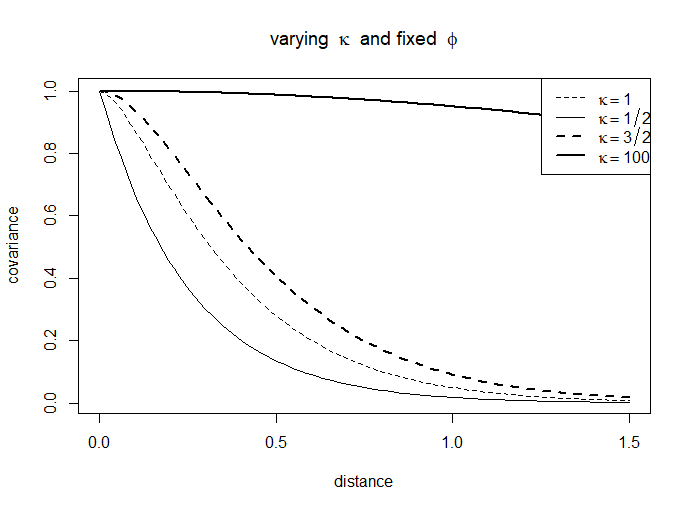
\includegraphics{images/matern.png}
\caption{\label{fig:matern}Matérn function with 4 different values of \(\nu\) (upper right legend), kept \(\phi\) fixed, author's source}
\end{figure}

\textless!--
\textless!--
\textless!--
\textless!--

\hypertarget{spdeapproach}{%
\section{The Stochastic Partial Differential Equation (SPDE) approach}\label{spdeapproach}}

Locations in the spatial setting are considered as realizations of a stationary, isotropic unobserved GP \(w(s)\) to be estimated (\ref{GP}). Before approaching the problem with SPDE, GPs were treated as multivariate Gaussian densities and Cholesky factorizations were applied on the covariance matrices and then fitted with likelihood \citep{LecturePaci}. Covariance matrices in the context of spatial and spatio-temporal models \citep{PACI2017149, Cameletti2012} are \(n \times n\) whose dimension is produced the number of observations at each single location (at each time point in spatio-temporal) \citep{BLANGIARDO201339}. Covariance matrix as such are very dense and they were scaling with the order of \(\mathcal{O}\left(n^{3}\right)\) \citep{Banerjee-Gelfand}. Problem were linked to the computational costs needed for linear algebra operations for model fitting and spatial interpolation as well as prediction \citep{Cameletti2012}, having led to obvious \emph{big-n} problem.
The breakthrough came with \citet{Lindgren2011} that proves that a stationary, isotropic (might be relaxed) GP with Matérn covariance can be represented as a GMRF using SPDE solutions by finite element method \citep{Krainski-Rubio}. In other words given a GP whose covariance matrix is \(\boldsymbol{Q^{-1}}\), SPDE can provide a method to approximate \(\boldsymbol{Q^{-1}}\) without the previous computational constraints. As a matter of fact SPDE are equations whose solutions are GPs with a chosen covariance function focused on satisfying the relationship SPDE specifies \citeyearpar{Krainski-Rubio}.
Benefits are many but the most important is that the representation of the GP through a GMRF provides a sparse representation of the spatial effect through a sparse precision matrix \(\boldsymbol{Q}\) . Sparse matrices enable convenient inner computation properties of GMRF \ref{approx} which are exploited by INLA algorithm \ref{inla} leading to a more feasible big-O \(\mathcal{O}\left(n^{3 / 2}\right)\). Mathematical details and deep understanding of the equations in SPDE are beyond the scope of the analysis. Luckily enough R-INLA has a set of functions that makes clear to the practitioner the minimal requirements to pass from discrete locations to their continuously indexed surface alter-ego.
In few words SPDE approach uses a finite element (FEM method) representation to shape the Matérn field as a linear combination of basis functions defined on a triangulation of the domain \(\mathcal{D}\) \citeyearpar{Cameletti2012}. What it intenally does is splitting the domain \(\mathcal{D}\) into a number of non-intersecting triangles which converge in a common edge or corner. Then the initial vertices of the triangles are set at \(s_1 \ldots s_d\). In order to get a proper triangulation, useful for spatial prediction, additional vertices are then added. The more vertices are added the more the triangulation is accurate since many more triangles can better interpolate the surface reaching more complex shapes. Secondly SPDE projects the values of the trinagularization to the dicretized spatial surface with weighted sum of areas of the underlying triangles. A less superficial intuition is offered in the appendix in section \ref{triangular} on how SPDE computes triangularized valuez and how it projects the triangulation to the GRMF.\\
To illustrate the concept of triangulation \citet{Cameletti2012} provide a simple example for Piemonte PM10 concentration observed at 24 monitoring stations left in figure \ref{fig:piepm10} and using 123 vertices and a Piemonte borders, right in figure \ref{fig:piepm10}.

\begin{figure}
\centering
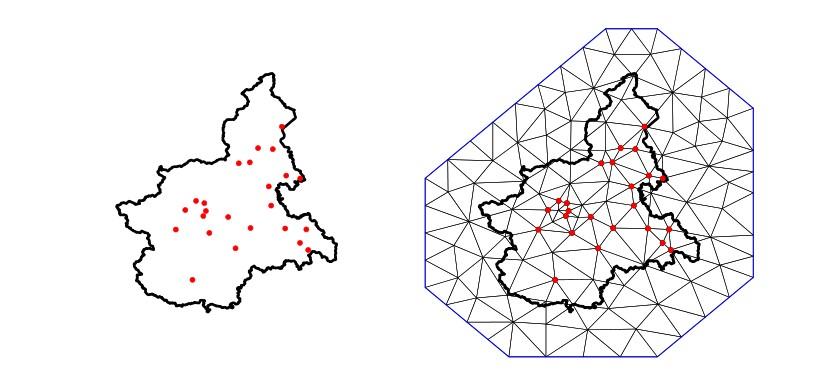
\includegraphics{images/piemonte_pm10.jpg}
\caption{\label{fig:piepm10}Left: monitoring stations in Piemonte region for PM10 pollution levels. Right: its triangulation using 123 vertices. \citet{Cameletti2012} source}
\end{figure}

Any triangle height (the size of the spatial field at each vertix triangle) is calculated by weighted sum, with linear interpolation deciding the values within the triangle. Figure \ref{spdesurf} shows a continously indexed random spatial field (left side of figure \ref{spdesurf}) with the corresponding SPDE on the basis of a triangulation (right panel \ref{spdesurf}).

\begin{figure}
\centering
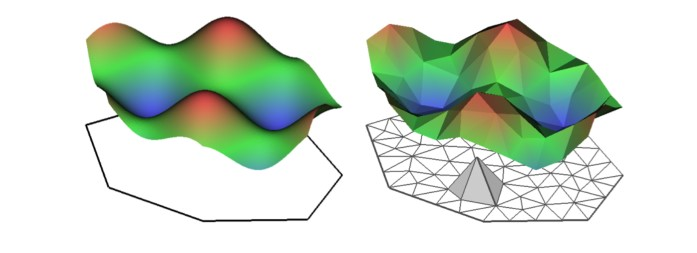
\includegraphics{images/spde_indexedsurface.jpg}
\caption{\label{fig:spdesurf}Left: example of a spatial random field where \(X(s)= \cos(s_1)+\sin(s_2)\), Right: \(X(s)\) SPDE representation given a triangulation, \citet{Cameletti2012} source}
\end{figure}

\hypertarget{hedonic-rental-price-models}{%
\section{Hedonic (rental) Price Models}\label{hedonic-rental-price-models}}

The theoretical foundation of the Hedonic Price Models (from now on HPM) resides in the consumer utility theory of \citet{Lancaster} together with \citet{Rosen} market equilibrium. According to Lancaster the utility of a commodity does not exist by itself, instead it exists as the sum of the utilities associated to its separable characteristics. Integrating Lancater, Rosen introduces HPM and suggests that each separate commodity characteristics are priced by the markets on the basis of supply and demand equilibra. Applying HPM to Real Estate in a market context, from the buy side house prices (indeed also rents) are set as the unit cost of each household attributes, conversely from the selling side the expenditures associated to build of each them.
Formalizing the results, Hedonic Price \(P\) in Real Estate is expressed as a general \(f\) functional form that takes as input the house characteristics vector \(\mathbf{C} = \{c_1,c_2, c_3, \ldots c_n\}\).

\[P=f\left(c_{1}, c_{2}, c_{3}, \ldots, c_{n}\right)\]

Vector \(\mathbf{C}\) since now might contain a unidentified and presumably vast number of ungrouped characteristics. In this setting \citet{Malpezzi} tried to organize house features by decomposing \(\mathbf{C}\) into mutually exclusive and exhaustive subgroups. The vector components involves the house price \(P\), which is in a \(f\) relation with: \(S\), the structural characteristics of the house, \(N\), the neighborhood characteristics, \(L\), the locational characteristics, \(C\), the contract conditions and \(T\) time dimension (not included in the model). \(\beta\) is the vector of the parameters to be estimated. Therefore:

\[P=f\left(S, N, L, C, T, \beta\right)\]
However the critical part of studying house characteristics in geostatistics is the \emph{estimation} and a recent (and not recent) number of emerging trends are observed \citep{SHEPPARD19991595}. Trends, other than the methods presented in this analysis suggests semi-parametric or non-parametric methods and applications of spatial econometrics \citet{Ling}. Researchers would also contend with problems ranging from variable selection to model specification \citeyearpar{Ling}.
For semi-paramametric models a local polynomial regression is developed by \citet{clapp}. The model provides a nonlinear term for the measurement of housing position values dependent on latitudes and longitudes.
Proper geoadditive models family was originally proposed by Kammann and Wand \citeyearpar{kammanwand}, which offers a combination of additive modeling \citep{buja1989} and a geostatistical component. As Ling \citeyearpar{Ling} points out the candidates for the spatial component are many, e.g.~kriging component \citep{dey2017metamodel} (which will be then subsituted with a GP \ref{GP}) or a smooth spatial trend component based on a tensor product of longitude and latitude for which \citet{basilebenfratmcast} have investigated European industrial agglomeration externalities. The model outshines the other parameteric model performances by better managing spatial unobserved patterns. Furthermore they made available a third study dimension which is time \citeyearpar{Ling}.
Spatial econometrics' evolution trends are seen in \citet{spateconomshifei} and lately in \citet{spateconanslein} where point referenced data are modeled with endogenous time varying spatial weights matrices and unobserved common factors and ultimately are fitted with traditional bayesian estimation methods as MCMC \citeyearpar{spateconanslein}.
Then two further interesting modeling approach does not fall perfectly in the categories, but are higly considered in literature within the Hedonic Price models. \citet{dubelegros} recognize that the modeling tools available analyzing point referenced data were not sufficient to take into account all the dimensions according to which they want to evaluate the phenomenon. They acknowledge that \emph{Moran's I} index and his statistics test relies mainly on an exogenous specification of a spatial weights matrix \citeyearpar{dubelegros}. As a result they assemble a spatio‐temporal weights matrix to evaluate spatial dependence through Moran's I index whose application is on real estate data (selling) for Québec City from 1986 to 1996. The second approach was addressed in \citet{baltagiparis} whose object is price estimation based on flats sold in the city of Paris over the period 1990--2003. This is a rich and unbalanced pseudo‒panel data which are modeled with spatial lag. Results displayed a nested structure of the Paris housing data, which have been tested with likelihood ratio. A similar approach was followed by Nardelli and Arbia \citep{arbia2020spatial} which collected crowdsourced as well as webscraped (as in section \ref{scraping}) data and lately applied Spatial Lag Model (SLM) on a ``post-sampled'' \citep{arbia2020postsampling} version of the same. As a result bias in the model is diminished, indeed variance of the estimators is increased.
A further aspect of the problem is posed by scholars that do not consider rents to be representative for the actual value of real estate, as a result modeling choices should be calibrated on the market economic cricumstances. Nevertheless in many empirical analysis rent value are considered a proxy for real estate pricing when considered in long-run \citep{Herath_Maier_2011}. A further argument to endorse this hypothesis is brought by \citet{sellingVSrental} considering housing a commodity, then the selling or the rental option should be considered interchangeable economic actions with respect to same inner need to be satisfied. This assumption is also stronger in this context since Manganelli, Morano, and Tajani have centered their analysis on italian Real Estate data. Moreover \citet{Capozza_Seguin_1996} discussed on how much rent-price ratio predicts future changes both in rents and prices. Among all the other points raised they brought the decomposition of rent-price ratio into two parts: the predictable part and the unexplained residuals part. The predictable part was discovered to be negatively correlated with price changes, in other words cities in which prices are relatively high with respect to rents are associated with higher capital gains that might justify that misalignment. This is also true for the opposite, that is cities in which prices are lower with respect to the rents, and this effect can not be associated to any local condition, realize lower capital gains. A further argument is offered by Clark \citep{Clark_1995} which went after the Capozza and Seguin work. Rent-price ratio is negatively correlated with following future changes in rents. In other words prices are still higher when areas in which they are observed documents an increase in rent prices.

\hypertarget{univariateregr}{%
\section{Point Referenced Regression for univariate spatial data}\label{univariateregr}}

Since in HPM the relationships between the characteristics of the house, i.e.~vector \(\mathbf{C}\) and the price \(P\) is not in any case fixed by econometric literature it is possible to assume any \(f\) functional form. The open possibility to apply a wide range of relationship between covariates fit in the INLA setting, since Latent Gaussian Models are prepared to accept a any linear and non linear \(f\) functions \ref{LGM} through the \passthrough{\lstinline!f()!} method. Hedonic price models are, as a consequence, a subset of models that can be fitted into LGM and therefore by INLA method.

Moreover what the vast majority of econometric literature \emph{(Greene, 2018)} suggest to apply a is log-linear / square root model. This is due to the fact that log transformation / square root smooths the skewness of prices normalizing the curve, leading to more accurate estimates. Having an exponential family generating process lowers even further computational cost for reasons linked to the \(\tilde\pi(\boldsymbol{\psi})\) hyper param INLA approximation \citep{Blangiardo-Cameletti}. Notation is taken from the previous chapter \ref{inla}, for brevity purposes \(\boldsymbol{\beta}\) \(\mathbf{X}\) and \(\boldsymbol{y}\) indicates vectors incorporating all their respective realizations and the \(s\) spatial component is left out in favor of the observation pedix \(i\).\\
The simplest log-linear bayesian regression model assumes linear relationship between predictors and a Normal data generating process: (log has been taken out for simplicity, bu it will be then considered in the regression setting) (valuta l'idea che per interpretabilità di modellarla come Gamma exponential family anzichè tenerla normale)

\[
\log{(y_{i})} \sim \operatorname{Normal}(\mu_{i}, \sigma^{2})
\]

\[
y_{i}=\mu_{i}+\varepsilon_{i}
\]

then by the following relationship \(E\left(y_{i} \mid \beta_{0}, \ldots, \beta_{M}, x_{i 1}, \ldots, x_{i M}\right)=\beta_{0}+\sum_{m=1}^{M} \beta_{m} x_{i m}\) it is possible to specify a more general linear predictor (seen also in chapter \ref{inla}) through an identity link function i.e.~\(\eta_{i}=g\left(\mu_{i}\right)=\mu_{i}\) obtaining:

\[
\eta_{i}=\beta_{0}+\sum_{m=1}^{M} \beta_{m} x_{m i}+\sum_{l=1}^{L} f_{l}\left(z_{l i}\right)
\]

Where, once again, the mean structure linearly depends on some \(\mathbf{X}\) covariates, \(\boldsymbol{\beta}\) coefficients, \(f_{l}(\cdot), \forall l \in 1 \ldots L\) are a set of random effects defined in terms of a \(\boldsymbol{z}\) set of covariates \(\boldsymbol{z}=\left(z_{1}, \ldots, z_{L}\right)\) (e.g.~rw, ar1) and \(\varepsilon_{i}\) white noise error.
Priors have to be specified and a non informativeness for \(\tau^2 = 1/\sigma^2\) and \(\boldsymbol{\beta}\) is chosen, such that \(\pi(\tau^2) \propto 1\) and \(\pi(\boldsymbol\beta) \propto 1\). As a consequence the conditional posterior for the parameters of interest \(\boldsymbol{\beta}\) is:

\[
\boldsymbol{\beta} \mid \sigma^{2}, \boldsymbol{y}, \boldsymbol{X} \sim \operatorname{MVNormal}\left(\left(\boldsymbol{X}^{\prime} \boldsymbol{X}\right)^{-1} \boldsymbol{X}^{\prime} \boldsymbol{y}, \sigma^{2}\left(\boldsymbol{X}^{\prime} \boldsymbol{X}\right)^{-1}\right)
\]

where the mean structure corresponds to the OLS estimator: \(\left(\boldsymbol{X}^{\prime} \boldsymbol{X}\right)^{-1} \boldsymbol{X}^{\prime} \boldsymbol{y}\) for \(\beta\) and then to obtain the marginal posterior for \(\boldsymbol{\beta}\) it is needed to integrate with respect to \(\sigma^2\).

In order to engage the spatial coordinate components into the regression setting \(w_{i}\) has to be added to the equation. \(w_{i}\) is set as a stationary and isotropic GP with mean 0 and variance as covariance function expressed as Matérn.
Recall that GP
The new regression setting integrates the \emph{spatial error} part in the name of \(w_{i}\) and a \emph{non-spatial error} part \(\varepsilon_{i}\) distributed normally with mean 0 and variance \(\tau^2\) ,i.e.~\(\mathrm{N}\left(0, \tau^{2}\right)\), which offers its contribution error to the nuggets via the covariance function.
Consequently there is one more parameter to estimate. It is worth mentioning that the distribution of \(w_{i}\) at a finite number of points is considered a realization of a multivariate Gaussian distribution. In this case, the likelihood estimation is possible and it is the multivariate Gaussian distribution with covariance \(\Sigma\).

\[
\log(y_{i})= \beta_{0} + (\mathbf{X})^{\prime}\boldsymbol{\beta}+w_{i}+\varepsilon_{i}
\]

The covariance of the marginal distribution of \(y_{i}\) at a finite number of locations is \(\Sigma_{y} = \Sigma + \tau^2\mathbf{I}\), where \(\mathbf{I}\) denotes the indicator function (i.e., \(\mathbf{I}(i = i^{\prime})= 1\) if \(i = i^{\prime}\), and 0 otherwise). This is a short extension of the basic GF model, and gives one additional parameter to estimate

\begin{equation}
    \log(y_{i})=\mu_{i}+\varepsilon_{i}
\label{eq:genreg}
\end{equation}

where \(y_{i}\) is normally distributed as \(y_{i} \sim \operatorname{Normal}\left(\mu_{i}, \sigma^{2}\right)\) and \(\mu_{i}\) is the mean structure that linearly depends on some \(\mathbf{X}\) covariates, \(\boldsymbol{\beta}\) coefficients, \(f_{l}(\cdot), \forall l \in 1 \ldots L\) are a set of random effects defined in terms of a \(\boldsymbol{z}\) set of covariates \(\boldsymbol{z}=\left(z_{1}, \ldots, z_{L}\right)\) (e.g.~rw, ar1) and \(\varepsilon_{i}\) white noise error. Please recall that the \(i\)th pedices are the observations and the \(m\)th pedices are the covariates. The structure is a repetition of what already seen in chapter \ref{LGM}

\begin{equation}
  \eta_{i}=\beta_{0}+\sum_{m=1}^{M} \beta_{m} x_{m i}+\sum_{l=1}^{L} f_{l}\left(z_{l i}\right)
\label{eq:linearpred}
\end{equation}

The link function specified in this case is still identity, so that \(\eta_{i}=g\left(\mu_{i}\right)=\mu_{i}\). Nevertheless GLMs can be applied with different link function. when response variable has to stay between \([0,1]\) (e.g.~probabilities), the link function might be Logit, which leads to logistic regression. More generally expressed in vector notation:

\begin{equation}
  \log(y_{i})\left(\mathbf{s}_{i}\right)=\mathbf{x}\left(\mathbf{s}_{i}\right)^{\prime} \beta_{j}+\varepsilon\left(\mathbf{s}_{i}\right)
  \label{eq:genregvec}
\end{equation}

where its OLS estimator is:
\begin{equation}
  \hat{\beta}=\left(\mathbf{X}^{\prime} \mathbf{X}\right)^{-1} \mathbf{X}^{\prime} \mathbf{y}
\label{eq:ols}
\end{equation}

Moreover In the context of bayesian analysis a prior distribution has to be imposed on the regression coefficients \(\beta = \left\{\beta_{0}, \ldots, \beta_{J}\right\}\) as well ad on the variance \(\sigma^{2}\) of \(y_{i}\). When no expert information is provided vague priors are introduced, meaning that the regression should not be weighted too much on the priors choice.
Vague priors might be:

\begin{itemize}
\tightlist
\item
  \(\beta_{m} \sim \operatorname{Normal}\left(0,10^{6}\right)\) for the beta coefficients
\item
  \(\log (\tau)=\log \left(1 / \sigma^{2}\right) \sim \log \operatorname{Gamma}\left(1,10^{-5}\right)\) for precision
\end{itemize}

Spatial modeling goal is to include spatial information from location into the model. This is done within the bayesian frameoùwork and INLA by adding \(w(\mathbf{s})\) in the previous equation \eqref{eq:genregvec}.

\[y\left(\mathbf{s}_{i}\right)=\mathbf{x}\left(\mathbf{s}_{i}\right)^{\prime}\beta_{j}+w(\mathbf{s})+\varepsilon\left(\mathbf{s}_{i}\right)\]

The \(w(\mathbf{s})\) in the context of the analysis is approached as a stationary and isotropic GP\ref{GP} whose distribution by definition is multivariate Gaussian with mean \(\boldsymbol{\mu}(\mathbf{s}) = 0\) and function of the spatial index \(\mathbf{s}\) and covariance function \(\mathcal{C}( \cdot \mid \theta)\) .
\(\varepsilon(\mathbf{s})\) is iid and mean centered in 0 with variance \(\tau^{2}\) and is called non-spatial error since it contributes to the nugget. The error term is pure since it interferes with the covariance function so that the model can embody the spatial component.
One of the major advantages of having a a spatial process embedded into a GP is \emph{likelihood} based inference.

\hypertarget{parameter-estimation}{%
\subsection{Parameter estimation}\label{parameter-estimation}}

Gaussian spatial models can be considered as GLM with a particular specification of the precision matrix \(\Sigma_{\theta}=\sigma^{2} \mathbf{R}(\phi)+\tau^{2} I_{n}\),
then the likelihood can be computed by:
\[\mathbf{y} \mid \boldsymbol{\theta}, \boldsymbol{\beta} \sim \mathrm{N}\left(\mathbf{X} \beta, Q_{\theta}\right)\]
where, \(\boldsymbol{\theta}=\left(\sigma^{2}, \tau^{2}, \phi\right)\)
Since likelihood estimation is possible then MLE can be computed for \(\boldsymbol{\beta}\) and \(\boldsymbol{\theta}\) are \(\hat{\boldsymbol{\beta}}\) and \(\hat{\boldsymbol{\theta}}\).
Then the estimation in vector notation is:

\[\hat{\boldsymbol{\beta}}_{M L E}=\left(\mathbf{X}^{\prime} Q^{-1} \mathbf{X}\right)^{-1} \mathbf{X}^{\prime} Q^{-1} \mathbf{y}\]

\hypertarget{kriging}{%
\section{Spatial Kriging (prediction)}\label{kriging}}

In Geostatistics the main interest resides in the spatial prediction of the spatial latent field pr the response variable at location not yet observed.
Assumed the model in the previous section, suppose that \(y^{\star}\) is not a observed occurrence of the response variable at location \(s_{0}\) (not in the data) of the GP \(w_{i}\) spatial surface estimated through observed refereced points in \(\boldsymbol{y}\). As a consequence of exchangeability (first step previous section @ref(inlahier )) then \(\boldsymbol{y}^{\otimes}=\left\{\boldsymbol{y}, y^{\star}\right\}\). Then considering INLA notation it is obtained:

\[
\begin{aligned}
&\pi\left(y^{\star} \mid \boldsymbol{y}\right)=\frac{\pi\left(\boldsymbol{y}, y^{\star}\right)}{\pi(\boldsymbol{y})} \text { from the conditional probability }\\
&=\frac{\int \pi\left(y^{\star} \mid \theta\right) \pi(\boldsymbol{y} \mid \theta) \pi(\theta) \mathrm{d} \theta}{\pi(\boldsymbol{y})} \text { by exchangeability }\\
&=\frac{\int \pi\left(y^{\star} \mid \theta\right) \pi(\theta \mid y) \pi(y) \mathrm{d} \theta}{\pi(y)} \text { applying Bayes' theorem }\\
&=\int \pi\left(y^{\star} \mid \boldsymbol{\theta}\right) \pi(\boldsymbol{\theta} \mid \boldsymbol{y}) \mathrm{d} \boldsymbol{\theta}
\end{aligned}
\]

A DAG representation might offr the intuition behind Prediction in spatial models:

\begin{figure}
\centering
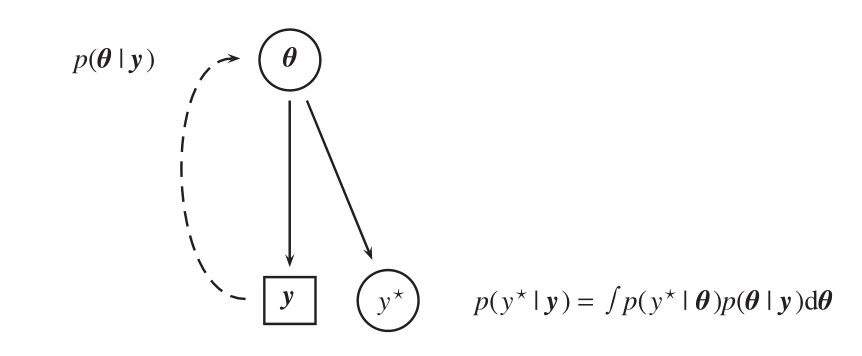
\includegraphics{images/spatial_prediction.jpg}
\caption{Spatial prediction representation through DAG, source \citet{Blangiardo-Cameletti}}
\end{figure}

where \(\pi\left(y^{\star} \mid \boldsymbol{y}\right)\) is said predictive distribution and it is meaningful only in the Bayesian framework since the posterior distribution is treated as a random variable, which is totally not true in frequentist statistics.

\hypertarget{model-checking}{%
\section{Model Checking}\label{model-checking}}

Once the model is set up and fitted a resampling scheme has to be chosen in order to evaluate the model performance. One of the most used method to assess beyasian model quality is LOOCV cross validation and defualt choice fo R-INLA package. From data is left out one single observation and so that the Validation set is \(\boldsymbol{y}_{v} = \boldsymbol{y}_{-i}\) and the Assessement set is a \(\boldsymbol{y}_{a} = \boldsymbol{y}_{i}\)
the rest of the observations. Two KPI are assumed to be representative:

\begin{itemize}
\tightlist
\item
  CPO conditional predictive ordinate (pettit, 1990): \(CPO_{i} = \pi(y^{\star} \mid \boldsymbol{y}_{v})\)
\item
  PIT probability integral tranform (dawid, 1984): \(PIT_{i} = \pi(y^{\star} < y_{i} \mid \boldsymbol{y}_{v})\)
\end{itemize}

These quantities are used by default by setting control options in the \passthrough{\lstinline!inla(control.compute = list())!} list object by setting them equal o TRUE. Inla also provides an inner method to authomatically handlee failing in computing those two quantities, leadind to values of 1 when predictions are not reliable and the ipposite for 0.Moreover the empirical distribution of the PIT can be used to asses predictive performance: if it is Uniform, so there are not values that strongly differ from the others then the model is correctly checked. Otherwise if the dostribtuon almost approxiamtes any of the other possibles then the Cross validation assessement prediction has led incorrectly predict the ``out of the bag'' validation sample.

Posteerior checking method exploits a full cross validation where \(\boldsymbol{y}_{a} = \boldsymbol{y}_{v}\) and it is called predictive checks. Th assessement set now is equal to the validation set,a s a consequence all the observation are evaluated twice. 4 quantities are driver to model estimate quality:

\begin{itemize}
\tightlist
\item
  the \emph{posterior predictive distribution}: \(\pi(y^{\star} \mid \boldsymbol{y}) = \int \pi(y^{\star} \mid \theta_{i})\pi({\theta_{i}} \mid \boldsymbol{y})\mathrm{d}\theta_{i}\) which is the likelihood of a replicate observation. When values are small that indicates that are those values are coming from tails, since the area under the curve (i.e.~probability) is less. If this happens for many observation then outliers are driving the model leading to poor estimates
\item
  the \emph{posterior predictive p-value} whose math expression is:\(\pi(y^{\star} \leq y_{i} \mid \boldsymbol{y})\) for which values near to 0 and 1 indicates poor perfomances.
\item
  \emph{Root Mean Square Predictive Error RMSE}: \(\sqrt{\frac{1}{n} \sum_{i=1}^{n}(y_{i}-{y}^{\star}_{i})^{2}}\)
\item
  \(R^2\)
\end{itemize}

R-INLA has already antiticipated in chapter 4 section\ref{example} have designed function to compute statistics on posterior distribution as \passthrough{\lstinline!inla.pmarginal()!} returning the cumulative density distribution.

\hypertarget{prior-specification}{%
\section{Prior Specification}\label{prior-specification}}

\hypertarget{spde}{%
\chapter{SPDE approach}\label{spde}}

Observations in the spatial problem setting are considered as realizations of a stationary, isotropic unobserved GP \(w(s)\) that we aim to estimate (\ref{GP}). Before approaching the problem with SPDE, GPs were treated as multivariate Gaussian densities and Cholesky factorizations were applied on the covariance matrices and then fitted with likelihood. Matrices in this settings were very dense and they were scaling with the order of \(O\left(n^{3}\right)\), leading to obvious big-n problem.
The breakthrough, came with \citet{Lindgren2011} that proves that a stationary, isotropic GP with Matérn covariance can be represented as a GMRF using SPDE solutions by finite element method \citep{Krainski-Rubio}. In other words given a GP whose covariance matrix is \(\boldsymbol{Q}\), SPDE can provide a method to approximate \(\boldsymbol{Q}\) without computational constraints. As a matter of fact SPDE are equations whose solutions are GPs with a chosen covariance function focused on satisfying the relationship SPDE specifies.
Benefits are many but the most important is that the representation of the GP through a GMRF provides a sparse representation of the spatial effect through a sparse precision matrix \(\boldsymbol{Q}^-1\) . Sparse matrices enable convenient inner computation properties of GMRF that can be exploited with INLA. Bayesian inference on GMRF can take advantage of lower computational cost because of these properties stated before leading to a more feasible big-O \(O\left(n^{3 / 2}\right)\). The following chapter will provide a intuition on SPDE oriented to practitioners. The chapeter once again will follow the track of Krainski \& Rubio \citeyearpar{Krainski-Rubio} and Blangiardo and Cameletti \citeyearpar{Blangiardo-Cameletti} works, together with the street-opener paper from \citet{Miller2019} as compendium. SPDE might be complex for those who are not used to applied mathematics and physics making it difficult not only to grab the concept, but also to find its applications. One more obstacle regards SPDE software implementation, since without deep technical expertise it might be difficult to customize code with the aim to extend the methodology to different models. For a gentle introduction on what a SPDE is from a mathemathical perspective a valuable reference is \citet{Miller2019} in secction 2.1, then also its application to Matérn in 2.3.

\hypertarget{set-spde-problem}{%
\section{Set SPDE Problem}\label{set-spde-problem}}

Given the statistical model already encountered in chapter \ref{univariateregr}:

\[
y\left(\mathbf{s}_{i}\right)=\mathbf{x}\left(\mathbf{s}_{i}\right)^{\prime} \beta_{j}+w(\mathbf{s})+\varepsilon\left(\mathbf{s}_{i}\right)
\]

where \(\eta(\mathbf{s}_{i}) = g (\mathbf{x}\left(\mathbf{s}_{i}\right)^{\prime}\beta_{j})\) is the linear predictor, whose link function \(g( \cdot )\) is identity (can be also extended to GLM), where \(w(\mathbf{s})\) is a Gaussian Process with mean structure 0 and \(C(\cdot)\) covariance structure ( where \(\boldsymbol{Q}\) is the covariance matrix and \(Q^{-1}\) precision matrix). Then \(w(s) \sim MV\mathcal{N}(0, \boldsymbol{Q}_{i,j}^{-1})\) and where \(\varepsilon(\mathbf{s}_{i})\) is white noise error such that \(\varepsilon(\mathbf{s}_{i}) \sim \mathcal{N}\left(0, \tau^{2}\right)\).
Comprehending \(w\) in the model brings two major issues, specify a covariance function for observations as well as how to fit the model. Among all the possible reachable solutions including the SPDE, the common goal is to define covariance function between locations by approximating the precision matrix \(\boldsymbol{Q}^{-1}\), since they are an effective tool to represent covariance function as in section \ref{LGM}.
For those reasons SPDE approach implies finding an SPDE whose solution have the precision matrix, that is desired for \(w\). \citet{Lindgren2011} proves that an approximate solution to SPDE equations is to represent \(w\) as a sum of basis function multiplied by coefficients \citeyearpar{Miller2019}. Moreover the basis function coefficients are in reality a GMRF (for which fast method comptations already exists).

\hypertarget{spde-within-r-inla}{%
\section{SPDE within R-INLA}\label{spde-within-r-inla}}

First point addresses the assumption that a GP with Matérn covariance function and \(\nu >0\) is a solution to \emph{SPDE} equations.
Second point addressed the issues of solving SPDE when grids are irregular, as opposite with the one seen in first point (regular grid for irregular distribution. In here comes FEM used in mathematics and engineering application with the purpose to solve differential equations. Notation is kept coherent with the one for the previous chapter.

\hypertarget{first-point-krainsky-rubio-too-technical}{%
\section{First Point Krainsky Rubio TOO TECHNICAL}\label{first-point-krainsky-rubio-too-technical}}

A regular 2D grid lattice is considered with infinite number of location points as vertices.

\begin{figure}
\centering
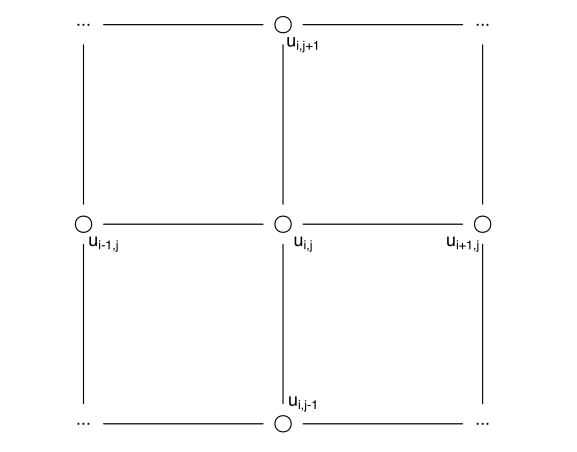
\includegraphics{images/lattice.png}
\caption{lattice 2D regular grid}
\end{figure}

\hypertarget{exploratory}{%
\chapter{Exploratory Analysis}\label{exploratory}}

Data emerging from the RESTful API body response is not in its tidiest form regardless of the query arguments sent. Yet data undergoes to a series of pre-processing step during scraping, which still requires to clear up some unnecessary character and to separate columns containing more than one covariate. To the analysis extent data should be reproducible in the sense that it should come from the same geographic area otherwise the analysis would be not comparable. As a result API parameters are kept permanent (e.g.~Milan rental real estate within ``circonvallazione'' approximated geo-borders) by passing to the API arugments \passthrough{\lstinline!.thesis!} parameter . As a consequence a dedicated endpoint is passed in the argument body. By setting the option equal to to TRUE the API caller requests thesis data. In other words the latter option under the hood secures to specify to the API an already composed query url to be passed to the scraping endppoint, which corresponds to precise zones imposed while searching for advertisemnts on Immobiliare.it. To help figure out the idea behind the operation it can be thought as refreshing everyday the same immobiliare.it url on their website looking for accomodations within a specified zone.
Parameters specified are also npages = 120, leading to to 3000 observations. The \passthrough{\lstinline!*!} refers to the EC2 public DNS.

As a further data source is available a mondgoDB ATLAS cluster which, because of the scheduler, stocks daily .csv information from Milan real estate. Credentials have to be supplied. For run time reasons also related to the bookdown files continuous building the API endpoint is not called and code chunks outputs are cached due to heavy computation. Instead data is extracted from the MongoDB cluster. A summary table of the columns involved is presented with the goal to introduce the reader to API incoming data. Data needs some heavy preprocess steps to get modeled which is briefly covered in the data preparation part in section \ref{prep}. Data coming from the /complete enndpoint has a geo-statistical spatial component and consequently a spatial representation of the dataset is showed. One further plot points out that geographic coordinates are non-linearly related \ref{fig:NonLinearSpatialRel} to the price response variable so dedicated techniques are required. Exploration starts with factor counts evidencing a ``Bilocale'' prevalence which is then compared to other cities. This suggest some critical Milan real estate market demand information and consequently reflections on the offer. Heating and cooling systems, two of the covariates extracted, are grouped and then arranged by descending order prevalence. They both do not display any significative price change but they bring to the surface an important environmental concern. The same is done by highlighting ridges distribution for other two newly engineered covariates. Data displays bimodality in prices distribution for different n-roomed accommodations and the model should take account of the behavior. Then a piece-wise linear regression is fitted for each n-roomed accommodation sub-group whose single predictor is the square meter footage. The analysis emphasize some valuable economic consequences both for investors interested into property expansions and for tenants that are planning to partition single properties into rentable sub-units. The previous analysis brings along a major question which regards the most valuable properties per single square meter surface and a answer based on data is given. Then a further log linear regression setting is proposed to evaluate the impact of some other presumably important covariate. A Tie Fighter plot displays for which coefficient, associated to each dummyied predictor, there are surprisingly high prices compared to the effect of the square meter footage expansion. A partial conclusion is that having 2 or 3 bathrooms truly pays an extra monthly gain, also caused by the number of tentants the accomodations could host. Then missing assessement and imputation takes place. At first is made a brief a revision of missing and randomnes by \citet{Little}, then theory is applied by visualizing missing in combination with heat-map and co-occurrence plot. Combined missing observation test is able to detect whether data is missing because of inner scraping faiilures or simple rarity in data appereance. Then for the observations that passed the test imputation is made through INLA posterior expectation. That is the case of data lost in predictors so the missing covariates ( \emph{condominium} ) are brought into a model as response variable whose this time predictors are explanatory ones. Through a method specified within the INLA function the posterior statistics are computed and then finally imputed in the place of missing ones.

Visualisations are done with ggplot2 in a Tidyverse approach. Maps are done with ggplot2 too and Leaflet, together with its extensions.
A preliminary API data exploratory analysis evidences 34 covariates and 250 rows, which are once again conditioned to the query sent to the API. Immobiliare.it furnishes many information regarding property attributes and estate agency circumstances. Data displays many NA in some of the columns but georeference coordinates, due to the design of scraping functions, are in any case present.

\begin{longtable}{ll}
\toprule
name & ref\\
\midrule
ID & ID of the apartements\\
LAT & latitude coordinate\\
LONG & longitude coordinate\\
LOCATION & the complete address: street name and number\\
CONDOM & the condominium monthly expenses\\
\addlinespace
BUILDAGE & the age in which the building was contructed\\
FLOOR & the property floor\\
INDIVSAPT & indipendent property type versus apartement type\\
LOCALI & specification of the type and number of rooms\\
TPPROP & property type residential or not\\
\addlinespace
STATUS & the actual status of the house, ristrutturato, nuovo, abitabile\\
HEATING & the heating system Cen\_Rad\_Gas (centralizzato a radiatori, alim a gas), Cen\_Rad\_Met,\\
AC & air conditioning hot and cold, Autonomo, freddo/caldo, Centralizzato, freddo/caldo\\
PUB\_DATE & the date of publication of the advertisement\\
CATASTINFO & land registry information\\
\addlinespace
APTCHAR & apartement main characteristics\\
PHOTOSNUM & number of photos displayed in the advertisement\\
AGE & real estate agency name\\
LOWRDPRICE\_ORIGINAL\_PRICE & If the price is lowered it flags the starting price\\
LOWRDPRICE\_CURRENT\_PRICE & If the price is lowered it flags the current price\\
\addlinespace
LOWRDPRICE\_PASSED\_DAYS & If the price is lowered indicates the days passed since the price has changed\\
LOWRDPRICE\_DATE & If the price is lowered indicates the date the price has changed\\
ENCLASS & the energy class according to the land registers\\
CONTR & the type of contract\\
DISP & if it is still avaiable or already rented\\
\addlinespace
TOTPIANI & the total number of the building floors\\
PAUTO & number of parking box or garages avaibable in the property\\
REVIEW & estate agency review, long chr string\\
HASMULTI & it if has multimedia option, such as 3D house vitualization home experience or videos\\
PRICE & the monthly price <- response\\
\addlinespace
SQFEET & square meters footage\\
NROOM & the number of rooms in the house, and their types\\
TITLE & title of published advertisement\\
\bottomrule
\end{longtable}

\hypertarget{prep}{%
\section{Data preparation}\label{prep}}

Data needs to undergo to many previous cleaning preprocess steps, this is a forced stage since API data comes in human readable format, which is not prepared to be modeled. Cleaning steps mainly regards:

\begin{itemize}
\tightlist
\item
  encoding from UTF-8 to Latin due to Italian characters incorrectly parsed.
\item
  \emph{floors} covariate needs to be separated by its \emph{ascensore} and \emph{accdisabili} components, adding 2 more bivariate covariates.
\item
  \emph{locali} needs to be separated too. 5 category levels drain out: \emph{totlocali}, \emph{camereletto}, \emph{altro}, \emph{bagno}, \emph{cucina}. \emph{nroom} is a duplicate for \emph{totlocali}, so it is discarded.
\item
  \emph{aptchar} is a character strign column that contains a various number of different features per house. The preprocess steps include cleaning the string from unnecessary characters, then finding the whole set of unique elements across the character column by splitting on a regex pattern, in the end recoding newly created bivariate columns ``yes'' or ``no'' accoeding to a matching pattern whether the feature appears in the string not. A slice from the API output APTCHAR is:
\end{itemize}

fibra ottica videocitofono impianto di allarme porta blindata reception balcone portiere intera giornata impianto tv centralizzato parzialmente arredato esposizione doppia

\hypertarget{maps-and-geo-visualisations}{%
\subsection{Maps and Geo-Visualisations}\label{maps-and-geo-visualisations}}

Geographic coordinates can be represented on a map in order to reveal first symptoms of spatial autocorrelation. Observations are spread almost equally throughout the surface even though the response var \emph{price} indicates unsurprisingly that higher prices are nearer to the city center.
The map in figure @ref(fig:leaflet\_visuals) is a leaflet object, which needs to be overlapped with layers indicating different maps projections. This is interactive in the .html version, and static is proposed in the .pdf output version. The map object takes a input the latitute and longitude coordinates coming from THE API, and they do not need any CRS (Coordinate Reference System) projection since leaflet can accept the data type.

\begin{figure}
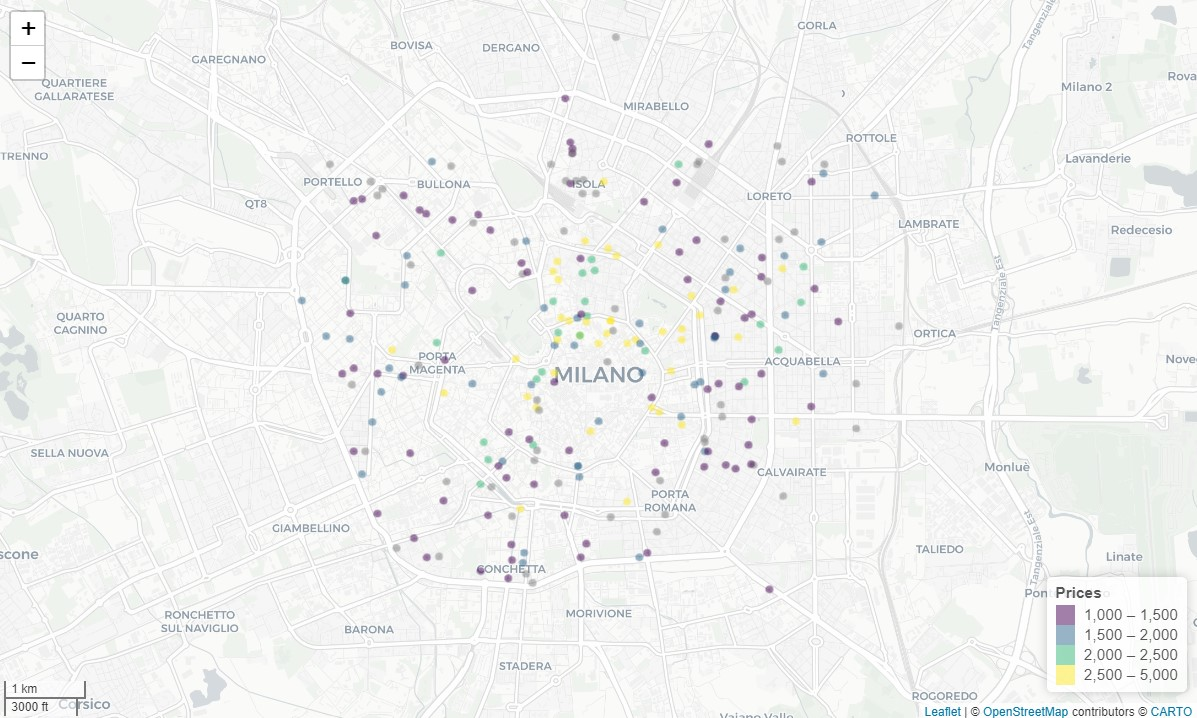
\includegraphics[width=1\linewidth]{images/leaflet_prezzi} \caption{Leaflet Map}\label{fig:LeafletVisuals}
\end{figure}

Predictors, in this case latitude and longitude appear to have nonlinear relationships with the outcome price. The relationship appears to be Gaussian whose mean points to the city center, red dashed line represent latitude and longitude coordinates for the Dome of Milan. Non linearities can be treated with regression splines

\begin{figure}
\centering
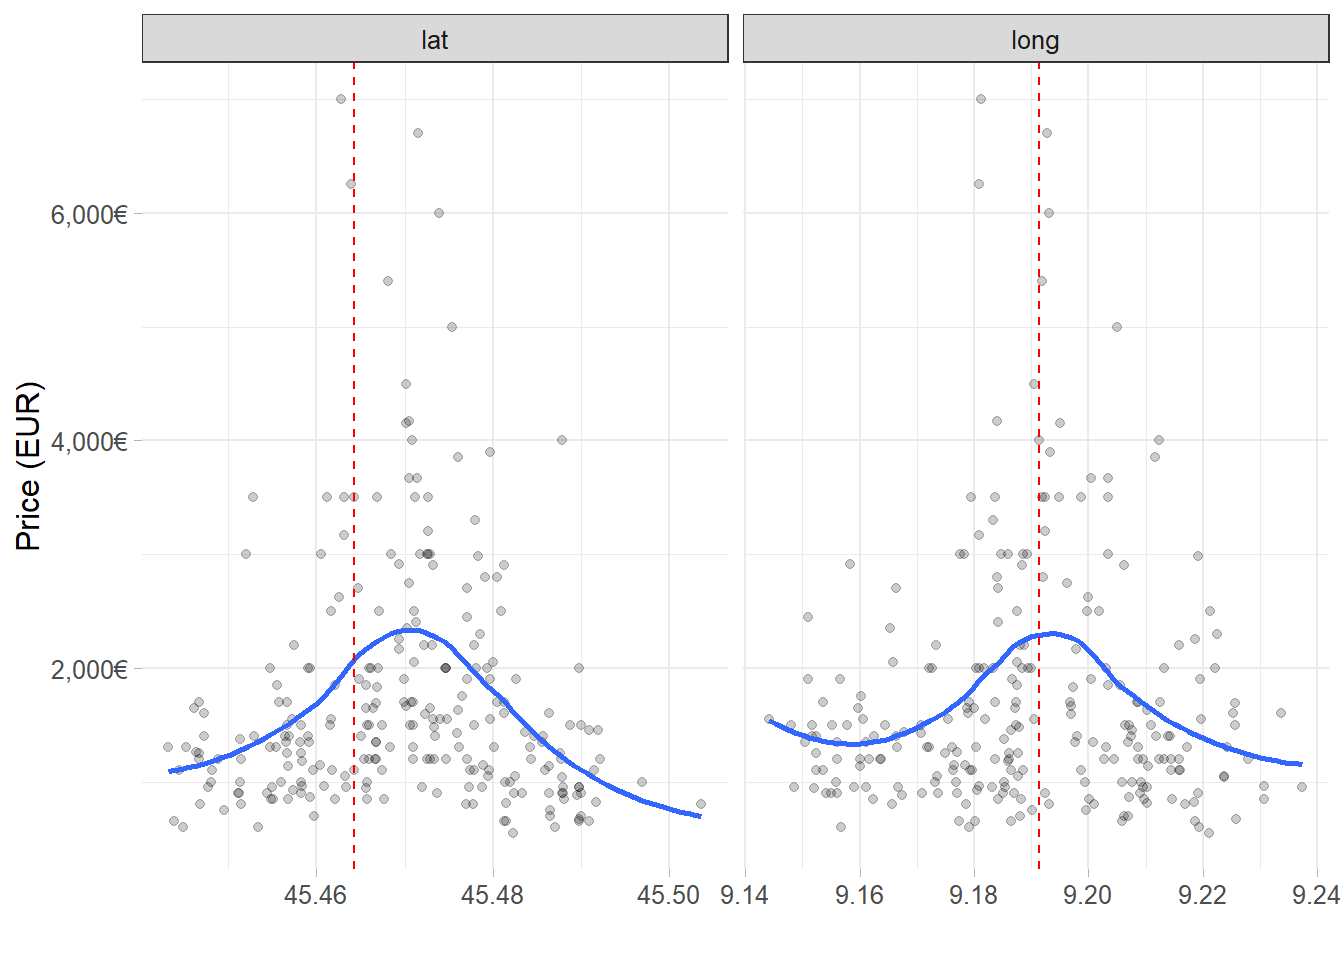
\includegraphics{07-exploratory_files/figure-latex/NonLinearSpatialRel-1.pdf}
\caption{\label{fig:NonLinearSpatialRel}Non Linear Spatial Relationship disclosed}
\end{figure}

ggplot2 visualzitaion matt dancho inspiration::

\hypertarget{counts-and-first-orientations}{%
\section{Counts and First Orientations}\label{counts-and-first-orientations}}

Arranged Counts for categorical columns can give a sense of the distribution of categories across the dataset suggesting also which predictor to include in the model. The visualization in figure \ref{fig:fctCounts} offers the rearranged factor \emph{TOTLOCALI}.
Bilocali are the most common option for rent, then trilocali comes after. The intuition behind suggests that Milan rental market is oriented to ``lighter'' accommodations in terms of space and squarefootage. This should comes natural since Milan is both a vivid study and working area, so short stayings are warmly welcomed.

\begin{figure}
\centering
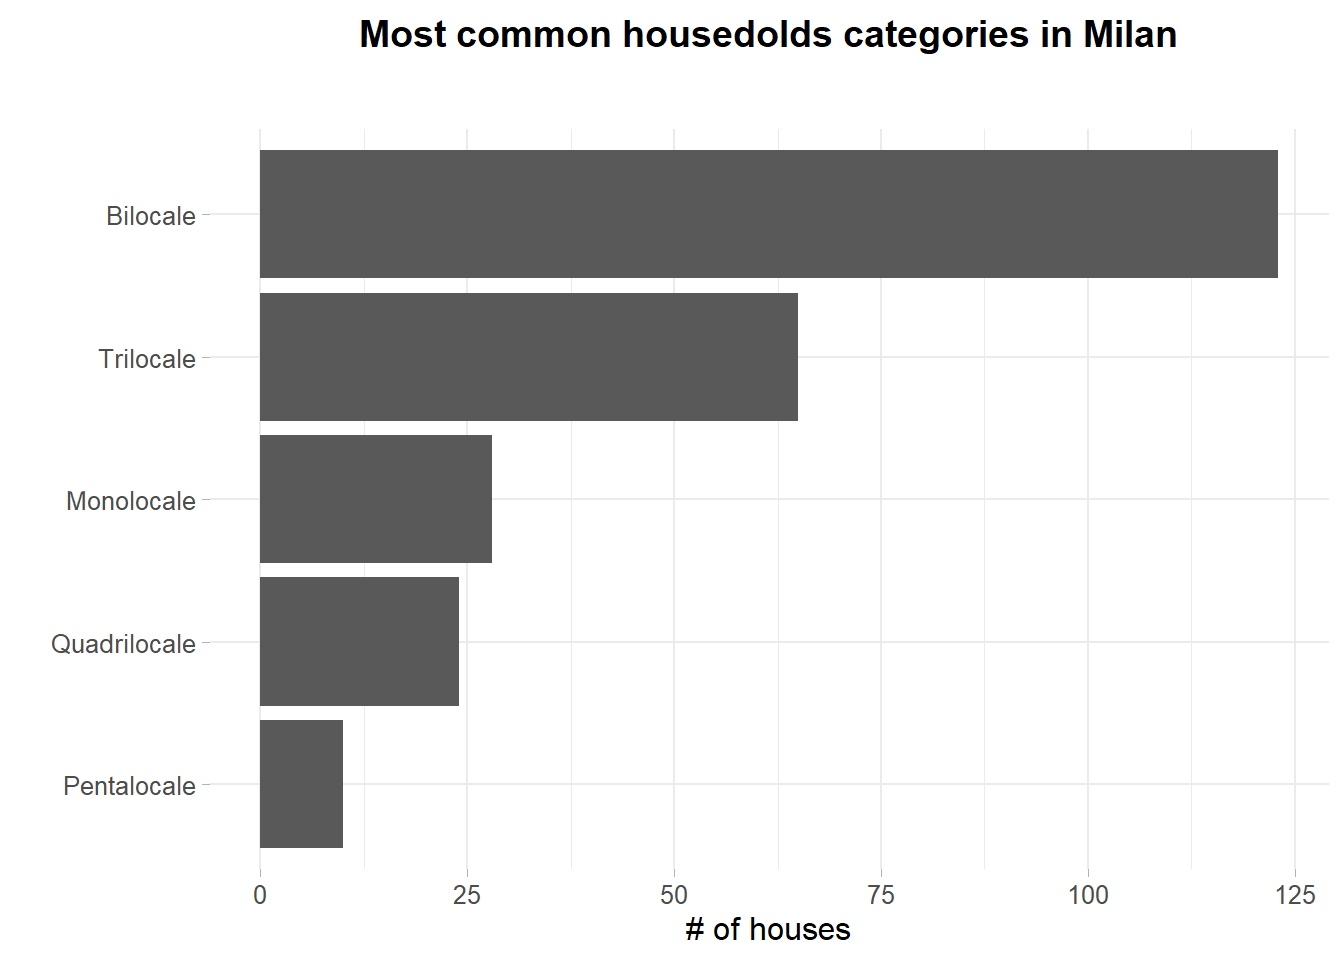
\includegraphics{07-exploratory_files/figure-latex/fctCounts-1.pdf}
\caption{\label{fig:fctCounts}Most common housedolds categories}
\end{figure}

Two of the most requested features for comfort and livability in rents are the heating/cooling systems installed. Moreover rental market demand, regardless of the rent duration, strives for a ready-to-accomodate offer to meet clients needs. In this sense accomodation coming with the newest and most techonological systems are naturally preferred with respect the contrary.
x-axis in figure \ref{fig:PricePerAc} represents log\_10 price for both of the two plots. Logarithmic scale is needed to smooth distributions and the resulting price interpretation have to considered into relative percent changes. Furthermore factors are reordered with respect to decreasing price.\\
y-axis are the different level for the categorical variables recoded from the original data due to simplify lables and to hold plot dimension. Moreover counts per level are expressed between brackets close to their respective factor.
The top plot displays the most prevalent heating systems categories, among which the most prevalent is ``Cen\_Rad\_Met'' by far. This fact is extremely important since metano is a green energy source and if the adoption is wide spread and pipelines are well organized than it brings enormous benefit to the city. As a consequence one major concern regards that for many years policies have been oriented to reduce vehicles emission (euro1 euro2\ldots) instead of focusing on house emissions. This was also a consequence of the lack of house data especially in rural areas. According to data there are still a 15\% portion of houses powered by oil fired.
Then in bottom plot Jittering is then applied to point out the number of outliers outside the IQR (Inter Quantile Range) .25 and their impact on the distribution. A first conclusion is that outliers are mainly located in autonomous systems, which leads of course to believe that the most expensive houses are heated by autonomoius heating systems. Indedd in any case this fact that does not affect monthly price. The overlapping IQR signifies that the covariates levels do not impact the response variable.

\begin{figure}
\centering
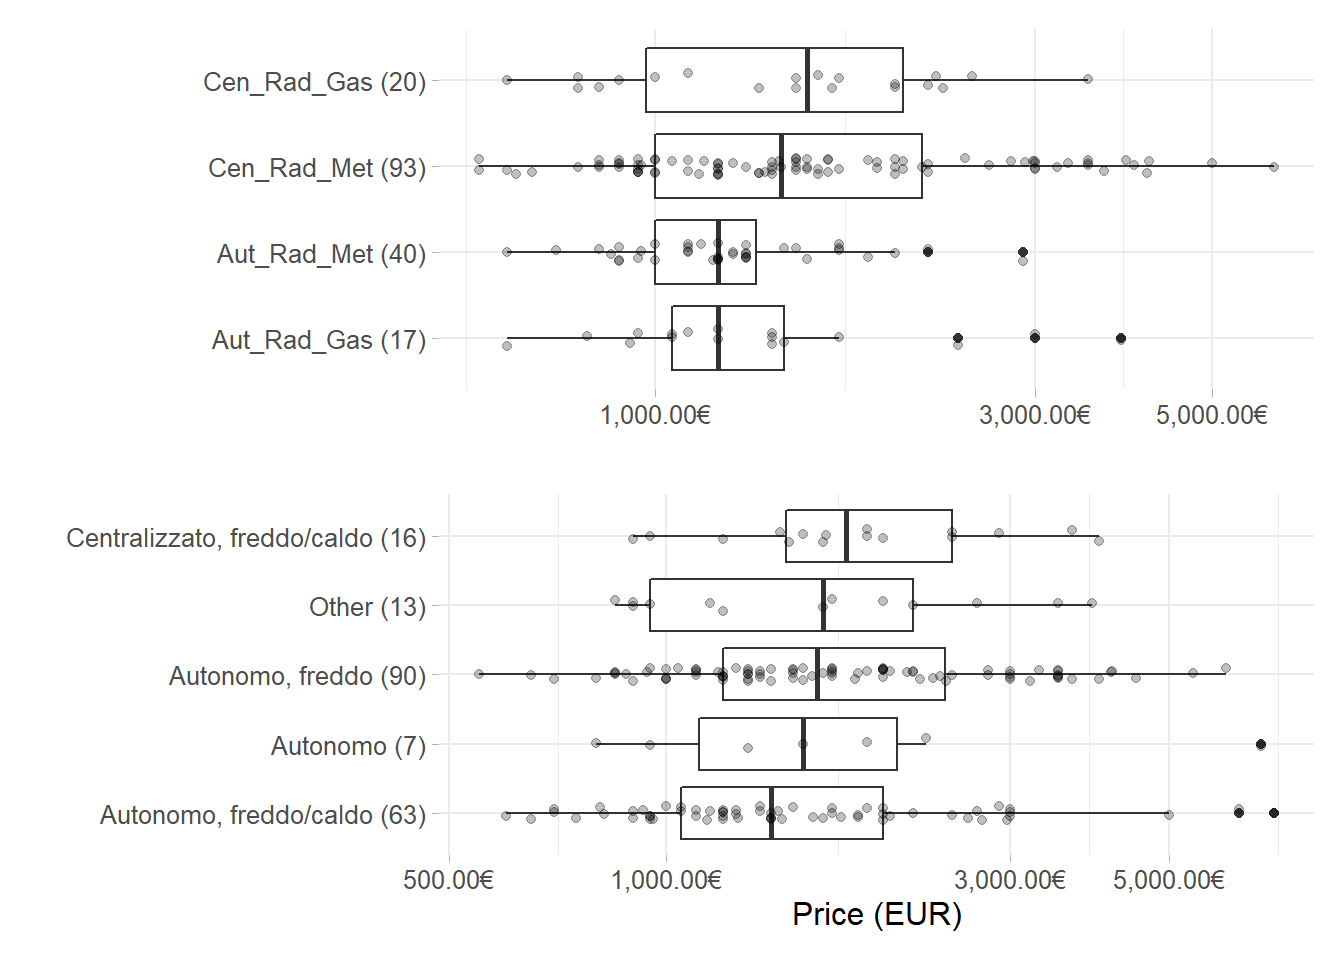
\includegraphics{07-exploratory_files/figure-latex/PricePerAc-1.pdf}
\caption{\label{fig:PricePerAc}Log Monthly Price per Heating/Cooling system?}
\end{figure}

this visualization intersects allows to discover bimodality in the response variable. Log scales was needed since they are all veru skewd and log scale then is needed also in the model.

(qui ci puoi mettere a confronto per variabile bianria, così vedi cosa includere nel modello esempio sotto dove commentato, )

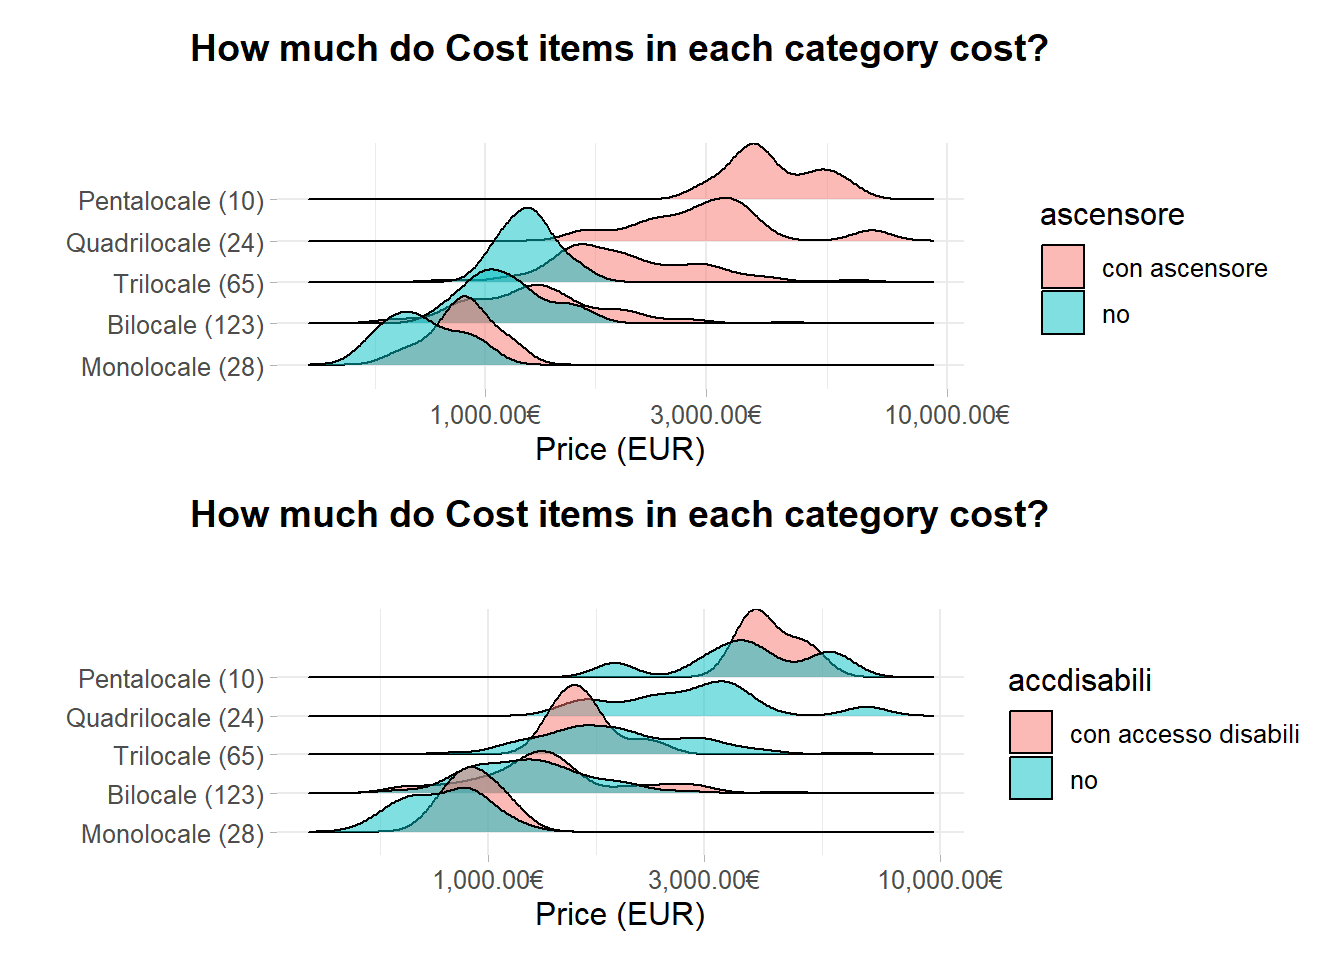
\includegraphics{07-exploratory_files/figure-latex/unnamed-chunk-1-1.pdf}

What it might be really relevant to research is how monthly prices change with respect to house square footage for each house configuration. The idea is to asses how much adding a further square meter affetcs the monthly price for each n-roomed flat.
One implication is how the property should be developed in order to request a greater amount of money per month. As an example in a situation in which the household has to lot its property into different sub units he can be helped to decide the most proficient choice in economic terms by setting ex ante the square footage extensions for each of the sub-properties.
A further implication can regard economic convenience to enlarge new property acquisitions under the expectation to broadened the square footage (construction firms). Some of the potential enlargements are economically justified, some of the other are not.
The plot \ref{fig:GlmPriceSq} has two continuous variables for x (price) and y (sqfeet) axis, the latter is log 10 scaled due to smoothness reasons. Coloration discretizes points for the each \(j\) household rooms totlocali. A sort of overlapping piece-wise linear regression (log-linear due to transformation) is fitted on each totlocali group, whose response variable is price and whose only predictor is the square footage surface (i.e.~\(\log_{10}(\mathbf{price_j}) \sim +\beta_{0,j}+\beta_{1,j}\mathbf{sqfeet_j}\)). Five different regression models are proposed in the top left. The interesting part regards the models slopes \(\hat\beta_{1,j}\). The highest corresponds to ``Monolocale'' for which the enlargement of a 10 square meters in surface enriches the apartment of a 0.1819524\% monthly price addition. Almost the same is witnessed in ``Bilocale'' for which a 10 square meters extension gains a 0.1194379\% value. One more major thing to notice is the ``ensamble'' regression line obtained as the interpolation of the 5 plotted ones. The line suggests a clear slope descending pattern (logarithmic trend) from Pentalocale and beyond whose assumption is strengthened by looking at the decreasing trend in the \(\hat\beta_1\) predictor slopes coefficients. Furthermore investing into an extension for ``Quadrilocale'' and ``Trilocale'' is \emph{coeteris paribus} an interchangeable economic choice.

\begin{figure}
\centering
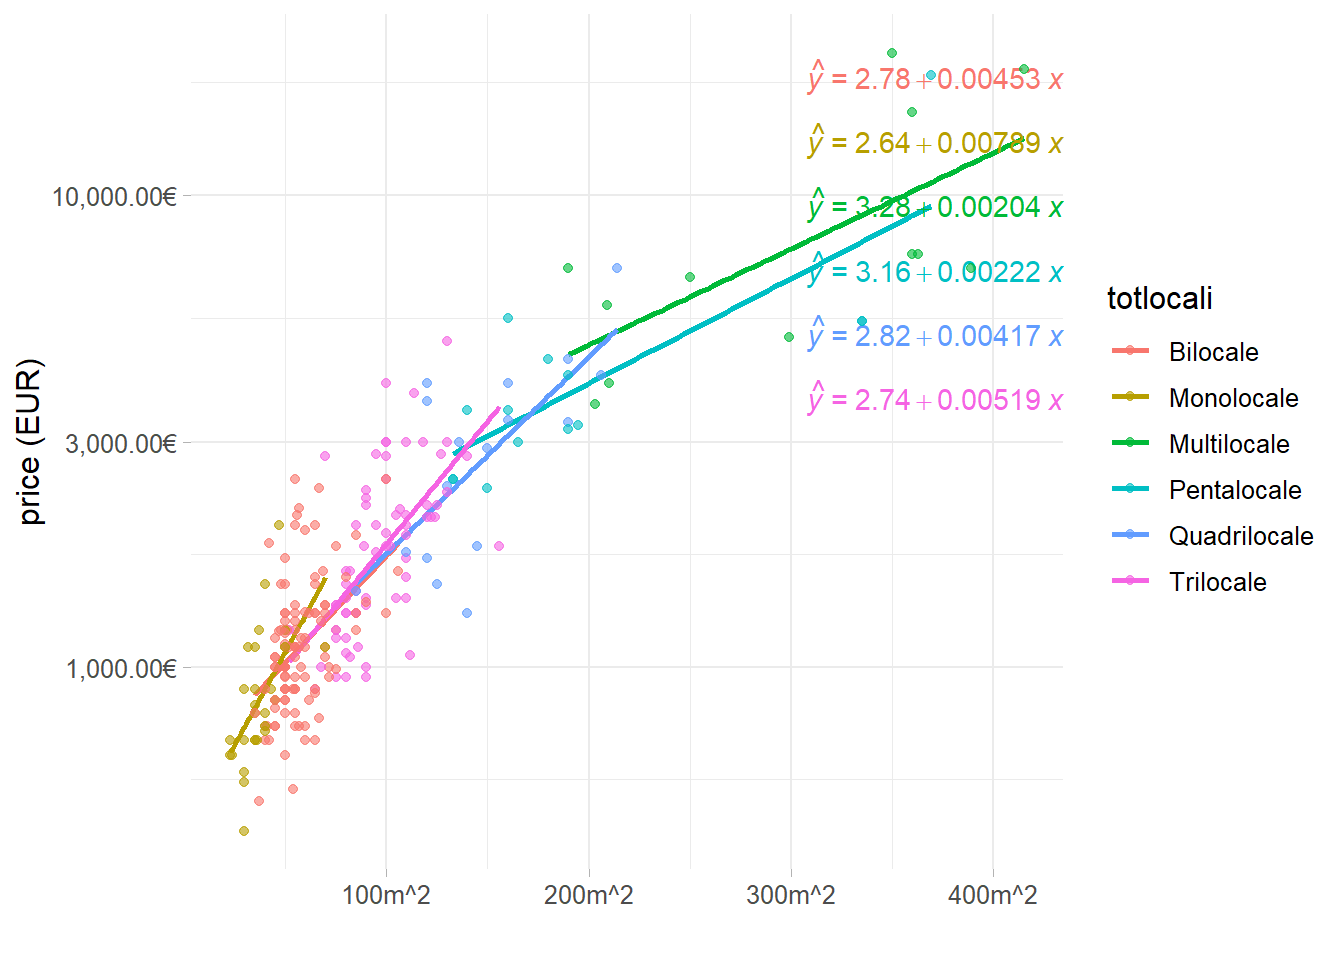
\includegraphics{07-exploratory_files/figure-latex/GlmPriceSq-1.pdf}
\caption{\label{fig:GlmPriceSq}Monthly Prices change wrt square meters footage in different n-roomed apt}
\end{figure}

In table (\ldots) resides the answer to the question ``which are the most profitable properties per month in terms of the price per square meter footage ratio''. The covariate floor together with the totpiani are not part of the model, indeed they can explain the importance and the height of the building justifying extraordinary prices. The first 4 observations are unsurprisingly ``Bilocale'', the spatial column location, not a regressor, can lend a hand to acknowledge that the street addresses point to very central and popular zones. The zones are, first City Life, second Brera and third Moscova, proving that in modeling real estate rents the spatial component is fundamental , even more in Milan.

\begin{tabular}{llrrllr}
\toprule
location & totlocali & price & sqfeet & floor & totpiani & abs\_price\\
\midrule
viale cassiodoro 28 & Bilocale & 1750 & 30 & 9 piano & 10 piani & 58.33333\\
via della spiga 23 & Bilocale & 2750 & 55 & 2 piano & 4 piani & 50.00000\\
corso giuseppe garibaldi 95 & Bilocale & 2700 & 56 & 2 piano & 5 piani & 48.21429\\
piazza san babila C.A. & Bilocale & 1833 & 42 & 4 piano & 4 piani & 43.64286\\
ottimo stato piano terra, C.A. & Trilocale & 3000 & 80 & Piano terra & 3 piani & 37.50000\\
\addlinespace
via federico confalonieri 5 & Monolocale & 750 & 20 & 1 piano & 3 piani & 37.50000\\
\bottomrule
\end{tabular}

Then as a further point it might be important to investigate a linear model whose response is price and whose covariates are the newly created abs\_price and some other presumably important ones e.g.~floor, bagno, totpiani. The model fitted is \passthrough{\lstinline!log2(price) \~ log2(abs\_price) + bagno + floor + totpiani!}.
The plot in figure \ref{fig:TieFighterPlot} has the purpose to demonstrate how monthly price is affected by covariates conditioned to their respective square meter footage. The interpretation of the plot starts by fixing a focus point on 0, which is the null effect highlighted by the red dashed line. Then the second focus is on house surface effect (i.e.~House Surface (doubling) in the plot, the term log2(abs\_price) has been converted to more familiar House Surface (doubling)), which contributes to increase the price of an estimated coefficient of \(\approx .6\) for each doubling of the square meter footage. Then what it can be noticed with respect to the two focus points are the unusual effects provoked by the other predictors t the right of the house surface effect and to the far left below 0. ``2 and 3 bagni'' are unusually expensive with respect to the square meter footage increment, on the other hand" al piano rialzato" and ``al piano terra'' are undervalued with respect to their surface. The fact that 2 and 3 bathrooms can guarantee a monthly extra check is probably caused to a minimum rent plateau requested for each occupant. the number of bathrooms are a proxy to both house extension since normally for each sleeping room there also exist at least 1 bathroom as well as prestigious houses dispose of more than 1 toilette services. So the more are the occupants regardless of the square meter footage dedicated to them, the more the house monthly returns,

it can be noticed is that ultimo piano, otgether with 2 abagni ad 3 bagni are unusually expensive with respect to their proper square meter footage. On the other hand the piano rialzato and piano terra are unusually undervalued given their surface.\\
In other words the to help with the interpretation. The fact that 2 and 3 bathrooms can guarantee a monthly extra check is probably caused to a minimum rent plateau requested for each occupant. So the more are the occupants regardless of the square meter footage dedicated to them, the more the house returns. The conclusion

\begin{figure}
\centering
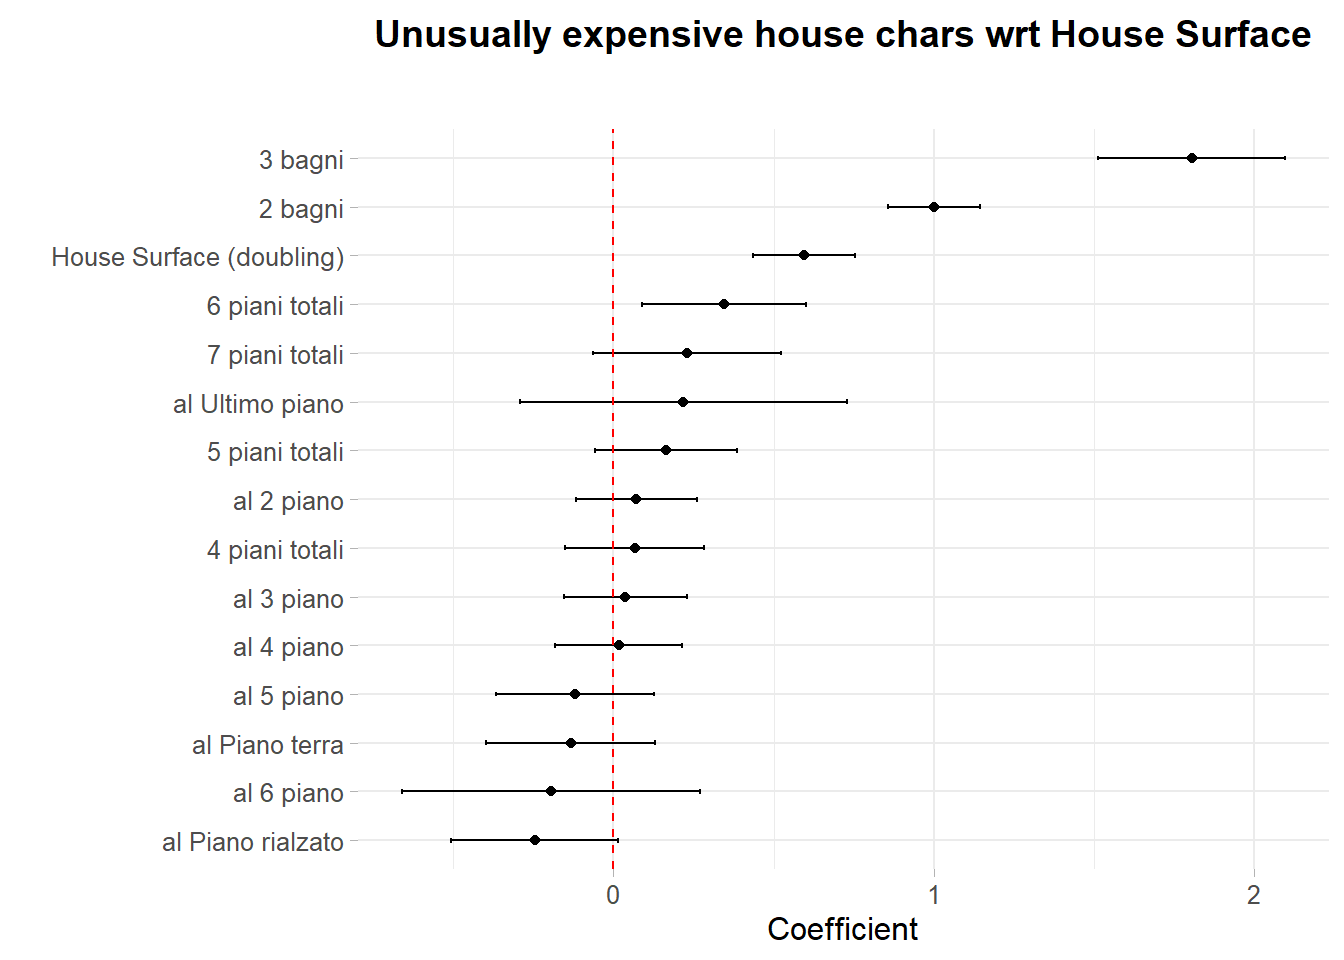
\includegraphics{07-exploratory_files/figure-latex/TieFighterPlot-1.pdf}
\caption{\label{fig:TieFighterPlot}Coefficient Tie fighter plot for the linear model: log2(price) \textasciitilde{} log2(abs\_price) + condom + other\_colors}
\end{figure}

\hypertarget{text-mining-in-estate-review}{%
\section{Text Mining in estate Review}\label{text-mining-in-estate-review}}

The word network in figure \ref(fig:WordNetworkgraph) tries to summarize relevant information from real estate agency review into each advertisement. avg\_totprice expresses the sum of the price per month plus the condominium in order to fully integrate inner property characteristics together with building exclusivity. Tokenized words are then filtered with ``stopwords-iso'' italian dictionary.
Nodes associated with hotter colours are also associated to more expensive in and out-house characteristics. The size of nodes keeps track of the number of reviews in which the specific word appears. A table of the most common words can help highlight both the real estate jargon as well as words that brings up house values.

\begin{tabular}{lrrr}
\toprule
word & count & reviews & avg\_totprice\\
\midrule
bagno & 249 & 192 & 1888.622\\
cucina & 247 & 190 & 2088.814\\
ingresso & 194 & 173 & 1964.062\\
soggiorno & 182 & 159 & 1872.500\\
camera & 200 & 158 & 1936.945\\
\addlinespace
piano & 197 & 157 & 1982.234\\
arredato & 184 & 152 & 1744.614\\
composto & 158 & 146 & 1758.911\\
riscaldamento & 171 & 144 & 1877.404\\
zona & 282 & 139 & 1930.213\\
\bottomrule
\end{tabular}

Furthermore it is possible to grossly divide the plot in figure \ref(fig:WordNetworkgraph) into 3 sub-groups of nodes, each of which addresses a specific part of the house comprehensive evaluation.
In the far right side of the plot are considered the external appliances like neighbor stores, subway stations and services and are associated to mean prices. The correspondent number of reviews are not justifying by any type of price increasing effect. Whereas slightly moving the view to the left, the area centered in portineria evidences a sub-groups of nodes associated to relatively higher avg-totprice. Some of them are servizio signorile palazzo. The previous set of nodes indicates services that are proper to the building can lead to some sort of extra payment. Then still moving
Possiamo immaginare di dividere il network in 3 raggruppamenti di nodi, ognuno dei quali parla di uni specifico tema. nella parte alta sinistra csi parla delle circostanze estenre dell'appartamente, i negozi i mezzi serizi la metri, i prezzi evidenzziati dal colore nei nodi sono neutri, indicando che non impattano il prezzo in maniera significativa. poco più sotto è possibile vedere un altro centroide verso il quale puntano una serie di edges peritenti che riguardano i servizi interni al building come la portinerua, l'ingresso, il palazzo. in questo caso i colori sono più caldi e i servizi sembrano essere pagati di più. successivamente sosptandoci veros il centro del'network si nota un nodo di gravità attorno alquale si trovamo molti outgoing edges, che riscaldamento. Attorno a riscaldamento che vista la grandezza ricorre spesso nelle recensioni, si sviluppano tutti i servizi non descritti da immobiliare all'interno della casa, insiema a tutte le caratteristiche cbe distinguono la casa revisionata dalle altre. i colori degradano spostandosi da sinistra verso destea, accanto a riscaldmaento si nota un cluster che associati a prezzi minoro come spese condominiali e arredato arredato. nel caso delle spese condominiali i cluster sono associati a prezzi minori perchè il prezzo del conominio spesso non è commisurato al prezzo nè al prestigio dell'appartamento. Speso infatti include costi variabili come utenze gas e luce, o acqua che vengono scontati con prezzi più bassi di affitto. la somma di condominio e prezzo offrirebbe un panorama più chiaro.

\begin{figure}
\centering
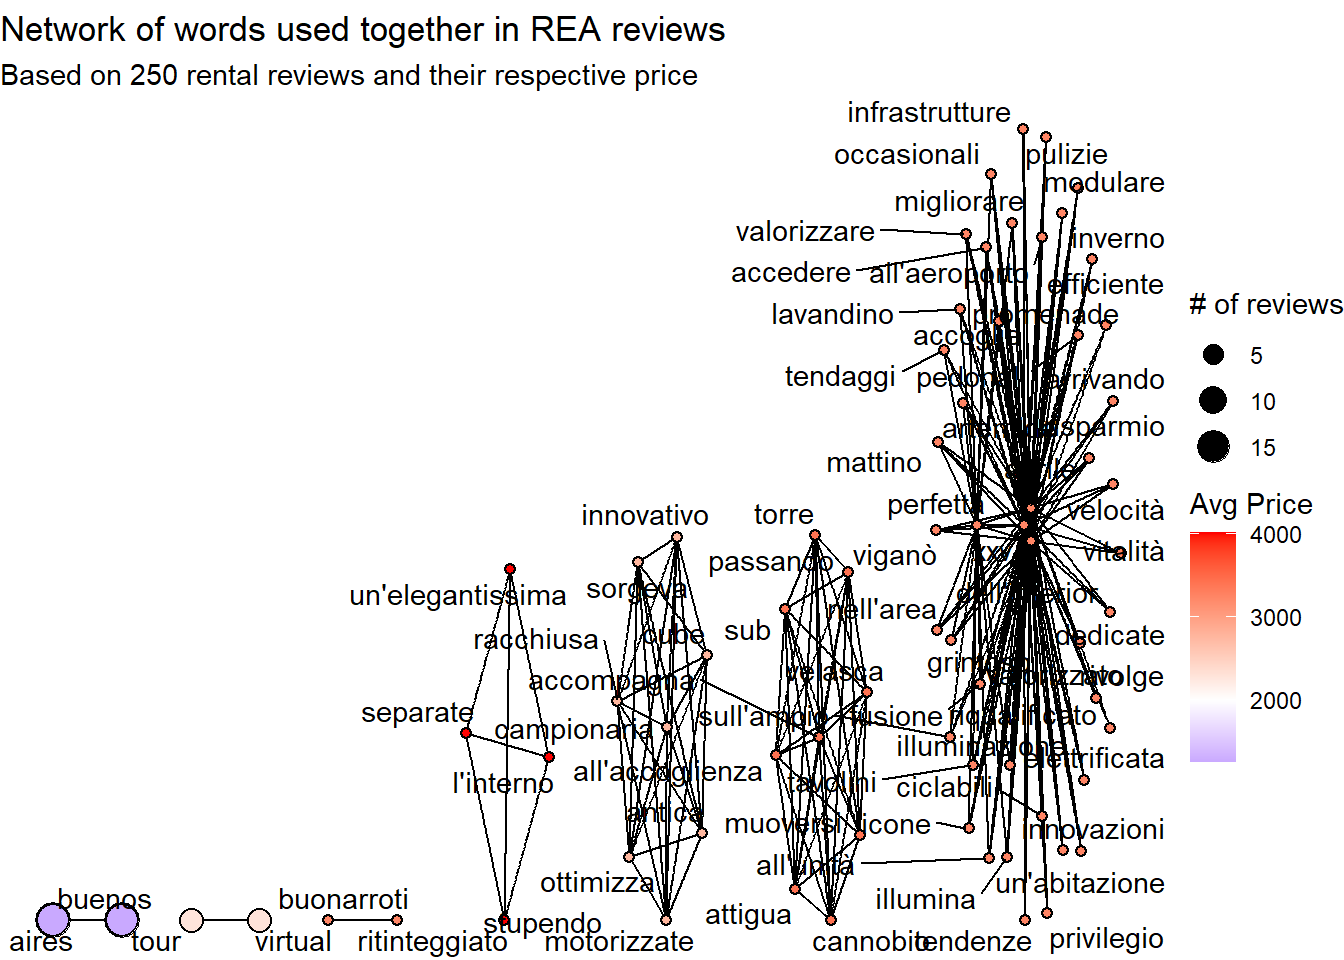
\includegraphics{07-exploratory_files/figure-latex/WordNetworkgraph-1.pdf}
\caption{\label{fig:WordNetworkgraph}Word Network Graph for 250 Estate Agencies Review}
\end{figure}

\hypertarget{missassimp}{%
\section{Missing Assessement and Imputation}\label{missassimp}}

As already pointed out some data might be lost since immobiliare provides the information that in turn are pre filled by estate agencies or privates through standard document formats. Some of the missing can be reverse engineered by other information in the web pages e.g.~given the street address it is possible to trace back the lat and long coordinates. Some other information can be encountered in .json files hidden inside each of the single web pages.
The approach followed in this part is to prune redundant data and rare predictors trying to limit the dimensionality of the dataset.

\hypertarget{missing-assessement}{%
\subsection{Missing assessement}\label{missing-assessement}}

The first problem to assess is why information are missing. As already pointed out in the preliminary part as well as in section \ref{ContentArchitecture} many of the presumably important covariates (i.e.~price lat, long, title ,id \ldots) undergo to a sequence of forced step inside scraping functions with the aim to avoid to be lost. If at the end of the sequence covariates are still missing, the correspondent observation is not considered and it is left out of the resulting scraped dataset. The choice originates from empirical missing patterns suggesting that when important information are missing then the rest of the covariates are more likely to be missing to, as a consequence the observation should be discarded.
The missing profile is crucial since it can also raise suspicion on the scraping failures. By Taking advantage of the missing pattern in observations the maintainer can directly identify the problem and derivatives and immediately debug the error. In order to identify if the nature of the pattern a revision of missing and randomness is introduced by \citet{Little}.
Missing can be devided into 3 categories:

\begin{itemize}
\tightlist
\item
  \emph{MCAR} (missing completely at random) likelihood of missing is equal for all the information, in other words missing data are one idependetn for the other.
\item
  \emph{MAR} (missing at random) likelihood of missing is not equal.
\item
  \emph{NMAR} (not missing at random) data that is missing due to a specific cause, scarping can be the cause.
\end{itemize}

MNAR is often the case of daily monitoring clinical studies \citep{Kuhn}, where patient might drop out the experiment because of death and so all the relating data starting from the death time +1 are lost.
To identify the pattern a \emph{heat map} plot \ref{fig:Heatmap} clarifies the idea:

\begin{figure}
\centering
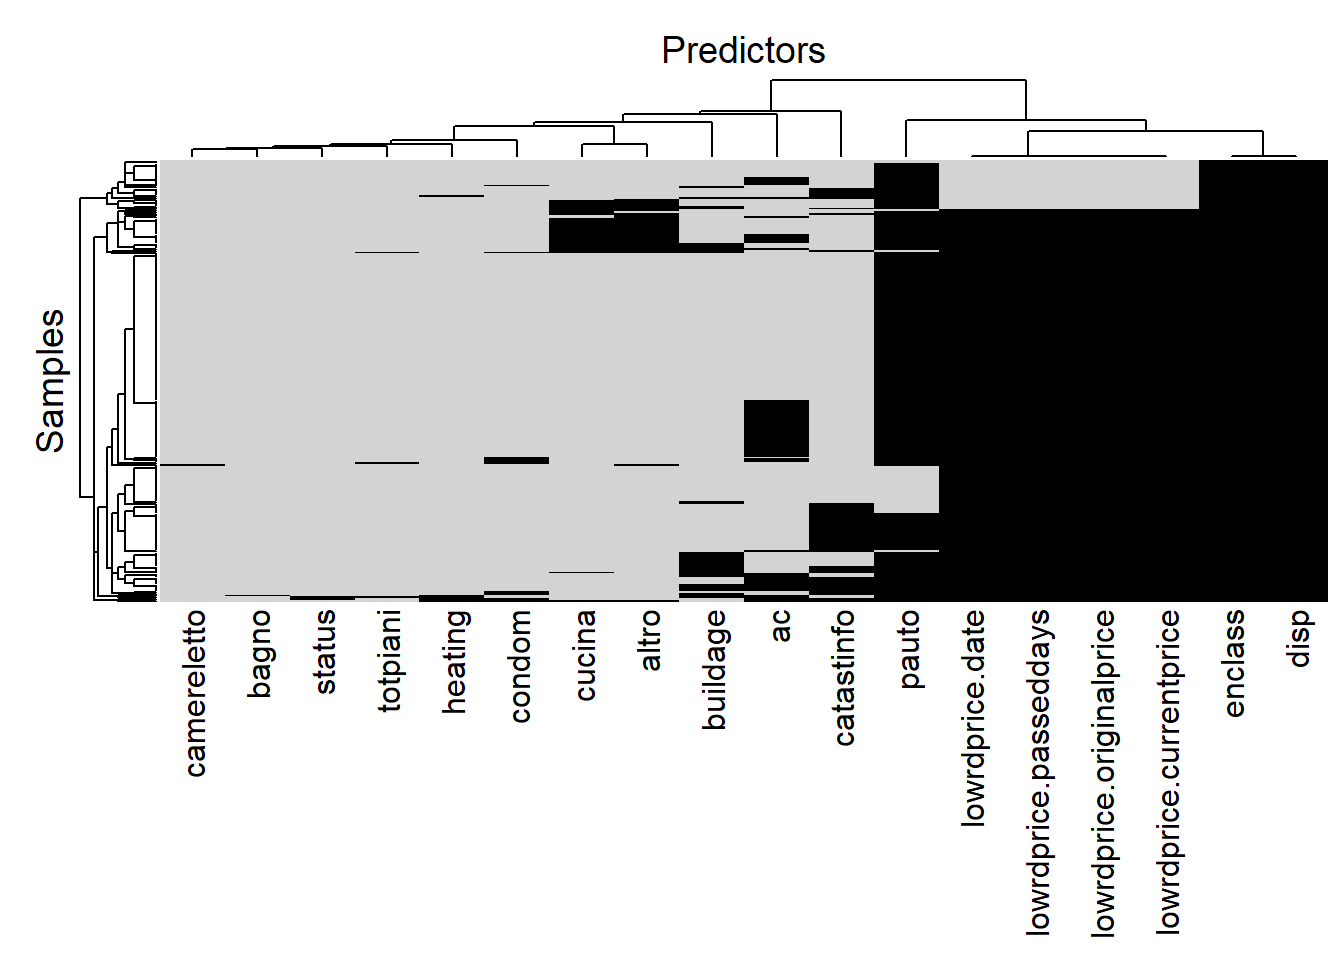
\includegraphics{07-exploratory_files/figure-latex/Heatmap-1.pdf}
\caption{\label{fig:Heatmap}Missingness Heatmap plot}
\end{figure}

Looking at the top of the heat map plot, right under the ``Predictor'' label, the first tree split divides predictors into two sub-groups. The left branch considers from \emph{TOTPIANI} to \emph{CATASTINFO} and there are no evident patterns. Then missingness can be traced back to MAR. Imputation needs to be applied up to \emph{CONDOM} included, the others are discarded due to rarity: i.e.~\emph{BUILDAGE}: 14\% missing, \emph{CATASTINFO}: 21\% and \emph{AC}: 24\%. Moreover \emph{CUCINA} and \emph{ALTRO} are generated as ``childred'' of the original \emph{LOCALI} variable, so it should not surprise that their missing behavior is similar ,whose prevalence is respectively 13\% and 14\%, for that reason are discarded.
In the far right hand side \emph{ENCLASS} and \emph{DISP} data are completely missing and a pattern seems to be found. The most obvious reason is a scraping fail in capturing data. Further inspection of the API scraping functions focused on the two covariates is strongly advised. From \emph{LOWRDPRICE.} covariates gorup class it seems to be witnessing a missing underlining pattern NMAR which is clearer by looking at the co\_occurrence plot in figure \ref{fig:cooccurrence}. Co-occurrence analysis might suggest frequency of missing predictor in combination and \emph{LOWRDPRICE.} class covariates are displaying this type of behavior. \emph{PAUTO} is missing in the place where \emph{LOWRDPRICE.} class covariates are missing, but this is not happening for the opposite, leading to the conclusion that \emph{PAUTO} should be treated as a rare covariate MAR, therefore \emph{PAUTO} is dropped.
After some further investigation on \emph{LOWRDPRICE.}, the group class flags when the \emph{PRICE} covariate is effectively decreased and this is unusual. That is solved by grouping the covariate's information and to encode it as a two levels categorical covariate if lowered or not. Further methods to feature engineer the \emph{LOWRDPRICE.} class covariates can be with techniques typical of profile data, further references are on \citet{Kuhn}.

\begin{figure}
\centering
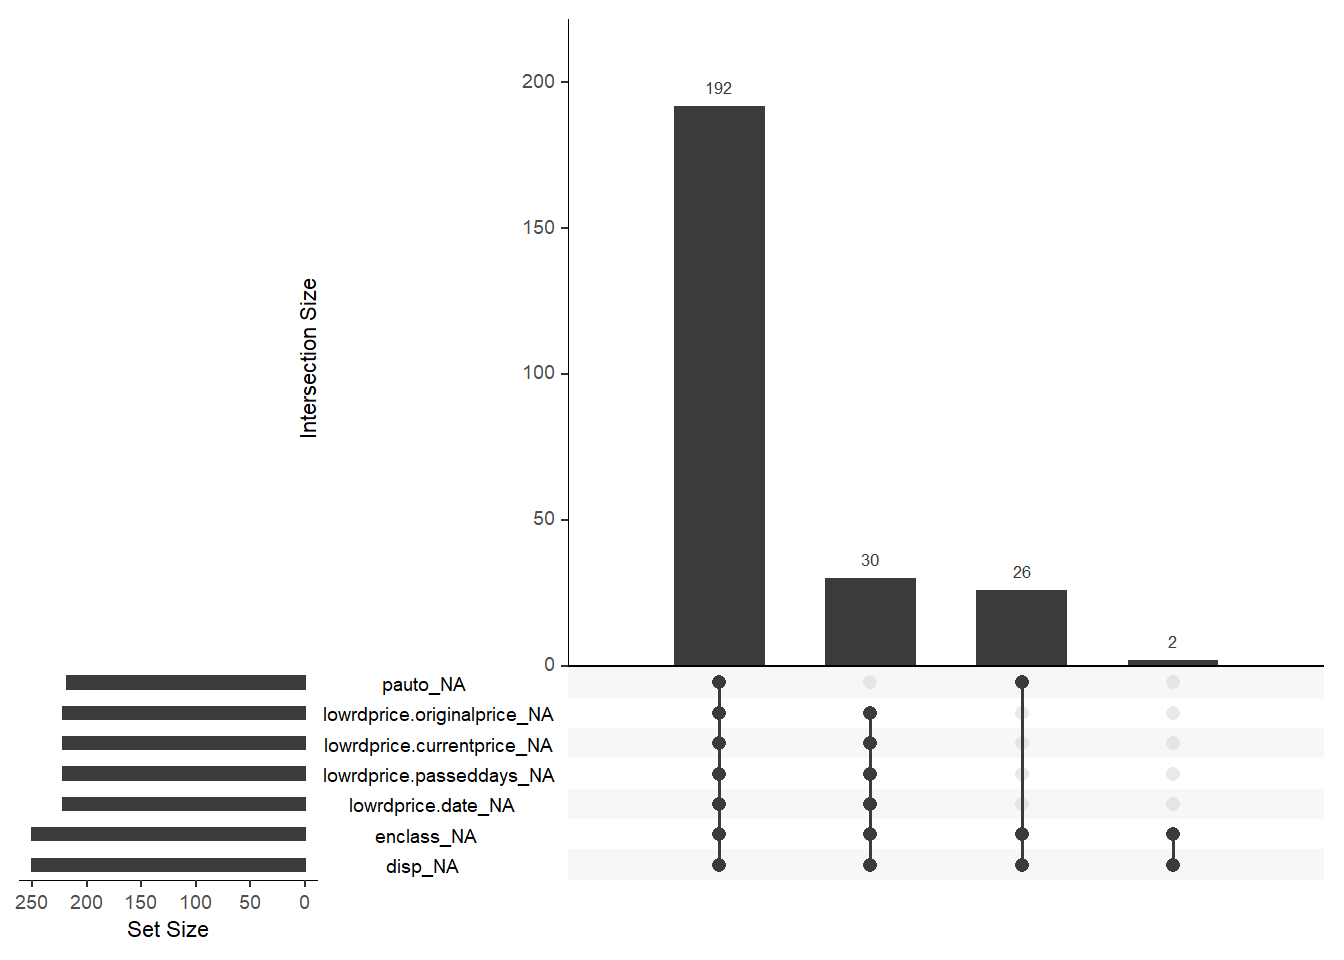
\includegraphics{07-exploratory_files/figure-latex/cooccurrence-1.pdf}
\caption{\label{fig:cooccurrence}Missingness co-occurrence plot}
\end{figure}

\hypertarget{covariates-imputation}{%
\subsection{Covariates Imputation}\label{covariates-imputation}}

A relatively simple approach to front missingness is to build a regression model to explain the covariates that have some missing and plug-back-in the respective estimates (e.g.~posterior means) from their predictive distributions \citet{Little}. This approach is fast and easy to implement in most of the cases, but it ignores the uncertainty behind the imputed values \citep{Bayesian_INLA_Rubio}. However it has the benefit to be a more than a reasonable choice with respect to the number of computation required, especially with INLA and in a spatial setting. That makes it the first choice method to follow since imputation regards also a small portion of data and predictors. At first it is considered the predictor \emph{condominium} for which some observation are missing. Indices are:

\begin{lstlisting}
##  [1]  19  74  77  90  99 113 116 120 179 249
\end{lstlisting}

A model is fitted based on missing data for which the response var is condominium and predictors are other important explanatory ones, i.e.\passthrough{\lstinline!condom \~ 1 + sqfeet + totlocali + floor + heating + ascensore!}. In addition to the formula in the inla function a further specification has to be provided with the command \passthrough{\lstinline!compute = TRUE!} in the argument control.predictor. The command \passthrough{\lstinline!compute!} estimates the posterior means of the predictive distribution in the response variable for the missing points. The estimated posetior mean quantities are then imputeda are in table @red(tab:CondomImputation)

\begin{tabular}{lrr}
\toprule
  & mean & sd\\
\midrule
fitted.Predictor.019 & 198.11095 & 19.67085\\
fitted.Predictor.074 & 162.96544 & 13.29456\\
fitted.Predictor.077 & 99.38197 & 32.34108\\
fitted.Predictor.090 & 331.73519 & 33.05035\\
fitted.Predictor.099 & 170.54068 & 12.30267\\
\addlinespace
fitted.Predictor.113 & 196.61593 & 15.86545\\
fitted.Predictor.116 & 108.40482 & 20.79689\\
fitted.Predictor.120 & 162.86977 & 25.61622\\
fitted.Predictor.179 & 165.03632 & 20.53485\\
fitted.Predictor.249 & 117.24234 & 30.80290\\
\bottomrule
\end{tabular}

A further method for imputation has been designed by \emph{Gómez-Rubio, Cameletti, and Blangiardo 2019) miss lit} by adding a sub-model for the imputations to the final model through the inla function. This is directly handled inside the predictor formula adding a parameter in the latent field. However the approach makes the model more complex with a further layer of uncertainty to handle.
At first the additive regression model with all the covariates is called including the covariates with missing values. The response variable \emph{PRICE} displays no missing values and the model fitted is:

\hypertarget{model-specification}{%
\section{Model Specification}\label{model-specification}}

\hypertarget{mesh-building}{%
\section{Mesh building}\label{mesh-building}}

\emph{PARAFRASARE}
The SPDE approach approximates the continuous Gaussian field \(w_{i}\) as a discrete Gaussian Markov random field by means of a finite basis function defined on a triangulated mesh of the region of study. The spatial surface can be interpolated performing this approximation with the inla.mesh.2d() function of the R-INLA package. This function creates a Constrained Refined Delaunay Triangulation (CRDT) over the study region, that will be simply referred to as the mesh. Mesh should be intended as a trade off between the accuracy of the GMRF surface representation and the computational cost, in other words the more are the vertices, the finer is the GF approximation, leading to a computational funnel.

\begin{figure}
\centering
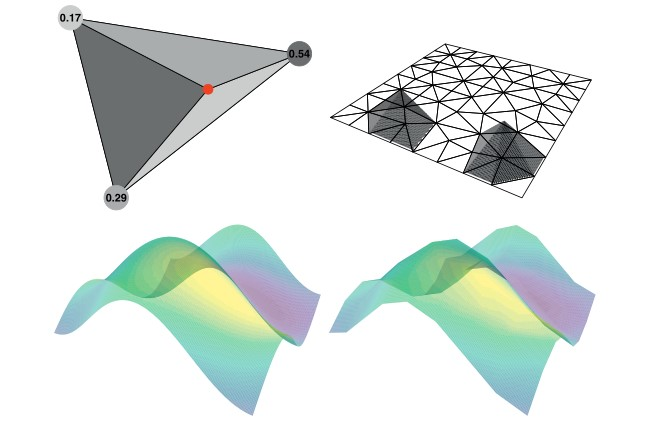
\includegraphics{images/triangle.jpg}
\caption{Traingularization intuition, \citet{Krainski-Rubio} source}
\end{figure}

Arguments can tune triangularization through inla.mesh.2d() :

\begin{itemize}
\tightlist
\item
  \passthrough{\lstinline!loc!}:location coordinates that are used as initial mesh vertices
\item
  \passthrough{\lstinline!boundary!}:object describing the boundary of the domain,
\item
  \passthrough{\lstinline!offset!}: argument is a numeric value (or a length two vector) and it is used
  to set the automatic extension distance. If positive, it is the extension distance
  in the same scale units. If negative, it is interpreted as a factor relative to the
  approximate data diameter; i.e., a value of -0.10 (the default) will add a 10\%
  of the data diameter as outer extension.
\item
  \passthrough{\lstinline!cutoff!}: points at a closer distance than the supplied value are replaced by a single vertex. Hence, it avoids small triangles
\item
  \passthrough{\lstinline!max.edge!}: A good mesh needs to have triangles as regular as possible in size and shape.
\item
  \passthrough{\lstinline!min.angle!}argument (which can be scalar or length two vector) can be used to specify the minimum internal angles of the triangles in the inner domain and the outer extension
\end{itemize}

A convex hull is a polygon of triangles out of the domain area, in other words the extension made to avoid the boundary effect. All meshes in Figure 2.12 have been made to have a convex hull boundary. If borders are available are generally preferred, so non convex hull meshes are avoided.

\hypertarget{shinyapp-for-mesh-assessment}{%
\subsection{Shinyapp for mesh assessment}\label{shinyapp-for-mesh-assessment}}

INLA includes a Shiny (Chang et al., 2018) application that can be used to tune the mesh params interactively

The mesh builder has a number of options to define the mesh on the left side. These include options to be passed to functions inla.nonconvex.hull() and inla.mesh.2d() and the resulting mesh displayed on the right part.

\hypertarget{building-spde-model-on-mesh}{%
\subsection{BUilding SPDE model on mesh}\label{building-spde-model-on-mesh}}

\hypertarget{fit.vgm-fit.variogramsemivar-vgmsph}{%
\chapter{fit.vgm = fit.variogram(semivar, vgm(``Sph''))}\label{fit.vgm-fit.variogramsemivar-vgmsph}}

\hypertarget{krg-krigelogprice-1-data-model-fit.vgm}{%
\chapter{krg = krige(log(PRICE) \textasciitilde{} 1, data, model = fit.vgm)}\label{krg-krigelogprice-1-data-model-fit.vgm}}

```

\hypertarget{modelspec}{%
\chapter{Model Selection \& Fitting}\label{modelspec}}

\hypertarget{model-criticism}{%
\section{Model Criticism}\label{model-criticism}}

evaluation of the variables to include in the mode,, assumptions of the model i.e.~exchangeablity and independence prior distribution to assign to parameters and hyper parameters.

\hypertarget{spatial-kriging}{%
\section{Spatial Kriging}\label{spatial-kriging}}

\hypertarget{model-checking-1}{%
\section{Model Checking}\label{model-checking-1}}

if (models \textgreater{} 2)\{

\begin{lstlisting}
## Model Selection




  IDEA: proporre due modelli uno più interepretabile con distribuzione normale, e un ò'altro con sempre exponential family ma con Gamma distribution function, ora vedo se riesco a fare tutto. dovrei sacrificare applicazione.
\end{lstlisting}

\}

\hypertarget{application}{%
\chapter{Shiny Application}\label{application}}

with UI build with free tool for front end design ion shiny \href{https://fomantic-ui.com/}{fomantic-ui}. prendi shiny app e rifai interface. in questo blog vedi Hacaton tirato e vincitori \href{https://blog.rstudio.com/2020/11/10/the-appsilon-shiny-semantic-pocontest/}{blog}.

Senno app paula moraga che ha già simil modello dentro,

senno flexdashboard paula moraga.

\href{https://demo.appsilon.ai/apps/polluter/}{this inspiration}

\hypertarget{appendix}{%
\chapter*{Appendix}\label{appendix}}
\addcontentsline{toc}{chapter}{Appendix}

\hypertarget{gpbasics}{%
\section{Gaussian Process}\label{gpbasics}}

Let assume ti have cloud of points represented by two variables \(X_1\) and \(X_2\), figure \ref{fig:gpcloud}. The cloud of points are observation taken from a realization of two variables e.g.~height and weight, What it might be observed is:

\begin{figure}
\centering
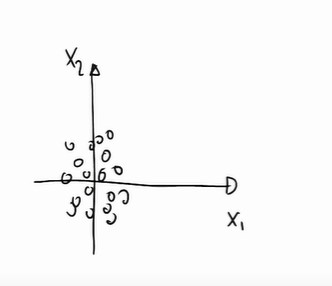
\includegraphics{appendix_images/gp_base_1.jpg}
\caption{\label{fig:gpclouds}Left panel: GP cloud of points fitted with a \emph{circle}, Right panel: GP cloud of points fitted with a \emph{ellipse}, source \citet{YT:freitas1}}
\end{figure}

Each circle in both panels figure \ref{fig:gpclouds} represents a measurements of the observed phenomenon. Let assume to fit a multivariate gaussian distribution to the left panel data. The process of learning is to fit a Gaussian to data, the ultimate goal is to describe the data, the most perfectly evident Gaussian is the one interpolating the points and centering in \(\left(0,0\right)\), a circle might be a good guess. Instead for the right one in \ref{fig:gpclouds}, a smart guess could be still centering the mean in, indeed now it is an ellipse describing the variability.
At this point it might be interesting to vectorized what is has been measured, the centers are then compressed into a vector \(\mu_{i}\), i.e.~it has two components \(X_1\) and \(X_2\) whose corresponding mean is 0.

\[
\boldsymbol{\mu}=\left[\begin{array}{ll}
\mu_{x_1} \\
\mu_{x_2}
\end{array}\right]
\]

This is true for all the observations which have two coordinates too \(x_1\) and \(x_2\). for each of the points, e.g.~for point 1:

\[
\mathbf{x_1}=\left[\begin{array}{ll}
x_1 \\
x_2
\end{array}\right]
\]

the can be neagtive positive, the Real numbers, usually we have \(\mathbb{R}^{2}\) extending from - infinity to + infinity, to the power of two because we have 2 dimensions, a Real plane.
any point is gaussian distributed when with mean .. an variance.
how we explain covariance, thorugh \emph{correlation.}
we do it by correlation with its noraml forms. the covariance is the term that goes insisde the matrices in the upper right of the matrxi we have the expectation of \(x_1\) times \(x_2\), like \(\mathbb{E}(x_1 \cdot x_2)\), where the extactation in the gaussian case is the mean which is 0, so the corresponding values is 0.
the covariance essentially is the dot product \href{https://mathinsight.org/dot_product_matrix_notation}{ref dot product} of \(x_1\) and \(x_2\) variable, so what happens when you take the dot product of vectors,
if for example you take a vector that looks like 1 and 0 and you take the dot product of one other vecto 1 and 0, so that:

\[
\left[\begin{array}{ll}
1 \\
0
\end{array}\right]\left[\begin{array}{ll}
1 & 0 \\
\end{array}\right] = 1
\]
You will end up with 1, recall dot productm first element first vcetor times first element second vectro and second element first vector times second element secon vector. So identical vector will get a high dot product value leading to a high similarity measure. Dot product can be indeded as a similarity measure.
\ldots{} But if you take two different vector as 1 0 and 0 1 then:

\[
\left[\begin{array}{ll}
1 \\
0
\end{array}\right]\left[\begin{array}{ll}
0 & 1 \\
\end{array}\right] = 0
\]

This time the multiplication leads to 0 value, as a matter of fact they are different. They are no similar.
IF two points are closed the dot product will be high in 2D. What the covariance should be? if variances are assumed to be 1 then in this case i qould expect to be 0, i.e.~covariance matrix is:

\[
\left[\begin{array}{ll}
1 & 0 \\
0 & 1
\end{array}\right] = \mathbf{cov_{plot1}}(x_1,x_2)
\]

because I can picka poin tin two pointa in this cloud. Suppose i increase x1 then my chance of getting a x2 point that is positive or negative is the samee, knowing somthin about x1 give nothign about x2. no information is proivede. On the other hand i the second plot knowing a positive value of 1 can suggest with a certain probability that x2 will be positive (great proabibility. So some information is provided), e.g.

\[
\left[\begin{array}{ll}
1   & 0.5 \\
0.5 & 1
\end{array}\right] = \mathbf{cov_{plot2}}(x_1,x_2)
\]

Some positive number idicates that i expect a positive inc rease iwhen boht of the two are increasing singularly. thsi is what the correlation, the basis to do linear regresssion and non linear- thei is a bivariate gaussian. If the entri3es are means that they are uncoorellated, if they are non-zero then they are correlated, theby can be both positive or negative (correlatiob)

now lets generate a gassiian distrivution so x\_1 and x\_2 in 2D and then a third dimension hwere we express probability, this is said joint distribution. So i am going to cu this gaussian at certain point for x\_1 and cut a plain rigght thgouth this gauissan imagine to ahava cake and then taka kkniw and cut it.(see the image)

form the man perspective you are goin to see a gaussian distribution, you will be lookong at x\_ and you will be seeing a gaussain plot in green. this is the probability of x\_1 gievn x\_1. also said ``conditioned'' probabolity. This gaussian has a mean like the one alreasdy seen and this is the center of the gaussian, we can rewrite the mena and variance of the multivariate gaussian describing the cloud of points. sigma are the covaraince martix sigma.

\ldots{}
sigma 1 and signa 2 if you have 1 d varibale the widjth has to be postive, for mulitvariate gaussian equl so here positive definitness: covariance mateix symetric.\\
\ldots{}
any artibitray variable transposed x time the covarince matrix nedds to be positive.
what is the mean of this gaussian i might want to know what is the widht of this gaussian would it be great if there is a formula that guven the cloud of point and likelihood estimation. we coilf obtain the red bell in figure.
Compute the green curve how it is done? this requires some work and it is said matrix \emph{invesrion lemma}, this is foudamental for machine learnign. let's assume it. The theorem says that the the mean fof the gaussian is the mean of x\_1 and then some other operation with sigma, see below from paci (miss ref)

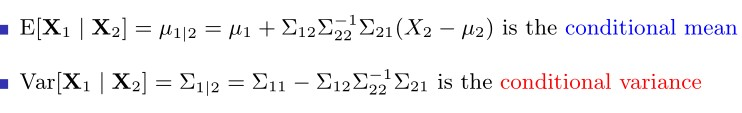
\includegraphics{appendix_images/inverse_lemma.jpg}
the theorem says toi ocnsider a multivariate gaussian a vector 1 and a vector 2 each vecto compinent has a mena and a covarianc matrix, this by lemma gives us the expression and the math behind is no tremendous, but it is long. What it is important is to undestand fto go from a joont to a conditional distribution in our case. thats i the value od the theorem.

One background further thing: assume that we have a gaussian variable distribution that we want to sample fromm, we had now ewe are going to do the opposite, before we had poitns and we tried to figure out the curve, now we have the curve and we are gointg to try to rpoduce data. I need to be able to draw sample froma gaussian distribution. i will assume that i have a meachnism that produces a uniform samples, so you have a random numebr generatior with equal probabolity from 0 to 1, I assume a also the cumulative aof a gaussian.

the cumulative of a gaussian is what you get if you syrta summing the area under the curve of the gaussian as you move from the left. value after valure you can plot the cumulative ahead (see figure) the point where there is a flex point is the mean beacuse tha gassias is symmetric. The asymptot is 1 becuase the are under the curve sumes to 1.
If i can draw a random number form Uniform and the project it to thre cumulative and then finally projct it back to the gaussian distribution. Inverse cumulative mapping. If oyu do this multiple times you are going to have many sample palced next to the mean and as sparse as the variance. in this process of sampling try to sample a point i froma gaussian that has mean 0 a variance 1, now letes try to draw a point from a gaussian with mean mu and variance sigma. \ldots{}

In the multivariate case suppose that we have evctor with two variables how do i draw a vector from a multivariate gasussian with 0 means and plot 1 covarianc ematrix. the theormeem also says that the marginal distribution can be seen by civariance matrix , fist take the men\_1 and take upper left element from the covariance matrix obtaining the marginal rpobabiloty for x\_1, i.e.

Then for simplicity we can simplyfy by groupign vector into:
(vectore exoression multivariate)

I need a wau to take square trotto of matrices, if x come sfroma MVG

35:01--

\hypertarget{triangular}{%
\section{\texorpdfstring{SPDE and Triangularization (YT speech: \citet{YT:paumoraga})}{SPDE and Triangularization (YT speech: @YT:paumoraga)}}\label{triangular}}

In order to fit LGM type of models with a spatial component INLA uses SPDE (Stochastic Partial Differential Equations) approach.
Suppose that is it given have a continuous Gaussian random process (a general continuous surface), what SPDE does is to approximate the continuous process by a discrete Gaussian process using a triangulation of the region of the study. Let assume to have a set of points defined by a CRS system (Latitude and Longitude, Easthings and Northings), and let assume that the object of the analysis is to estimate a spatially continuous process. Instead of exploiting this property as a whole, it is estimated the process only at the vertices of this triangulation. This requires to put a triangularization of the region of the study on top the the process and the software will predict the value of the process at its vertices, then it interpolates the rest of the points obtaining a ``scattered'' surface.

\begin{figure}
\centering
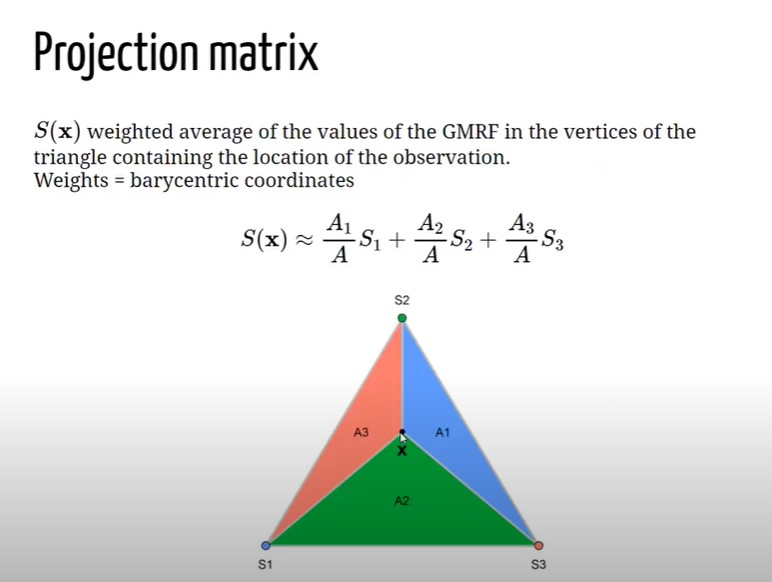
\includegraphics{appendix_images/appendix_triangularization.jpg}
\caption{\label{fig:triang}Triangulariation weights and associated process value, \citet{YT:paumoraga} source}
\end{figure}

Imagine to have a point a location X laying inside a triangle whose vertices are \(S_1, S_2 and S_3\). SPDE operates by setting the values of the process at location x equal to the value of the process at their vertices with some weights, and the weights are given by the \emph{Baricentric coordinates (BC)}. BC are proportional to the area at the point and the vertices. Let assume to have a piece of triangularization \(\boldsymbol{A}\) and let assume that the goal is to compute the value at location X. X, as in formula above \(\boldsymbol{A}\), would be equal to \(S_1\), multiplied by the area \(A_1\) dived by the whole triangle area (\(\boldsymbol{A}\)) + \(S_2\) multiplied by the area \(A_2\) divided by \(\boldsymbol{A}\) + \(S_3\), multiplied by the area \(A_3\) dived by (\(\boldsymbol{A}\). This would be the value of the process at location X given the triangulations (numeber of vertices). SPDE is actually apprximatring the value of hte process using a weighted average of the value of the process at the triangle vertices which ir proportional to the area of the below triangle.
In order to do this within INLA \ref{inla} it is needed also a \emph{Projection Matrix} , figure \ref{fig:projmat}. The Projection matrix maps the continuous GRMF (when it is assumed a GP) from the observation to the triangulation. It essentially assigns the hieght of the triangle for each vertex of the triangularization to the process. Matrix \(\mathcal{A}\), whose dimensions are \(\mathcal{A_{ng}}\). It has \(n\) rows a \(g\) columns, where \(n\) is the number of observations and \(g\) is the number of vertices of the triangulation. Each row has possibly three non-0 values, right matrix in figure \ref{fig:projmat}, and the columns represent the vertices of the triangles that contains the point. Assume to have an observation that coincides with a vertex \(S_1\) of the triangle in \ref{fig:triang}, since the point is on top of the vertex (not inside), there are no weights (\(A_1 = \mathcal{A}\)) and 1 would be the value at \(A_{(1,1)}\) and 0 would be the rest f the values in the row. Now let assume to have an observation coinciding with \(S_3\) (vertex in position 3), then the result for \(A_{(2,3)}\) would be 1 and the rest 0. Indeed when tha value is X that lies within one of the triangles all the elements of the rows will be 0, but three elements in the row corresponding of the p osition of the vertices \(1 = .2, 2 = .2 and g = .6\), as a result X will be weighted down for the areas.

\begin{figure}
\centering
\includegraphics{appendix_images/appendix_proj.jpg}
\caption{\label{fig:projmat}Projection Matrix to map valjes from tringulation back to the GP, \citet{YT:paumoraga} surce}
\end{figure}

  \bibliography{refs.bib,Rpackages.bib}

\end{document}
